\documentclass[a4paper, 14pt, oneside]{book}
\usepackage[utf8]{inputenc}
\usepackage[margin=1in]{geometry}

\title{Calculus}
\author{Rushil Surti}
\date{\today}

\usepackage{titlesec}

\usepackage[hidelinks]{hyperref}
\usepackage{microtype}
\usepackage{amsmath}
\usepackage{amssymb}
\usepackage{amsthm}
\usepackage{cancel}
\usepackage[usenames,dvipsnames]{xcolor}
\usepackage[many]{tcolorbox}
\usepackage{svg}
\usepackage{multicol}
\usepackage{tikz}
\usepackage{pgfplots}
\usepackage{siunitx}
\usepackage[english]{babel}
\usepackage[autostyle, english=american]{csquotes}
\usepackage[OT1]{fontenc}
\usepackage{float}
\usepackage{enumitem}

\MakeOuterQuote{"}

\sisetup{per-mode=symbol}

\pgfplotsset{compat=1.16, width=10cm}
% \pgfplotsset{hole/.style={color=red,fill=examplebg,only marks,mark=*}}
\pgfplotsset{hole/.style={only marks,mark=*}}

\definecolor{fg}{RGB}{0, 0, 0}
\definecolor{bg}{RGB}{255, 255, 255}

\definecolor{blue}{RGB}{129, 161, 193}
\definecolor{darkblue}{RGB}{94, 129, 172}

\definecolor{green}{RGB}{163, 190, 140}
\definecolor{darkgreen}{RGB}{93, 190, 80}

% \definecolor{cred}{RGB}{208, 135, 112}
\definecolor{darkred}{RGB}{191, 97, 106}

% \definecolor{yellow}{RGB}{235, 203, 139}

\colorlet{deffg}{darkblue}
\colorlet{defbg}{blue!20}

\colorlet{thmfg}{green}
\colorlet{thmbg}{darkgreen!20}

\colorlet{notationfg}{yellow!80!black}
\colorlet{notationbg}{yellow!30}

\colorlet{examplefg}{Plum}
\colorlet{examplebg}{Plum!20}

\colorlet{tipfg}{darkred!90!black}
\colorlet{tipbg}{red!20}

\color{fg}
\pagecolor{bg}

% \renewcommand*\familydefault{\sfdefault}
\newcommand{\sectionbreak}{\clearpage}

\makeatletter
\renewcommand{\@seccntformat}[1]{}
\makeatother

\titleformat{\chapter}[block]{\normalfont\sffamily\huge}{\chaptertitlename\ \thechapter}{20pt}{\Huge\sffamily\bfseries}
\titleformat*{\section}{\normalfont\sffamily\huge\bfseries}
\titlespacing*{\chapter}{0pt}{-20pt}{40pt}

\newtheoremstyle{defstyle}{3pt}{3pt}{}{}{\bfseries\sffamily\color{deffg}}{}{\newline}{}
\theoremstyle{defstyle}

\newtheorem*{definition_}{Definition}

\newtheoremstyle{rulestyle}{3pt}{3pt}{}{}{\bfseries\sffamily\color{deffg}}{}{\newline}{\thmnote{#3}}
\theoremstyle{rulestyle}

\newtheorem*{rule_}{Rule}

\newtheoremstyle{thmstyle}{3pt}{3pt}{}{}{\bfseries\sffamily\color{thmfg}}{}{\newline}{\thmnote{#3}}
\theoremstyle{thmstyle}

\newtheorem*{theorem_}{Theorem}

\newtheoremstyle{notationstyle}{3pt}{3pt}{}{}{\bfseries\sffamily\color{notationfg}}{}{\newline}{}
\theoremstyle{notationstyle}

\newtheorem*{notation_}{Notation}

\newtheoremstyle{examplestyle}{3pt}{3pt}{}{}{\bfseries\sffamily\color{examplefg}}{}{\newline}{}
\theoremstyle{examplestyle}

\newtheorem*{example_}{Example}

\newtheoremstyle{tipstyle}{3pt}{3pt}{}{}{\bfseries\sffamily\color{tipfg}}{}{\newline}{}
\theoremstyle{tipstyle}

\newtheorem*{tip_}{Tip}

\newenvironment{definition}[1]{\begin{tcolorbox}[colback=defbg,colframe=bg]\begin{definition_}[#1]}{\end{definition_}\end{tcolorbox}}
\newenvironment{rules}[1]{\begin{tcolorbox}[colback=defbg,colframe=bg]\begin{rule_}[#1]}{\end{rule_}\end{tcolorbox}}
\newenvironment{theorem}[1]{\begin{tcolorbox}[colback=thmbg,colframe=bg]\begin{theorem_}[#1]}{\end{theorem_}\end{tcolorbox}}
\newenvironment{notation}[1]{\begin{tcolorbox}[colback=notationbg,colframe=bg]\begin{notation_}[#1]}{\end{notation_}\end{tcolorbox}}

% \newenvironment{example}[1]{\begin{tcolorbox}[colback=examplebg,colframe=bg, before upper={\parindent15pt}]\begin{example_}[#1]}{\end{example_}\end{tcolorbox}}
% \newenvironment{examplebreak}[1]{\begin{tcolorbox}[colback=examplebg,colframe=bg, breakable, before upper={\parindent15pt}]\begin{example_}[#1]}{\end{example_}\end{tcolorbox}}

\newenvironment{example}[1]{\begin{tcolorbox}[colback=examplebg,colframe=bg]\begin{example_}[#1]}{\end{example_}\end{tcolorbox}}
\newenvironment{examplebreak}[1]{\begin{tcolorbox}[colback=examplebg,colframe=bg, breakable]\begin{example_}[#1]}{\end{example_}\end{tcolorbox}}

\newenvironment{tip}{\begin{tcolorbox}[colback=tipbg,colframe=bg]\begin{tip_}}{\end{tip_}\end{tcolorbox}}

\newcommand{\defterm}[1]{\textbf{\textit{#1}}}

\newcommand{\abs}[1]{\left\lvert {#1} \right\rvert}
\newcommand{\fp}{f^\prime}
\newcommand{\fpp}{f^{\prime\prime}}
\newcommand{\yp}{y^\prime}
\newcommand{\ypp}{y^{\prime\prime}}

\DeclareMathOperator{\arccsc}{arccsc}
\DeclareMathOperator{\arcsec}{arcsec}
\DeclareMathOperator{\arccot}{arccot}

\hypersetup{
    colorlinks,
    citecolor=black,
    filecolor=black,
    linkcolor=black,
    urlcolor=black
}

% TODO:
%  + Figure out how downloading and compiling locally is going to work because I'm going to run out of compile time soon lol
%  - Fix some of the ugly looking stuff that I made in inkscape (look in chapter 5) (maybe use tikz instead?)
%  - Add some diagrams (and maybe more problems) to the optimizing problem examples in Chapter 5

\begin{document}

\maketitle
\tableofcontents

\chapter{Limits: Approaching Values}

\section{Beginning Limits}

\subsection{Introduction}

The concept of a limit is based around what happens to a function as its input approaches, but not necessarily equals a certain value. This is an important concept in calculus and forms the mathematical basis for both derivatives and integrals later on.

For some intuition, we will look at a few examples.

\begin{example}{approaching values}
    Let us take a look at the function \( y = x^2 \). It is clear that the function is defined for all \( x \) values.
    
    \begin{center}
    \begin{tikzpicture}[scale=0.9]
        \begin{axis}[xmin=-3, xmax=3, xstep=1, ymin=-0.1, ymax=9, ystep=1, axis lines=middle, xlabel=\(x\), ylabel=\(y\), restrict y to domain=-0.1:9, clip=false, every axis plot/.append style={thick}]
            \addplot[color=blue, samples=100, smooth]{x^2};
            \addplot[color=Plum,mark=*] coordinates {(1,1)} node[right, pos=1]{\( (1, 1) \)};
            \addplot[color=Plum,mark=*] coordinates {(2,4)} node[right, pos=1]{\( (2, 4) \)};
        \end{axis}
    \end{tikzpicture}
    \end{center}
    
    After reading the graph, it should be clear that, as \( x \) approaches \( 1 \) from both the left and right sides, \( y \) approaches \( 1 \) as well. Similarly, as \( x \) approaches \( 2 \), \( y \) approaches \( 4 \). One could also say that when \( x = 1 \), \( y = 1 \), or when \( x = 2 \), \( y = 4 \), and they would be right; however, the value of the function at a point (as we'll come to see) will not always be the exact same value as when \( x \) approaches that point.
\end{example}

\begin{example}{approaching values}
    Consider the function \( f \left( x \right) = \frac{x - 1}{x - 1} \). While algebraically we can simplify this to \( y = 1 \), we do see that there is a restriction that \( x \ne 1 \), leaving us with an unpleasant "hole" in the graph. Despite this, we can say that the function "looks" to be approaching the value \( 1 \) as \( x \) gets closer and closer to the value \( 1 \).
    
    \begin{center}
    \begin{tikzpicture}[scale=0.9]
        \begin{axis}[xmin=-2, xmax=2, xstep=1, ymin=-2, ymax=2, ystep=1, axis lines=middle, xlabel=\(x\), ylabel=\(y\), every axis plot/.append style={thick}]
            \addplot[color=blue]{1} node {\( f \left( x \right) \)};
            \addplot[hole, color=blue, fill=examplebg] coordinates{(1, 1)};
        \end{axis}
    \end{tikzpicture}
    \end{center}
\end{example}

Using this intuition of "approaching," we can form our understanding of what a limit actually is.

\begin{definition}{limit}
    Given \( c, L \in \mathbb{R} \), if the values of some function \( f \left( x \right) \) approach or equal \( L \) as the values of \( x \) approach, but do not necessarily equal, \( c \), we say that the function \( f \) has the \defterm{limit} \( L \) as \( x \) approaches \( c \).
    
    \vspace{0.3cm}
    
    Note that, in order for a limit to exist, the function should approach a single value (remember \( \infty \) is not a value), and the function should approach that value from both sides. Limits are unique, so there will never be multiple values for a limit.
\end{definition}

\begin{notation}{limit}
    The correct way to write a limit is as follows,
    
    \[ \lim_{x \to c} f \left( x \right) = L \]
    
    We can read this as "the limit of \( f \) of \( x \) as \( x \) approaches \( c \) equals \( L \)."
    
    When a limit does not exist at a point, we write "DNE" (does not exist) to indicate so.
\end{notation}

\subsection{Evaluating Limits}

A limit can be thought of as a command, telling a mathematician to find the value that the expression "should" equal. Some limits will be simplified through simple substitution, while others will require more intensive algebra. Take a simple example first.

\begin{example}{limit substitution}
    Find
    
    \[ \lim_{x \to 2} \left( x + 2 \right) \]
    
    Simply substituting the value \( x = 2 \) into the limit, we can easily arrive at our answer.
    
    \begin{align}
        & \lim_{x \to 2} \left( x + 2 \right) \\
        = \> &\left( 2 + 2 \right) \\
        = \> &4
    \end{align}
\end{example}

Under the scope of limits, we can also evaluate functions that would otherwise have restrictions. Limits allow us to forgo rules like division by \( 0 \), so long as the algebra allows it. To understand what this means, let us take a look at another example.

\begin{example}{indeterminate form}
    Find
    
    \[ \lim_{x \to 2} \dfrac{x - 2}{x - 2} \]
    
    For this example, just substituting \( x = 2 \) into the limit will not work, giving us \( \frac{0}{0} \), a type of \defterm{indeterminate form}. Here, then, we must use algebra to simplify the limit.
    
    \begin{align}
        &\lim_{x \to 2} \dfrac{x - 2}{x - 2} \\
        = \> &\lim_{x \to 2} \dfrac{\cancel{x - 2}}{\cancel{x - 2}} \\
        = \> &1
    \end{align}
\end{example}

\begin{tip}
    In the previous example, there are two very important details to notice.
    
    \begin{enumerate}
        \item Until you have eliminated all limit variables, the limit symbol \textbf{must} stay in the expression.
        \item Once you have crossed off a limit variable, that limit \textbf{must} disappear, and the steps following should be your final answer, not containing any further mention to that variable.
    \end{enumerate}
\end{tip}

\begin{definition}{indeterminate form}
    A term you may have noticed used in the previous example is \defterm{indeterminate form}. An indeterminate form is a consequence of the workings of limits and is found when evaluating certain expressions. There are several types indeterminate forms, as seen here.
    
    \begin{multicols}{3}
    \begin{itemize}
        \item \( \dfrac{0}{0} \)
        \item \( \dfrac{\infty}{\infty} \)
        \item \( 0 \cdot \infty \)
        \item \( \infty - \infty \)
        \item \( 0^0 \)
        \item \( 1^\infty \)
        \item \( \infty^0 \)
    \end{itemize}
    \end{multicols}
    
    The appearance of an indeterminate form does not signal that the limit exists nor does not exist. Also note that the value of an indeterminate limit can take on any value. Do \textbf{\color{tipfg}not} be fooled into thinking that
    
    \[ \dfrac{0}{0} = 1 \]
    
    will always be true. In the first place, do not use the \( = \) symbol when not dealing with defined numbers.
\end{definition}

For further clarification, here is another example.

\begin{example}{evaluating limits}
    Find
    
    \[ \lim_{x \to 0} \dfrac{\left( x + 3 \right)^2 - 9}{x} \]
    
    Once again, a simple substitution will result in a \( \frac{0}{0} \) indeterminate form, so let us try to simplify the expression using algebra in order to see if the limit exists.
    
    \begin{align}
        &\lim_{x \to 0} \dfrac{\left( x + 3 \right)^2 - 9}{x} \\
        = \> &\lim_{x \to 0} \dfrac{x^2 + 6x + 9 - 9}{x} \\
        = \> &\lim_{x \to 0} \dfrac{x^{\cancel{2}} + 6\cancel{x}}{\cancel{x}} \\
        = \> &6
    \end{align}
\end{example}

In particular, many limits will also utilize sums or differences of squares and cubes, which you should be on the lookout for to see if you can cancel something in the numerator and denominator. Another generally helpful rule is to always reduce fractions and cancel terms before attempting other simplifications.

\subsection{Limits with Tables}

Although not as common, you can evaluate a limit by creating a table of values, with \( x \) approaching the desired value from both sides.

\begin{example}{finding limits with tables}
    Suppose you are asked to evaluate
    
    \[ \lim_{x \to 2} \left( x - 4 \right) \]
    
    While substituting in the value would work, sometimes you will be asked to find the limit using tables. It is also important to be able to read tables if you are asked to find the limits from them.
    
    For this limit, we can make two tables, with \( x \) approaching \( 2 \) from the left side and then from the right side.
    
    \begin{center}
    \begin{tabular}{c|c}
        \( x \) & \( x - 4 \) \\
        \hline
        \( 1.9 \)     & \( -2.1 \) \\
        \( 1.99 \)    & \( -2.01 \) \\
        \( 1.999 \)   & \( -2.001 \) \\
        \( 1.9999 \)  & \( -2.0001 \) \\
        \( 1.99999 \) & \( -2.00001 \) \\
    \end{tabular}
    \hspace{0.5cm}
    \begin{tabular}{c|c}
        \( x \) & \( x - 4 \) \\
        \hline
        \( 2.1 \)     & \( -1.9 \) \\
        \( 2.01 \)    & \( -1.99 \) \\
        \( 2.001 \)   & \( -1.999 \) \\
        \( 2.0001 \)  & \( -1.9999 \) \\
        \( 2.00001 \) & \( -1.99999 \) \\
    \end{tabular}
    \end{center}
    
    From looking at the tables, we can see that the limit approaches \( -2 \) from both sides.
\end{example}

\subsection{Limit Properties and Rules}

There are certain properties and rules that limits abide by that can aid in evaluating them.

\begin{theorem}{Theorem}
    If \( f \left( x \right) = k \), where \( k \) is a constant, then for all \( c \in \mathbb{R} \),
    
    \[ \lim_{x \to c} f \left( x \right) = \lim_{x \to c} \left( k \right) = k \]
    
    Essentially, the theorem above states that for some constant function, the limit for any point of that function will be the constant.
\end{theorem}

\begin{example}{limit of a constant}
    Suppose that \( f \left( x \right) = 2 \). Then
    
    \begin{align}
        &\lim_{x \to 10} f \left( x \right) = 2 \\
        = \> &\lim_{x \to 10} y = 2 \\
        = \> &\lim_{x \to 10} 2 = 2
    \end{align}
\end{example}

Limits also have specific rules that allow them to be combined and manipulated in certain ways.

For all \( L_1, L_2 \in \mathbb{R} \), if \( \lim_{x \to c} f \left( x \right) = L_1 \) and \( \lim_{x \to c} g \left( x \right) = L_2 \) then,

\begin{definition}{Sum Rule}
    \[ \lim_{x \to c} \left( f \left( x \right) + g \left( x \right) \right) = L_1 + L_2 \]
\end{definition}

\begin{example}{Sum Rule}
    \begin{align}
        &\left( \lim_{x \to 2} x^2 \right) + \left( \lim_{x \to 2} x \right) \\
        = \> &\lim_{x \to 2} \left(x^2 + x \right) \\
        = \> &\left( 2 \right)^2 + \left( 2 \right) \\
        = \> &6
    \end{align}
\end{example}

\begin{definition}{Difference Rule}
    \[ \lim_{x \to c} \left( f \left( x \right) - g \left( x \right) \right) = L_1 - L_2 \]
\end{definition}

\begin{example}{Difference Rule}
    \begin{align}
        &\left( \lim_{x \to 2} 3x \right) - \left( \lim_{x \to 2} 2 \right) \\
        = \> &\lim_{x \to 2} \left(3x - 2 \right) \\
        = \> &3\left( 2 \right) - 2 \\
        = \> &4
    \end{align}
\end{example}

\begin{definition}{Constant Multiple Rule}
    \[ \lim_{x \to c} k f \left( x \right) = k L_1 \]
\end{definition}

\begin{example}{Constant Multiple Rule}
    \begin{align}
        &3 \left( \lim_{x \to 5} 2x^2 \right) \\
        = \> &\lim_{x \to 5} 6x^2 \\
        = \> &6 \left( 5 \right)^2 \\
        = \> &750
    \end{align}
\end{example}

\begin{definition}{Product Rule}
    \[ \lim_{x \to c} \left( f \left( x \right) g \left( x \right) \right) = L_1 L_2 \]
\end{definition}

\begin{example}{Product Rule}
    \begin{align}
        &\left( \lim_{x \to 3} x \right)^2 \\
        = \> &\left( \lim_{x \to 3} x \right) \left( \lim_{x \to 3} x \right) \\
        = \> &\lim_{x \to 3} x^2 \\
        = \> &9
    \end{align}
\end{example}

\begin{definition}{Quotient Rule}
    \[ \lim_{x \to c} \dfrac{f \left( x \right)}{g \left( x \right)} = \dfrac{L_1}{L_2}, \quad L_2 \ne 0 \]
\end{definition}

\begin{example}{Quotient Rule}
    \begin{align}
        &\dfrac{1}{\left( \lim_{x \to 0} \dfrac{1}{x} \right)} \\
        = \> &\lim_{x \to 0} x \\
        = \> &0
    \end{align}
\end{example}

\subsection{Limits with Graphs}

Consider the function \( y = \lfloor x \rfloor \).

\begin{center}
\begin{tikzpicture}
    \begin{axis}[xmin=-5, xmax=5, xstep=1, ymin=-5, ymax=5, ystep=1, axis lines=middle, xlabel=\(x\), ylabel=\(y\), every axis plot/.append style={very thick}]
        \addplot[color=blue, jump mark mid, samples=50, domain=-4:4]{floor(x)};
        \addplot[color=blue,mark=*] coordinates {(-4,-4)};
        \addplot[color=blue,mark=*] coordinates {(-3,-3)};
        \addplot[color=blue,mark=*] coordinates {(-2,-2)};
        \addplot[color=blue,mark=*] coordinates {(-1,-1)};
        \addplot[color=blue,mark=*] coordinates {(0,0)};
        \addplot[color=blue,mark=*] coordinates {(1,1)};
        \addplot[color=blue,mark=*] coordinates {(2,2)};
        \addplot[color=blue,mark=*] coordinates {(3,3)};
        
        \addplot[hole,color=blue,fill=bg] coordinates {(-3, -4)};
        \addplot[hole,color=blue,fill=bg] coordinates {(-2, -3)};
        \addplot[hole,color=blue,fill=bg] coordinates {(-1, -2)};
        \addplot[hole,color=blue,fill=bg] coordinates {(0, -1)};
        \addplot[hole,color=blue,fill=bg] coordinates {(1, 0)};
        \addplot[hole,color=blue,fill=bg] coordinates {(2, 1)};
        \addplot[hole,color=blue,fill=bg] coordinates {(3, 2)};
        \addplot[hole,color=blue,fill=bg] coordinates {(4, 3)};
    \end{axis}
\end{tikzpicture}
\end{center}

We can see that, for any non-integer value \( c \), the limit will be some integer. But what of at integer values? What if we approach from only one side?

\begin{notation}{Left and Right-Hand Limits}
    When taking one sided limits, we use a minus or plus sign in the exponent of the \( c \) value to denote which side we are approaching from.
    A minus sign indicates that we are approaching from the left, or negative, side.
    
    \[ \lim_{x \to c^-} f \left( x \right) \]
    
    A plus sign indicates that we are approaching form the right, or positive, side.
    
    \[ \lim_{x \to c^+} f \left( x \right) \]
    
    Remember that for the limit to exist, both sides of the limit must exist \textbf{and} be equal.
\end{notation}

\begin{example}{floor limits}
    Using the graph of the floor function from earlier, we can see that
    
    \[ \lim_{x \to 2^-} \lfloor x \rfloor = 1 \]
    
    Furthermore, we can also see that
    
    \[ \lim_{x \to 2^+} \lfloor x \rfloor = 2 \]
    
    This is similar for any integer, not just \( c = 2 \). Knowing that the floor function rounds down, these limit values should not come as a surprise.
    
    \vspace{0.3cm}
    
    Although both the left and right-sided limits exist, we can see that they are obviously not equal; therefore, we can say that
    
    \[ \lim_{x \to c} \lfloor x \rfloor \text{ DNE} \]
    
    for any integer value \( c \).
\end{example}

Another highly important graph and limit to know revolves around the function \( y = \dfrac{\sin{x}}{x} \).

\begin{center}
\begin{tikzpicture}
    \begin{axis}[
        xmin=-5.5 * pi,
        xmax=5.5 * pi,
        xtick={-5 * pi, -4 * pi, -3 * pi, -2 * pi, -pi, 0, pi, 2 * pi, 3 * pi, 4 * pi, 5 * pi},
        xticklabels={\( -5\pi \), \( -4\pi \), \( -3\pi \), \( -2\pi \), \( -\pi \), \( 0 \), \( \pi \), \( 2 \pi \), \( 3 \pi \), \( 4 \pi \), \( 5 \pi \)},
        xticklabel style={anchor=north}, 
        ymin=-1,
        ymax=1.25,
        axis lines=middle,
        xlabel=\(x\),
        ylabel=\(y\),
        every axis plot/.append style={thick}
    ]
        \addplot[color=blue, samples=200, domain=-5*pi:5*pi]{sin(deg(x)) / x};
        \addplot[hole, color=blue, fill=bg] coordinates{(0, 1)};
    \end{axis}
\end{tikzpicture}
\end{center}

By graphical verification (a more rigorous, geometric proof can be found involving the unit circle), we see the following limit

\[ \lim_{x \to 0} \dfrac{\sin{x}}{x} = 1 \]

holds true. This limit forms the basis of evaluating several other trigonometric limits.

\begin{example}{trigonometric limit}
    Find
    
    \[ \lim_{x \to 0} \dfrac{2 \sin{5x}}{7x} \]
    
    Using the properties of limits as well as the limit above, we find
    
    \begin{align}
        &\lim_{x \to 0} \dfrac{2 \sin{5x}}{7x} \\
        = \> &\dfrac{2}{7} \lim_{x \to 0} \dfrac{\sin{5x}}{x} \\
        = \> & 5 \cdot \dfrac{2}{7} \lim_{x \to 0} \dfrac{\sin{5x}}{5x} \\
        = \> & 5 \cdot \dfrac{2}{7} \cancelto{1}{\lim_{x \to 0} \dfrac{\sin{5x}}{5x}} \\
        = \> & \dfrac{10}{7}
    \end{align}
\end{example}

For more involved examples and identities, look at some of the problems found in the curve packet.

\vspace{0.5cm}

Another highly important detail to remember is the \defterm{Sandwich Theorem}, also called the Squeeze Theorem.

\begin{theorem}{The Sandwich Theorem}
    Suppose that \( g \left( x \right) \le f \left( x \right) \le h \left( x \right) \) for all \( x \ne c \) in some interval about \( c \) and that:
    
    \[ \lim_{x \to c} g \left( x \right) = \lim_{x \to c} h \left( x \right) = L \]
    
    Then
    
    \[ \lim_{x \to c} f \left( x \right) = L \]
\end{theorem}

\begin{tip}
    All named theorems given in class need to be memorized \textbf{word for word}. These theorems are fair game to be asked on any test throughout the year, either through application or simple reciting. Also, most answers involving the use of a theorem should also contain a sentence explaining the answer.
\end{tip}

\begin{example}{The Sandwich Theorem}
    Using the Sandwich Theorem, prove that
    
    \[ \lim_{x \to 0} x^2 \sin{\left( \dfrac{1}{x} \right)} = 0 \]
    
    Using the fact that \( -1 \le \sin{\left( x \right)} \le 1 \) for all real numbers \( x \),
    
    \begin{align}
        -1 \le \> &\sin{\left( \dfrac{1}{x} \right)} \le 1 \\
        -x^2 \le \> &x^2 \sin{\left( \dfrac{1}{x} \right)} \le x^2 \\
        \lim_{x \to 0} -x^2 \le \> &\lim_{x \to 0} x^2 \sin{\left( \dfrac{1}{x} \right)} \le \lim_{x \to 0} x^2 \\
        0 \le \> &\lim_{x \to 0} x^2 \sin{\left( \dfrac{1}{x} \right)} \le 0
    \end{align}
    
    Thus, as desired
    
    \[ \lim_{x \to 0} x^2 \sin{\left( \dfrac{1}{x} \right)} = 0 \]
    
    An example sentence for the justification of the procedure above could be:
    
    "I squeezed \( x^2 \sin{\left( \frac{1}{x} \right)} \) between \( -x^2 \) and \( x^2 \), and the limit of \( -x^2 \) as \( x \) approaches \( \infty \) is equal to the limit of \( x^2 \) as \( x \) approaches \( \infty \) is equal to \( 0 \); therefore, the limit of \( x^2 \sin{\left( \frac{1}{x} \right)} \) as \( x \) approaches \( \infty \) is \( 0 \)."
\end{example}

\section{Limits Involving Infinity}

This section tackles the question of what happens when \( x \) gets really big or really small.

\subsection{End Behavior and End Behavior Models}

Consider the function \( y = \frac{1}{x} \). What happens as \( x \) approaches both \( -\infty \) and \( \infty \)? Either through intuition or graphing, you should be able to see that

\[ \lim_{x \to \infty} y = 0 \]

and

\[ \lim_{x \to -\infty} y = 0 \]

We call this the \defterm{end behavior} of the function \( y = \frac{1}{x} \).

\begin{definition}{end behavior}
    The \defterm{end behavior} of the function is value(s) that the function approaches as \( x \) approaches \( \pm \infty \).
    
    \vspace{0.5cm}
    
    These values that the function approaches at the infinities are also the same as horizontal asymptotes. If the function goes up to \( \infty \) or down to \( -\infty \), then there is not a horizontal asymptote on that side.
\end{definition}

\begin{example}{end behavior}
    The end behavior of the function \( y = \frac{1}{x} \) is \( 0 \).
\end{example}

One important distinction to make is that of end behavior and the \defterm{end behavior model}.

\begin{definition}{end behavior model}
    The \defterm{end behavior model} of a function is a \textit{function} that models what the original function looks like as \( x \) approaches \( \pm\infty \).
\end{definition}

\begin{example}{end behavior model}
    The end behavior model of the function \( y = \frac{1}{x} \) is \( y = 0 \).
    
    Note that this does not always have to be a number. As we will later see, the end behavior model of a function such as
    
    \[ y = \dfrac{3x^3 + 2x + 1}{5x^2 + 3} \]
    
    would be
    
    \[ y = \dfrac{3}{5}x \]
\end{example}

Also keep in mind that the same limit properties from earlier sections hold up the same with infinite limits.

\subsection{Infinite Limits with Rational Functions}

When finding the limits of rational functions at positive and negative infinity (as well as their end behavior model), you only need to look at the leading terms of the numerator and denominator and their coefficients.

There are three different cases to consider for rational functions:

\begin{enumerate}
    \item The degree of the numerator is larger than the degree of the numerator.
    \item The degree of the numerator and the degree of the denominator is the same.
    \item The degree of the numerator is smaller than the degree of the denominator.
\end{enumerate}

Each of these will result in different end behavior.

\begin{example}{rational functions with a larger degree in the numerator}
    Consider the function
    
    \[ y = \dfrac{3x^2 + 3}{2x - 2} \]
    
    Because the largest term in the numerator has a power of \( 2 \) and the largest term in the denominator only has a power of \( 1 \), the degree of the numerator is larger. In this case, the limits at infinity will go to either positive or negative infinity.
    
    \[ \lim_{x \to \infty} y \to \infty \]
    \[ \lim_{x \to -\infty} y \to -\infty \]
    
    Note that the limit at negative infinity approaches negative infinity due to the odd power of \( x \).
    
    This can also be found by looking at the end behavior model of the function
    
    \[ y = \dfrac{3x^{\cancel{2}}}{2\cancel{x}} = \dfrac{3}{2}x \]
\end{example}

\begin{example}{rational functions with the same degree numerator and denominator}
    Consider the function
    
    \[ y = \dfrac{-x}{7x + 4} \]
    
    Because the highest power for both the numerator and denominator is \( 1 \), the numerator and denominator have the same degree. Here, we can look at the end behavior model
    
    \[ y = \dfrac{-\cancel{x}}{7\cancel{x}} = -\dfrac{1}{7} \approx -0.143 \]
    
    This can also be verified with a calculator. Using this information, we can say that
    
    \[ \lim_{x \to \infty} y = -\dfrac{1}{7} \]
    \[ \lim_{x \to -\infty} y = -\dfrac{1}{7} \]
\end{example}

\begin{tip}
    In class and on the AP test, always round to \textbf{3} decimal places when using decimals. Otherwise, you will lose points. Even for values such as \( 3.5 \), you will need to write them as \( 3.500 \). While it is preferred to use fractions, you will often need to use a calculator, which will give a decimal value.
\end{tip}

\begin{example}{rational functions with a larger degree in the denominator}
    Consider the function
    
    \[ y = \dfrac{2x + 2}{5x^3 - 5x + 3} \]
    
    Because the highest power for the numerator is \( 1 \) and the highest power for the denominator is \( 3 \), the denominator has the larger degree. Once again, if we consult the end behavior model for the function
    
    \[ y = \dfrac{2\cancel{x}}{5x^{\cancel{3}}} = \dfrac{2}{5x^2} \]
    
    We can now take the limits to infinity like normal. When the degree of the denominator is higher, both limits will be \( 0 \).
    
    \[ \lim_{x \to \infty} y = 0 \]
    \[ \lim_{x \to -\infty} y = 0 \]
\end{example}

You can also prove this algebraically by dividing both the numerator and denominator by the highest power of \( x \), but you are not required to show that level of work.

\begin{example}{rational function limits algebraically}
    Using the function from earlier,
    
    \[ y = \dfrac{-x}{7x + 4} \]
    
    We can divide both the numerator and denominator by \( x \) to get
    
    \[ y = \dfrac{-1}{7 + \frac{4}{x}} \]
    
    Taking the limits at infinity will yield the same answer as before.
\end{example}

\subsection{Using Theta-Substitution}

Some limits will require a change of variables in order to get them into a form that we know how to simplify. This is the basis of theta substitution.

\begin{definition}{theta substitution}
    In order to use theta substitution, pick an expression to replace with \( \theta \). Then, find what \( \theta \) is approaching based on the original \( c \) value the limit is approaching as well as the value of \( \theta \) in terms of \( x \).
\end{definition}

For this, it helps to view a few examples.

\begin{example}{theta substitution}
    Find
    
    \[ \lim_{x \to \infty} x \sin{\left( \dfrac{1}{x} \right)} \]
    
    Let \( \theta = \dfrac{1}{x} \)
    
    As \( x \to \infty \), \( \theta \to 0 \)
    
    This means we can rewrite the limit as
    
    \[ \lim_{\theta \to 0} \dfrac{1}{\theta} \sin{\theta} = \lim_{\theta \to 0} \dfrac{\sin{\theta}}{\theta} = 1 \]
    
    By rewriting the original limit entirely in terms of \( \theta \), we can simplify the limit. Note that all substitution work must be shown.
\end{example}

\begin{example}{theta substitution}
    Find
    
    \[ \lim_{x \to -\infty} \arctan{\left( e^{-x} \right)} \]
    
    Letting \( \theta = e^{-x} \), we see that as \( x \to -\infty \), \( \theta \to \infty \).
    
    This gives us
    
    \[ \lim_{\theta \to \infty} \arctan{\theta} \]
    
    Remembering the graph of inverse tangent, there is a horizontal asymptote at \( \frac{\pi}{2} \). This means that the answer is \( \frac{\pi}{2} \).
\end{example}

\subsection{Constructing Graphs from Limits}

In other occasions, you will be asked to construct graphs given the information from limits or by being given the function itself.

\begin{example}{sketching a graph using limits}
    Consider the function
    
    \[ y = \dfrac{x^3 - x^2 - 22x + 40}{x^3 - 19x + 30} \]
    
    Factoring the numerator and denominator (either through synthetic or long division), this simplifies to
    
    \[ y = \dfrac{\left( x + 5 \right) \left( x - 2 \right) \left( x - 4 \right)}{\left( x + 5 \right) \left( x - 3 \right) \left( x - 2 \right)} \]
    
    From here we have to show our work for finding the \( x \)-intercepts, \( y \)-intercepts, vertical and horizontal asymptotes, and holes.
\end{example}

\begin{example}{sketching a graph using limits (cont.)}
    
    To find the \( y \)-intercept, let \( x = 0 \) to get
    
    \begin{align}
        y = &\dfrac{5 \cdot -2 \cdot -4}{5 \cdot -3 \cdot -2} \\
        = \> &\dfrac{40}{30} \\
        = \> &\dfrac{4}{3}
    \end{align}
    
    To find the \( x \)-intercept, let \( y = 0 \) to get
    
    \begin{align}
        0 = &\dfrac{\cancel{\left( x + 5 \right)} \cancel{\left( x - 2 \right)} \left( x - 4 \right)}{\cancel{\left( x + 5 \right)} \left( x - 3 \right) \cancel{\left( x - 2 \right)}} \\
        = \> &\dfrac{x - 4}{x - 3} \\
        = \> &x - 4 \\
        \implies x = \> &4
    \end{align}
    
    To show a vertical asymptote exists at a point \( c \), show that the limit at that point does not exist. Usually there is a vertical asymptote whenever there is a term in the denominator that does not cancel. In this case, our vertical asymptote should exist at \( x = 3 \).
    
    \[ \lim_{x \to 3} \dfrac{\cancel{\left( x + 5 \right)} \cancel{\left( x - 2 \right)} \left( x - 4 \right)}{\cancel{\left( x + 5 \right)} \left( x - 3 \right) \cancel{\left( x - 2 \right)}} \]
    
    does not exist, so there is a vertical asymptote at \( x = 3 \).
    
    To find the horizontal asymptote(s), take the limits of the function at positive and negative infinity.
    
    \[ \lim_{x \to \pm \infty} y = 1 \]
    
    Finally, for any terms which do cross out in the numerator and denominator, there should be a "hole" in the graph.
    
    \[ \lim_{x \to 2} y = 2 \]
    
    and
    
    \[ \lim_{x \to -5} y = \dfrac{9}{8} \]
    
    so our two "holes" are at \( (2, 2) \) and \( (-5, \frac{9}{8}) \).
    
    Using all of this information, we can finally graph our function.
    
    \begin{center}
    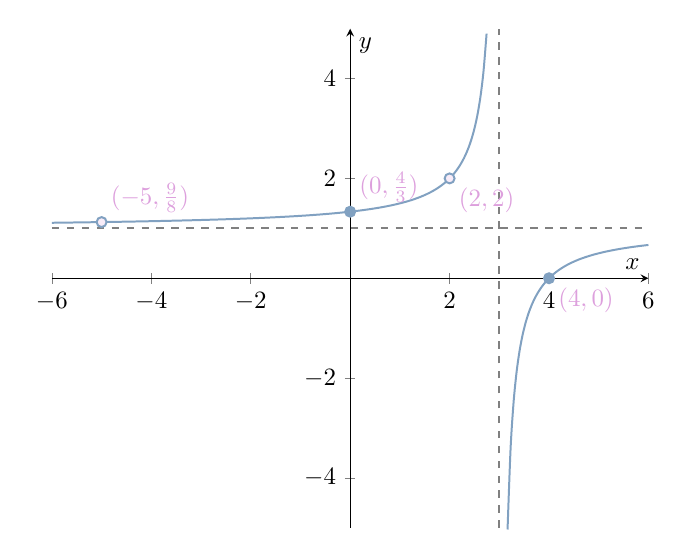
\begin{tikzpicture}[scale=0.9]
        \begin{axis}[xmin=-6, xmax=6, xstep=1, ymin=-5, ymax=5, ystep=1, axis lines=middle, restrict y to domain=-6:6, clip=false, xlabel=\(x\), ylabel=\(y\), every axis plot/.append style={thick}]
            \addplot[color=gray, dashed, domain=-6:6]{1};
            \addplot[color=gray, dashed, samples=50, smooth] coordinates {(3,-5)(3,5)};
            \addplot[color=blue, samples=200, smooth, domain=-6:6]{(x - 4) / (x - 3)};
            \addplot[color=blue, mark=*] coordinates {(4, 0)} node[color=Plum, anchor=north west, pos=1]{\( (4, 0) \)};
            \addplot[color=blue, mark=*] coordinates {(0, 4/3)} node[color=Plum, anchor=south west, pos=1]{\( (0, \frac{4}{3}) \)};
            \addplot[color=blue, fill=examplebg, hole] coordinates {(2, 2)} node[color=Plum, anchor=north west, pos=1]{\( (2, 2) \)};
            \addplot[color=blue, fill=examplebg, hole] coordinates {(-5, 9/8)} node[color=Plum, anchor=south west, pos=1]{\( (-5, \frac{9}{8}) \)};
        \end{axis}
    \end{tikzpicture}
    \end{center}
\end{example}

\section{Continuous Functions and Continuity at Points}

\subsection{Continuity and Types of Discontinuities}

This section tackles the question of when a function is "smooth," or more aptly, continuous, and when it is not.

\begin{definition}{continuous}
    A function \( f \left( x \right) \) is \defterm{continuous} on \( \mathbb{R} \) (in particular \( x = c \)) if and only if all three of these conditions are upheld.
    
    \begin{enumerate}
        \item \( f \left( c \right) \) exists
        \item \( \lim\limits_{x \to c} f \left( x \right) \) exists
        \item \( \lim\limits_{x \to c} f \left( x \right) = f \left( c \right) \)
    \end{enumerate}
    
    Note that a function is continuous if it is continuous at each point of its domain, not necessarily all real numbers. This implies that functions such as \( y = \frac{1}{x} \) are considered continuous despite not existing at \( x = 0 \).
    
    \vspace{0.2cm}
    
    In addition, all polynomial functions are continuous over all real numbers.
\end{definition}

\begin{tip}
    When asked to discuss the continuity of a function, you should state where it is and is not continuous and why. It is not enough to say that the function is continuous on its own domain.
\end{tip}

When one of these three conditions are not upheld at a point, we say that there is a \defterm{discontinuity} at that point. There are several types of discontinuities.

\begin{itemize}
    \item The most important of the discontinuities is the \defterm{removable discontinuity}. This is the "official" name for what we have termed a "hole" in the graph earlier. From now on, you should refer to these discontinuities only as removable discontinuities. Removable discontinuities are discontinuous at only a single point.
    
    \begin{center}
    \begin{tikzpicture}[scale=0.9]
        \begin{axis}[xmin=-2, xmax=2, xstep=1, ymin=-2, ymax=2, ystep=1, axis lines=middle, xlabel=\(x\), ylabel=\(y\), every axis plot/.append style={thick}]
            \addplot[color=blue]{1};
            \addplot[hole, color=blue, fill=bg] coordinates {(1, 1)};
            \addplot[mark=*, color=blue, fill=blue] coordinates {(1, -1)};
        \end{axis}
    \end{tikzpicture}
    \end{center}
    
    \item Another form of discontinuity is the \defterm{infinite discontinuity}, found when there is a vertical asymptote in the function.
    
    \begin{center}
    \begin{tikzpicture}[scale=0.9]
        \begin{axis}[xmin=-2, xmax=2, xstep=1, ymin=-8, ymax=8, ystep=1, axis lines=middle, restrict y to domain=-10:10, xlabel=\(x\), ylabel=\(y\), every axis plot/.append style={thick}]
            \addplot[color=blue, samples=200, smooth, domain=-2:2]{1 / x};
        \end{axis}
    \end{tikzpicture}
    \end{center}
    
    \item \defterm{Jump discontinuities} are also a common discontinuity, seen when the \( y \)-value jumps up or down before continuing on. This appears commonly in the floor and ceiling functions.
    
    \begin{center}
    \begin{tikzpicture}[scale=0.9]
        \begin{axis}[xmin=-2, xmax=2, xstep=1, ymin=-2, ymax=2, ystep=1, axis lines=middle, xlabel=\(x\), ylabel=\(y\), every axis plot/.append style={thick}]
            \addplot[color=blue, domain=-2:1]{-1};
            \addplot[mark=*, color=blue, fill=blue] coordinates {(1, -1)};
            \addplot[hole, color=blue, fill=bg] coordinates {(1, 1)};
            \addplot[color=blue, domain=1:2]{1};
        \end{axis}
    \end{tikzpicture}
    \end{center}
    
    \item Lastly, and the rarest, is the \defterm{oscillating discontinuity}, where the function appears to be approaching multiple values at once, seen in trigonometric functions such as \( y = \sin{\left( \frac{1}{x} \right)} \) when \( x \) approaches \( 0 \).

    \begin{center}
    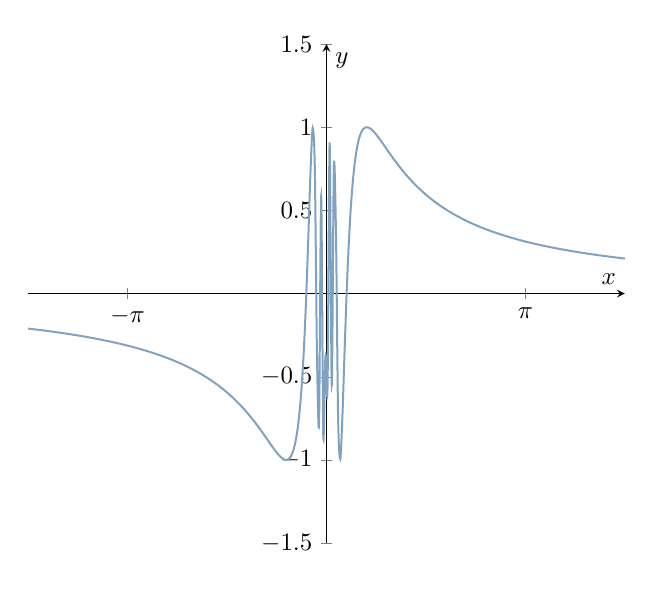
\begin{tikzpicture}[scale=0.9]
        \begin{axis}[
            xmin=-1.5 * pi,
            xmax=1.5 * pi,
            xtick={-pi, pi},
            xticklabels={\( -\pi \), \( \pi \)},
            xticklabel style={anchor=north},
            ymin=-1.5,
            ymax=1.5,
            axis lines=middle,
            xlabel=\(x\),
            ylabel=\(y\),
            every axis plot/.append style={thick}
        ]
            \addplot[color=blue, samples=300, smooth]{sin(deg(1/x))};
        \end{axis}
    \end{tikzpicture}
    \end{center}
\end{itemize}

\subsection{Continuity at Endpoints}

Consider the graph of a function \( y = f \left( x \right) \).

\begin{center}
    \begin{tikzpicture}[scale=0.9]
        \begin{axis}[
            xmin=-2,
            xmax=2,
            xtick={-1, 1},
            xticklabels={\( a \), \( b \)},
            xticklabel style={anchor=north},
            ymin=-2,
            ymax=2,
            axis lines=middle,
            xlabel=\(x\),
            ylabel=\(y\),
            every axis plot/.append style={thick}
        ]
            \addplot[color=blue, domain=-1:1]{1};
            \addplot[hole, color=blue, fill=bg] coordinates {(-1, 1)};
            \addplot[mark=*, color=blue, fill=blue] coordinates {(1, 1)};
        \end{axis}
    \end{tikzpicture}
\end{center}

We can see that at both \( x = a \) and \( x = b \), the function does not continue. When this happens, we call those points \defterm{endpoints}.

\begin{definition}{continuity at endpoints}
    A function is continuous at some endpoint(s) if
    
    \[ \lim_{x \to a^+} f \left( x \right) = f \left( a \right) \]
    \begin{center}
        \textbf{or}
    \end{center}
    \[ \lim_{x \to b^-} f \left( x \right) = f \left( b \right) \]
    
    where \( a \) represents a left endpoint and \( b \) represents a right endpoint.
\end{definition}

\subsection{Removing Discontinuities}

A common exercise that might be asked of you is to locate and remove a discontinuity in a function by rewriting it as a piece-wise function. Sometimes difficulty will arise in identifying where the discontinuity is, while other times it will be evaluating it. Remember to only remove discontinuities if told to do so.

\begin{example}{removing discontinuities}
    The function \( y = \frac{\sin{x}}{x} \) is defined for all real numbers except for \( x = 0 \). If you were asked to remove the discontinuity at \( x = 0 \), thereby making the function continuous, what value would you put in?
    
    Because continuity requires that the limit and the function value must equal, let us take the limit and see what value we need to have at \( x = 0 \).
    
    \[ \lim_{x \to 0} \dfrac{\sin{x}}{x} = 1 \]
    
    So, in order for us to make the function continuous, we should define it to be equal to \( 1 \) at \( x = 0 \). Now that we have this information, we can write our function. Remember to only ever replace discontinuities with number values and to leave the original function otherwise unchanged.
    
    \[
    f \left( x \right) = \begin{cases}
        \dfrac{\sin{x}}{x}, & x \ne 0 \\
        1, & x = 0
    \end{cases}
    \]
\end{example}

Sometimes you will also be tasked with finding out \textit{where} the removable discontinuity is. Questions like this usually involve factoring. Remember, if there is the same zero term in the numerator and denominator, there will likely be a removable discontinuity at that \( x \) value. Just make sure to show your limit work for arriving at that value.

\begin{example}{locating a discontinuity}
    Take a look at the function
    
    \[ y = \dfrac{x^3 - 7x - 6}{x^2 - 9} \]
    
    Locating a discontinuity for a function like this is a clear exercise in factoring.
    
    \[ y = \dfrac{\left( x^2 + 3x + 2 \right) \left( x - 3 \right)}{\left( x - 3 \right) \left( x + 3 \right)} \]
    
    Here, we can see that there is an \( \left( x - 3 \right) \) term in both the numerator and denominator, leading us to believe that there should be a removable discontinuity at \( x = 3 \). To show our work for this, evaluate the limit as \( x \) approaches \( 3 \).
    
    \[ \lim_{x \to 3} \dfrac{\left( x^2 + 3x + 2 \right) \cancel{\left( x - 3 \right)}}{\cancel{\left( x - 3 \right)} \left( x + 3 \right)} = \dfrac{10}{3} \]
    
    Now, we can rewrite our function to be continuous
    
    \[
    f \left( x \right) = \begin{cases}
        \dfrac{x^3 - 7x - 6}{x^2 - 9}, & x \ne 3 \\
        \dfrac{10}{3}, & x = 3
    \end{cases}
    \]
\end{example}

\section{Maximums, Minimums, and Intermediates}

In this section, we'll be able to identify local and global maximum and minimum values and use them in interpreting graphs.

\subsection{Extreme Values}

\begin{theorem}{Min-Max Theorem/Extreme Value Theorem}
    If \( f \) is continuous at every point of a closed interval \( [a, b] \), then \( f \) takes on both a maximum value \( M \) and a minimum value \( m \) somewhere in that interval, and \( m \le f \left( x \right) \le M \) at every other point \( x \) of the interval.
\end{theorem}

This theorem, although worded in a formal way, is quite intuitive. For some continuous function over an interval, there must be a largest and smallest value somewhere in the interval. This can also be seen with a graph.

\begin{center}
    \begin{tikzpicture}[scale=0.9]
        \begin{axis}[
            xmin=-pi,
            xmax=pi,
            xtick={-3 * pi / 4, -pi/2, pi / 2, 3 * pi / 4},
            xticklabels={\( a \), \( x_1 \), \( x_2 \), \( b \)},
            xticklabel style={anchor=north},
            ymin=-1.5,
            ymax=1.5,
            ytick={-1, 1},
            yticklabels={\( m \), \( M \)},
            yticklabel style={anchor=east},
            axis lines=middle,
            xlabel=\(x\),
            ylabel=\(y\),
            every axis plot/.append style={thick}
        ]
            \addplot[color=blue, domain=-3*pi/4:3*pi/4, smooth, samples=200]{sin(deg(x))};
            \addplot[color=Plum, mark=*] coordinates {(-pi/2, -1)} node[anchor=north]{\( \left( x_1, m \right) \)};
            \addplot[color=Plum, mark=*] coordinates {(pi/2, 1)} node[anchor=south]{\( \left( x_2, M \right) \)};
        \end{axis}
    \end{tikzpicture}
\end{center}

Here we see that, in the interval from \( x = a \) to \( x = b \), there is only one minimum point \( \left( x_1, m \right) \) and only one maximum point \( \left( x_2, M \right) \), with all other values of the function between those two numbers.

\subsection{Absolute and Local Extrema}

In Calculus, we make the distinction between absolute, or global, minimums and maximums as opposed to local, or relative, minimums and maximums.

\begin{definition}{absolute minimum/maximum}
    The \defterm{absolute minimum or maximum} is the \textit{one} lowest or highest point of the graph, respectively. If there is a discontinuity at the point in which there should be an absolute extremum, the absolute extremum does not exist.
\end{definition}

\begin{definition}{local minimum/maximum}
    \defterm{Local minimums and maximums} are, as the name would suggest, locally minimal or maximal relative to their surroundings. There can be multiple local extrema in a graph, and local extrema can also be global extrema.
\end{definition}

\begin{example}{absolute and local extrema}
    Let us take a look at some graph \( y = g \left( x \right) \).

    \begin{center}
        \begin{tikzpicture}[scale=0.9]
            \begin{axis}[
                xmin=-0.1,
                xmax=4,
                xticklabels={,,},
                yticklabels={,,},
                ymin=-0.1,
                ymax=2,
                axis lines=middle,
                xlabel=\(x\),
                ylabel=\(y\),
                every axis plot/.append style={thick}
            ]
                \addplot[color=blue, samples=200, domain=-0.1:3.25]{0.25 * sin(3 * deg(x)) + 0.5 * x};
                \addplot[hole, color=purple, fill=examplebg] coordinates {(2.86123643, 1.615700076)} node[color=black, anchor=south]{\( M_a \)};
                \addplot[mark=*, color=blue, fill=blue] coordinates {(0, 0)} node[color=black, anchor=south west]{\( m_a \)};
                \addplot[mark=*, color=blue, fill=blue] coordinates {(0.7668413277, 0.569759662)} node[color=black, anchor=south]{\( M_l \)};
                \addplot[mark=*, color=blue, fill=blue] coordinates {(1.327553775, 0.4774378892)} node[color=black, anchor=south]{\( m_l \)};
                \addplot[mark=*, color=blue, fill=blue] coordinates {(2.86123643, 1.3)};
            \end{axis}
        \end{tikzpicture}
    \end{center}
    
    In this graph, we have an absolute minimum at \( m_a \), and a local minimum at \( m_l \). We also have a local maximum \( M_l \). However, take close note to the discontinuity where the maximum \( M_a \) \textit{should} be. Despite the function being continuous at every other point, because there is no defined largest value, \textbf{the absolute maximum does not exist}.
\end{example}

\subsection{Bounded Functions}

\begin{definition}{bounded function}
    A function \( f \left( x \right) \) is said to be \defterm{bounded above} a value \( c \) if all values of the function are less than or equal to that value \( c \). Similarly, a function \( f \left( x \right) \) is said to be \defterm{bounded below} a value \( c \) if all values of the function are greater than or equal to that value \( c \).
    
    \vspace{0.2cm}
    
    A function is considered \defterm{bounded} when it has \textbf{both} a lower and upper bound.
\end{definition}

\begin{example}{bounded function}
    The function \( y = \sin{x} \) is bounded above by \( y = 1 \) (or any value greater than \( 1 \) as well) and bounded below by \( y = -1 \). From this, we can see that the function \( y = \sin{x} \) is a bounded function.
\end{example}

One use case for this is being able to find an inequality that you can use with the Sandwich Theorem to evaluate a limit. Although this will not be used too often, it is helpful to know the terminology. 

\subsection{Intermediate Values}

\begin{theorem}{Intermediate Value Theorem}
    A function \( y = f \left( x \right) \) that is continuous on a closed interval \( [a, b] \) takes on every value between \( f \left( a \right) \) and \( f \left( b \right) \).
\end{theorem}

This theorem, when deconstructed, is also quite intuitive. If a function does not have any discontinuities, then it must pass through all the values in a given interval. You might also see this phrased as: you can associate at least one \( x \) value in the interval \( [a, b] \) to any \( y \) value in the interval \( [f \left( a \right), f \left( b \right)] \).

\begin{center}
    \begin{tikzpicture}[scale=0.9]
        \begin{axis}[
            xmin=-0.1,
            xmax=2,
            xtick={0.25, pi/4 + 0.25, 0.25 + pi/2},
            xticklabels={\( a \), \( c \), \( b \)},
            xticklabel style={anchor=north},
            ymin=-0.1,
            ymax=1.5,
            ytick={0.479848847066, 0.64352079242, 1.1707354924},
            yticklabels={\( f \left( a \right) \), \( f \left( c \right) \), \( f \left( b \right) \)},
            yticklabel style={anchor=east},
            axis lines=middle,
            xlabel=\(x\),
            ylabel=\(y\),
            every axis plot/.append style={thick}
        ]
            \addplot[color=blue, samples=200, smooth, domain=0.25:0.25 + pi/2]{pow(sin(deg(3 / 2 * x - 7 / 8)), 2) + 1 / 4};
            \addplot[color=blue, mark=*] coordinates {(0.25, 0.479848847066)};
            \addplot[color=blue, mark=*] coordinates {(pi/4 + 0.25, 0.64352079242)};
            \addplot[color=blue, mark=*] coordinates {(0.25 + pi/2, 1.1707354924)};
            
            \addplot[color=gray, dashed] coordinates {(0, 0.479848847066) (0.25, 0.479848847066) (0.25, 0)};
            \addplot[color=blue, dashed] coordinates {(0, 0.64352079242) (pi/4 + 0.25, 0.64352079242) (pi/4 + 0.25, 0)};
            \addplot[color=gray, dashed] coordinates {(0, 1.1707354924) (pi/2 + 0.25, 1.1707354924) (pi/2 + 0.25, 0)};
        \end{axis}
    \end{tikzpicture}
\end{center}

One common exercise involving the IVT is to prove that there exists a \( 0 \) of a function in some interval.

\begin{example}{using the IVT}
    Given the equation
    
    \[ f \left( x \right) = x^3 + x^2 - 4x - 3 \]
    
    Prove that there is a \( 0 \) of the function somewhere in the interval \( [1, 2] \).
    
    \vspace{0.5cm}
    
    Plugging in the bounds of the interval into the function, we get
    
    \begin{align*}
        f \left( 1 \right) &= -5, \\
        f \left( 2 \right) &= 1
    \end{align*}
    
    Combining our knowledge of all polynomial functions being continuous, we can understand that the function should pass through the \( x \)-axis somewhere in the given interval. A full explanation utilizing the theorem would look something like:
    
    \vspace{0.3cm}
    
    "Because \( f \left( x \right) \) is continuous between \( [1, 2] \) it takes on every value between \( -5 \) and \( 1 \). Because \( -5 \le 0 \le 1 \), the function must equal \( y = 0 \) at some point between \( x = 1 \) and \( x = 2 \) by the Intermediate Value Theorem."
\end{example}

\chapter{Derivatives and Rates of Change}

\section{Beginning Derivatives}

\subsection{Introduction}

One of the first concepts that you are introduced to in an algebra class is the concept of slope. When we have two points, \( \left( x_1, y_1 \right) \) and \( \left( x_2, y_2 \right) \), we can find a number that represents the "tilt" of line that passes through both of these points using the formula

\[ m = \dfrac{y_2 - y_1}{x_2 - x_1} \]

You may or may not have also learned that when we apply this formula to some function \( f \left( x \right) \), obtaining the slope between two points, it is called a \defterm{secant line}.

\begin{center}
    \begin{tikzpicture}[scale=.9]
        \begin{axis}[xmin=-5, xmax=5, xstep=1, ymin=-5, ymax=5, ystep=1, axis lines=middle, xlabel=\(x\), ylabel=\(y\), every axis plot/.append style={thick}]
            \addplot[color=blue, samples=100, smooth]{x^2};
            \addplot[color=red, samples=10]{3*x - 2};
            \addplot[color=Plum,mark=*] coordinates {(2, 4)} node[right, pos=1]{\( (2, 4) \)};
            \addplot[color=Plum,mark=*] coordinates {(1,1)} node[right, pos=1]{\( (1, 1) \)};
        \end{axis}
    \end{tikzpicture}
\end{center}

Let us now say that the distance between \( x_1 \) and \( x_2 \) is some value \( h \). Rewriting our terms, we can express this same secant slope using only a few variables.

\begin{align}
    m = \> &\dfrac{f \left( x + h \right) - f \left( x \right)}{\cancel{x} + h - \cancel{x}} \\
    = \> &\dfrac{f \left( x + h \right) - f \left( x \right)}{h}
\end{align}

This gives us the liberty of playing around with the values, \( h \) in particular. When \( h \) increases, the distance between the points increases, and generally the line looks nothing like the function. When we bring the two points together by making \( h \) some \textit{very} small value close to \( 0 \), though, something interesting happens. Our secant line with two points begins to look like a \defterm{tangent line} with only one point of intersection. In addition, the line begins to look much more similar to the function around the point.

\begin{center}
    \begin{tikzpicture}[scale=.9]
        \begin{axis}[xmin=-5, xmax=5, xstep=1, ymin=-5, ymax=5, ystep=1, axis lines=middle, xlabel=\(x\), ylabel=\(y\), every axis plot/.append style={thick}]
            \addplot[color=blue, samples=100, smooth]{x^2};
            \addplot[color=red, samples=10]{2*x - 1};
            \addplot[color=Plum,mark=*] coordinates {(1,1)} node[right, pos=1]{\( (1, 1) \)};
        \end{axis}
    \end{tikzpicture}
\end{center}

This is interesting, but how do we express this very, almost infinitesimally, small value \( h \) mathematically? The answer is simple and is a concept that we have just learned. We need to take the limit as \( h \) approaches \( 0 \).

\begin{definition}{derivative}
    The \defterm{derivative} of a function \( f \) is the function \( f^\prime \) whose value at \( x \) is defined by
    \[ f^\prime \left( x \right) = \lim_{h \to 0} \dfrac{f \left( x + h \right) - f \left( x \right)}{h} \]
    The derivative represents the rate of change, or slope, at a specific point of the function \( f \).
\end{definition}

In addition, the alternative definition of the derivative at a point \( x = c \) is as follows.

\[ f^\prime \left( c \right) = \lim_{x \to c} \dfrac{f \left( x \right) - f \left( c \right)}{x - c} \]

where \( c \) will be a given real number. Only use this when directly specified.

\begin{notation}{derivative}
    Several derivative notations emerged throughout 1700-1800s and were used by various esteemed mathematicians of the time.
    
    \begin{multicols}{2}
    \begin{itemize}
        \item \( \dot y \) from Newton
        \item \( \dfrac{dy}{dx} = \dfrac{df}{dx} = \dfrac{d}{dx} \left( f \right) \) from Leibniz
        \item \( D_x \left( f \right) \) from Arbogast
        \item \( f^\prime \left( x \right) \) from Lagrange
    \end{itemize}
    \end{multicols}
    
    In addition, the partial derivative notation \( \frac{\partial}{\partial x} \) was pioneered by Legendre.
    
    There are also multiple ways of denoting \( n \)th derivatives, or the derivative applied \( n \) times.
    
    \begin{multicols}{2}
    \begin{itemize}
        \item \( \dfrac{d^n}{dx^n} \)
        \item \( y^{\prime \prime} \)
        \item \( f^{(n)} \left( x \right) \)
        \item \( y^{(n)} \left( x \right) \)
    \end{itemize}
    \end{multicols}
    
    While most of these notations are all somewhat relevant, the notations pioneered by Leibniz and Lagrange remain the most commonplace today.
\end{notation}

\begin{example}{derivative notation}
    \begin{align}
        y = x^2 &\implies y^\prime = 2x \\
        y = \sqrt{x} &\implies \dfrac{dy}{dx} = \dfrac{1}{2\sqrt{x}} \\
        y = \dfrac{1}{x} &\implies D_x \left( y \right) = -\dfrac{1}{x^2}
    \end{align}
\end{example}

Once we have a slope, obtained from evaluating the derivative of the function at the point, we can also find the tangent line itself.

\begin{definition}{tangent line}
    The tangent line to a function \( f \left( x \right) \) at a point \( x = a \) is given as follows
    
    \[ y - f \left( a \right) = f^\prime \left( a \right) \left( x - a \right) \]
    
    This represents a line with the same slope as the derivative at that point, intersecting at only one point.
\end{definition}

Although much more uncommon compared to the tangent slope, another related value is the \defterm{normal slope}.

\begin{definition}{normal slope/line}
    The \defterm{normal slope} of a function at a point \( x = a \) is the slope which is perpendicular to the tangent slope. This is expressed as
    
    \[ m_{\text{norm}} = -\dfrac{1}{m_{\text{tan}}} = -\dfrac{1}{f^\prime \left( a \right)} \]
    
    Just like with the tangent line, we can find the \defterm{normal line} to be

    \[ y - f \left( a \right) = -\frac{1}{f^\prime \left( a \right)} \left( x - a \right) \]
\end{definition}

\subsection{Differentiability}

Now that we know \textit{how} to find a derivative, we should also ask: \textit{When} can we find a derivative?

\begin{definition}{differentiable}
    We say that a function is \defterm{differentiable} at a point if we can find the derivative at that point. A function that is differentiable at every point of its domain is called a \defterm{differentiable function}. \par
    
    \vspace{0.3cm}
    
    \textbf{Note}: If a function is differentiable at a point, then it is also continuous at that point. This does \underline{not} imply that the converse, that a function that is continuous at a point is necessarily differentiable at the point, is true, however.
\end{definition}

\textbf{When is a function not differentiable?}

As a consequence of defining the derivative with limits, \textbf{continuity is a requirement for differentiability}. If a function is differentiable, it is also continuous. A function that is continuous, however, need not be differentiable. Consider the following cases.

\begin{itemize}
    \item Functions like \( y = \vert x \vert \) and other similar ones which have a sharp corner or a jump discontinuity in the slope will not have a derivative.
    \item At discontinuities and vertical asymptotes, either the limit or the function will not exist, meaning it will not be differentiable at that point.
    \item At completely vertical tangents, the slope will be infinite or undefined; therefore, the derivative will not exist.
    \item At cusps, which are similar to corners except that they are infinitely sharp, there will be an infinite discontinuity in the derivative, meaning it will not exist at that point.
\end{itemize}

\begin{example}{corner versus cusp}
    Corners and cusps may seem to be almost the same at first glance, but it is important to note their differences in order to differentiate between them.
    
    \vspace{0.3cm}
    
    The graph on the left shows the graph of \( f \left( x \right) = \vert x \vert \) (in {\color{blue} blue}), and its derivative (in {\color{red} red}). This is a \defterm{corner}. Notice the \textit{jump} discontinuity in the derivative.
    
    \vspace{0.3cm}
    
    The graph on the right shows the graph of \( f^\prime \left( x \right) = \sqrt[3]{x^2} \) (in {\color{blue} blue}), and its derivative (in {\color{red} red}). This is an example of a \defterm{cusp}. Notice the \textit{infinite} discontinuity.
    
    \begin{center}
    \begin{tikzpicture}[scale=0.7]
        \begin{axis}[xmin=-2, xmax=2, xstep=1, ymin=-2, ymax=2, ystep=1, axis lines=middle, xlabel=\(x\), ylabel=\(y\), every axis plot/.append style={thick}]
            \addplot[color=blue, samples=20, domain=-2:0]{-x};
            \addplot[color=blue, samples=20, domain=0:2]{x};
            \addplot[color=red, samples=10, domain=-2:0]{-1};
            \addplot[color=red, samples=10, domain=0:2]{1};
            \addplot[hole, color=red, fill=examplebg] coordinates{(0, -1)(0, 1)};
        \end{axis}
    \end{tikzpicture}
    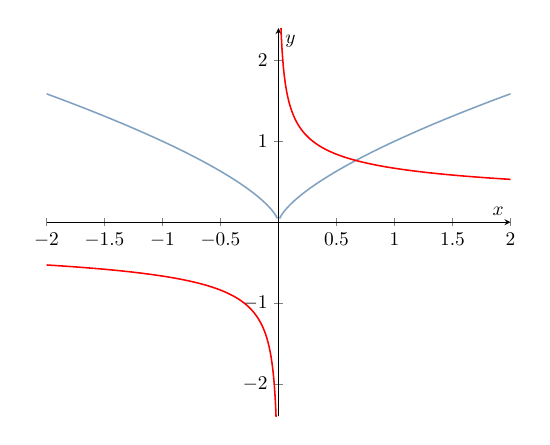
\begin{tikzpicture}[scale=0.7]
        \begin{axis}[xmin=-2, xmax=2, xstep=1, ymin=-2, ymax=2, ystep=1, axis lines=middle, xlabel=\(x\), ylabel=\(y\), enlarge y limits=true, restrict y to domain=-5:5, every axis plot/.append style={thick}]
            \addplot[color=blue, samples=200, smooth, domain=0.01:2]{pow(abs(x), 2/3)};
            \addplot[color=blue, samples=200, smooth, domain=-2:-0.01]{pow(abs(x), 2/3)};
            \addplot[color=red, samples=200, smooth, domain=0:2]{2 / (3 * pow(x, 1/3))};
            \addplot[color=red, samples=200, smooth, domain=-2:0]{2 / (3 * -pow(abs(x), 1/3))};
        \end{axis}
    \end{tikzpicture}
    \end{center}
\end{example}

\begin{example}{differentiable function}
    Consider the function \( f \left( x \right) \). Is it differentiable at \( x = 2 \)?
    \[
    f \left( x \right) = \begin{cases}
            3x - 2 & x < 2 \\
            x^2 & x \ge 2
        \end{cases}
    \]
    
    Using the left-hand limit definition of the derivative
    
    \begin{align}
        &\lim_{h \to 0^-} \dfrac{f \left( 2 + h \right) - f \left( 2 \right) }{h} \\
        = \> &\lim_{h \to 0^-} \dfrac{3 \left( 2 + h \right) - 2 - \left( 2 \right)^2}{h} \\
        = \> &\lim_{h \to 0^-} \dfrac{\cancel{6} + 3\cancel{h} - \cancel{2 - 4}}{\cancel{h}} \\
        = \> &3
    \end{align}
    
    Evaluating the right-hand limit
    
    \begin{align}
        &\lim_{h \to 0^+} \dfrac{f \left(2 + h \right) - f \left( 2 \right)}{h} \\
        = \> &\lim_{h \to 0^+} \dfrac{\left( 2 + h \right)^2 - 2^2}{h} \\
        = \> &\lim_{h \to 0^+} \dfrac{\cancel{2^2} + 4\cancel{h} + h^{\cancel{2}} - \cancel{2^2}}{\cancel{h}} \\
        = \> &4
    \end{align}
    
    Because the left-hand and the right-hand limits are not equal, the derivative does not exist; thus, the function \( f \) is not differentiable at \( x = 2 \).
\end{example}

\section{Derivatives with Calculators}

\subsection{Numeric Derivatives by Graph}

When encountering the terms CAS (computer algebra system) or NDER (numeric derivative), you will need to use a calculator to evaluate the derivatives. \par

Consider the function

\[ f \left( x \right) = \dfrac{2^{x + 1} - \sin{\left( \frac{x + 1}{x - 2} \right)}}{\sqrt[3]{x^3 - 2x + 7}} \]

To find the derivative using your calculator:

\begin{itemize}
    \item On a TI-84: Press \( 2 \)nd \( \to \) Press Trace \( \to \) Press \( \frac{dy}{dx} \)
    \item On a TI-89: Press F5 \( \to \) Press \( \frac{dy}{dx} \)
\end{itemize}

From there, you can use the point and the slope found to write the equation of a tangent line in point-slope form. Here's an example using the function \( f \) from earlier.

\[ y - 0.500 = 0.492 \left( x + 1 \right) \]

\begin{tip}
    Tangent lines can be left in point-slope form; there is no need to convert them to \( y = mx + b \) form on the test.
\end{tip}

For convenience, you can also use the equations that you've graphed as functions.

\begin{itemize}
    \item On a TI-84: Press the \verb+vars+ button \( \to \) Navigate to the heading \verb+Y-VARS+ \( \to \) Go to \verb+Function+ \( \to \) Press \( Y_1 \) (or the corresponding equation that you want the function for).
\end{itemize}

\subsection{Numeric Derivatives by Functions}

Given the function

\[ h \left( x \right) = \ln{\left( x \right)}\sin{\left( x \right)} \]

You may be prompted to find the derivative at some value, for example \( x = 3.2 \). While you can graph this function and find it like previously mentioned, a possibly faster way could be to use the derivative functions on the calculator.

\begin{itemize}
    \item On a TI-84: Go to \verb+math+ \( \to \) Press \verb+nDeriv+ \( \to \) Plug in the values and the variable that you are differentiating with respect to. For finding the derivative of \( h \left( x \right) \) at \( x = 3.2 \), it should look something like this:
    \[ \frac{d}{dx} \left( \ln{\left( x \right)} \sin{\left( x \right)} \right) \vert_{x=3.2} \]
    \item On a TI-89: Press F3 \( \to \) Press the \( d \) button \( \to \) Plug in the function \( \to \) Insert the vertical bar at the end of line and plug in the \( x \) value. For \( h \left( x \right) \) it would something like:
    \[ d \left( \ln{\left( x \right)} * \sin{\left( x \right)}, x \right) \vert_{x=3.2} \]
\end{itemize}

\subsection{Finding Second Derivatives}

Second derivatives are especially useful when finding things like acceleration.

\begin{itemize}
    \item On a TI-84: Nest the derivatives, setting the inner \( x \) equal to the outer \( x \). While a bit convoluted, it works:
    \[ \frac{d}{dx} \left( \frac{d}{dx} \left( \ln{\left( x \right)} \sin{\left( x \right)} \right) \vert_{x=x} \right) \vert_{x=3.2} \]
    \item On a TI-89: Simply add an extra argument to the derivative function with the degree (in this case: \( 2 \)):
    \[ d \left( \ln{\left( x \right)} * \sin{\left( x \right)}, x, 2 \right) \vert_{x=3.2} \]
\end{itemize}

\textbf{Note}: Those with a TI-89 also have the option of omitting the bar. This allows you to see the derivative function itself, which will be especially helpful later in Chapter 3 and Chapter 4.

\textbf{Note}: If you use another calculator type, such as the Nspire or a Casio, good luck :)

\subsection{Graphing Derivatives}

\begin{itemize}
    \item On a TI-84: Enter in the original function in the first equation entry, corresponding to \( y_1 \). From there, you can graph the derivative like usual, which should look like
    \[ \dfrac{d}{dx} \left( y_1 \right) \vert_{x=x} \]
    \item On a TI-89: This is quite similar to the TI-84. Graph the function in \( y_1 \) and then graph the derivative in \( y_2 \). It should look something like
    \[ d \left( y_1 \left( x \right), x \right) \]
\end{itemize}

\subsection{Deriving Numerical Derivatives}

\begin{definition}{Symmetric Difference Quotient}
    You will be asked to find the derivative in the same manner that your calculator finds the numerical derivative. This is the \defterm{Symmetric Difference Quotient}. The NDER function on your calculator uses a small, not infinitesimally though, value \( h \) with the formula
    
    \[ \dfrac{f \left( a + h \right) - f \left( a - h \right)}{2h} \]
    
    to calculate the slope at a point \( x = a \). Essentially, the calculator finds the slope of a secant line over a very small interval.
\end{definition}

If an \( h \) value is not specified in a question, it is assumed to be \( 0.01 \). In addition, there should not be a limit nor variables when using the SDQ.

\begin{example}{Symmetric Difference Quotient}
    Consider the function \( f \left( x \right) = x^2 \) at the point \( x = 3 \). Plugging in the information given, the Symmetric Difference Quotient will look something like
    
    \begin{align}
        &\dfrac{f \left( 3 + 0.01 \right) - f \left( 3 - 0.01 \right)}{2 \left( 0.01 \right)} \\
        = \> &\dfrac{\left( 3.01 \right)^2 - \left( 2.99 \right)^2}{0.02}
    \end{align}
    
    Utilizing the fact that this is a difference of squares
    
    \begin{align}
        &\dfrac{\cancel{\left( 3.01 - 2.99 \right)} \left( 3.01 + 2.99 \right)}{\cancel{0.02}} \\
        = \> &6
    \end{align}
\end{example}

\begin{example}{Symmetric Difference Quotient}
    Consider the function \( y = 3x - 2 \) at the point \( x = 4 \). Similarly to before, we can use the formula to get
    
    \begin{align}
        &\dfrac{f \left( 4.01 \right) - f \left( 3.99 \right)}{0.02} \\
        = \> &\dfrac{3 \left( 4.01 \right) - \cancel{2} - 3 \left( 3.99 \right) + \cancel{2}}{0.02} \\
        = \> &\dfrac{3 \cancel{\left( 4.01 - 3.99 \right)}}{\cancel{0.02}} \\
        = \> &3
    \end{align}
\end{example}

\subsection{Conclusion}

In summary, there are 5 different ways to find the derivative of a function at a point.

\begin{enumerate}
    \item Using the limit definition of the derivative.
    \item Using the alternative definition of the derivative.
    \item Using the NDER functions on your calculator.
    \item Using the grahping function on your calculator.
    \item Using the Symmetric Difference Quotient.
\end{enumerate}

\section{The Shortcuts}

Taking the limit or using the graphing function on your calculator to evaluate derivatives is not always convenient. In addition, you may want a simplified, closed-form function for the derivative. Luckily, there are shortcuts or rules that allow us to find derivatives algebraically.

\subsection{Rules}

\begin{rules}{Constant Rule}
    Because the graph of a constant line is horizontal, the slope is always \( 0 \). This is expressed as
    
    \[ y = k \implies y^\prime = 0, \quad k \in \mathbb{R} \]
\end{rules}

\begin{example}{Constant Rule}
    If \( y = 3 \), then \( y^\prime = 0 \).
\end{example}

\begin{rules}{Power Rule}
    For any function of the form \( y = x^n \), we can multiply the function by \( n \) and subtract \( 1 \) from the power. This is expressed as
    
    \[ y = x^n \implies y^\prime = nx^{n - 1} \]
\end{rules}

\begin{example}{Power Rule}
    For example,
    
    \begin{multicols}{2}
    \begin{itemize}
        \item \( \dfrac{d}{dx} \left( x^2 \right) = 2x \)
        \item \( \dfrac{d}{dx} \left( x^3 \right) = 3x^2 \)
        \item \( \dfrac{d}{dx} \left( 3x^3 \right) = 9x^2 \)
        \item \( \dfrac{d}{dx} \left( x^{100} \right) = 100x^{99} \)
    \end{itemize}
    \end{multicols}
    \vspace{0.1cm}
\end{example}

\begin{rules}{Constant Multiple Rule}
    If a function is multiplied by a constant number, then the derivative of the total function is equal to the constant times the function. This is expressed as
    
    \[ y = k f \left( x \right) \implies y^\prime = k f^\prime \left( x \right) \]
\end{rules}

\begin{example}{Constant Multiple Rule}
    For example, if \( y = 6x^2 \), then \( y^\prime = 6 \cdot 2x = 12 x \).
\end{example}

\begin{rules}{Sum and Difference Rule}
    The derivative of the sum of any number of terms is the same thing as the sum of the derivatives of the individual terms. This is expressed as
    
    \[ y = f \left( x \right) + g \left( x \right) \implies y^\prime = f^\prime \left( x \right) + g^\prime \left( x \right) \]
\end{rules}

\begin{example}{Sum and Difference Rule}
    For example, 
    \begin{align*}
        &\dfrac{d}{dx} \left( x^3 + x^2 + x + 1 \right) \\
        = \> &3x^2 + 2x + 1 + 0 \\
        = \> &3x^2 + 2x + 1
    \end{align*}
\end{example}

\begin{rules}{Product Rule}
    If you take the derivative of the product of two functions, it is equal to the first function times the derivative of the second function plus the second function times the derivative of the first function. This is written as
    
    \[ y = f \left( x \right) g \left( x \right) \implies y^\prime = f \left( x \right) g^\prime \left( x \right) + f^\prime \left( x \right) g \left( x \right) \]
\end{rules}

\begin{example}{Product Rule}
    For example, 
    \begin{align*}
        &\dfrac{d}{dx} \left( \left( x^2 \right) \left( 3x - 2 \right) \right) \\
        = \> &x^2 \left( 3 \right) + 2x \left( 3x - 2 \right) \\
        = \> &3x^2 + 6x^2 - 4x \\
        = \> &9x^2 - 4x
    \end{align*}
\end{example}

\begin{rules}{Quotient Rule}
    When given a rational function, the derivative works in a specific way.
    
    \[ y = \dfrac{f \left( x \right)}{g \left( x \right)} \implies y^\prime = \dfrac{f^\prime \left( x \right) g \left( x \right) - f \left( x \right) g^\prime \left( x \right)}{\left( g \left( x \right) \right)^2 } \]
    
    Note that, when applying the quotient rule, never expand out the denominator.
\end{rules}

\begin{example}{Quotient Rule}
    For an example, take
    
    \[ y = \dfrac{2x + 5}{3x^2 - 4} \]
    
    Then
    
    \begin{align*}
        y^\prime = \> &\dfrac{2 \left( 3x^2 - 4 \right) - 6x \left(2x + 5 \right)}{\left(3x^2 - 4 \right)^2} \\
        = \> &\dfrac{6x^2 - 8 - 12x^2 - 30x}{\left( 3x^2 - 4 \right)^2} \\
        = \> &\dfrac{-6x^2 - 30x - 8}{\left(3x^2 - 4 \right)^2} \\
        = \> &\dfrac{-2 \left(3x^2 + 15x + 4 \right)}{\left(3x^2 - 4 \right)^2}
    \end{align*}
\end{example}

\subsection{Second and Higher Order Derivatives}

Successive derivatives are generally straightforward. Apply differentiation multiple times.

Suppose \( y = x^6 - x^5 + 3x + 2 \), then

\begin{align}
    y^\prime = \> &6x^5 - 5x^4 + 3 \\
    \implies y^{\prime \prime} = \> &30x^4 - 20x^3 \\
    \implies y^{\prime \prime \prime} = \> &120x^3 - 60x^2 \\
    \implies y^{(iv)} = \> &360x^2 - 120x \\
    \implies y^{(v)} = \> &720x - 120 \\
    \implies y^{(vi)} = \> &720 \\
    \implies y^{(vii)} = \> &0 \\
    \implies y^{(viii)} = \> &0 \\
    \vdots
\end{align}

Note that when taking derivatives higher than order three, the prime (\(^\prime\)) symbols in the exponent change to roman numerals.

Also note that we can, theoretically, infinitely differentiate this, which will always evaluate to \( 0 \). This means that there are infinite derivatives of the function.

\begin{tip}
    If, when asked to find \textit{all} derivatives, you list only the first \( n \), you will get \textbf{0 points}. You need to list a general form for the higher order derivatives. In addition to derivatives \( y^\prime \) through \( y^{(vi)} \) above, you will need to write
    
    \[ y^{(n)} = 0, \text{for all } n \ge 7 \]
\end{tip}

\subsection{Finding Horizontal Tangents}

The slope of a horizontal line is always \( 0 \). In addition, the derivative of a function represents the slope of a line. So, in order to find a horizontal tangent, set the derivative of a line to 0.

\begin{example}{Finding a Horizontal Tangent}
    Consider the function \( y = x^2 - 8x + 5 \). Its derivative is the function \( y^\prime = 2x - 8 \). Setting this to 0, we get
    
    \begin{align}
        0 &= 2x - 8 \\
        8 &= 2x \\
        x &= 4
    \end{align}
    
    So the function has a horizontal tangent at \( x = 4 \). If you are asked to find the \textit{point} at which the tangent line is horizontal, plug the found \( x \) value back into the \textbf{original} function, not the derivative. \( 4^2 - 8 \left( 4 \right) + 5 = -11 \), so the point at which there is a horizontal tangent is \( \left(4, -11 \right) \).
\end{example}

\section{Velocity, Acceleration, and Other Derivatives}

When given a function that represents a position or a cost at a specific time or unit, its derivatives have special connotations.

\subsection{Introduction}

The position of an object at a time is usually denoted by some function \( s \left( t \right) \), where \( t \) represents time.

\begin{definition}{velocity}
    \defterm{Velocity}, usually referring to instantaneous velocity, is the \textit{first derivative} of the position function.

    \[ s^\prime \left( t \right) = v \left( t \right) \] 

    In addition, when the velocity changes sign (passes through the \( x \)-axis and goes forward), the direction of the object moving at that velocity changes.
\end{definition}

\begin{example}{velocity}
For example, given the position function \( s \left( t \right) = t^2 \), the velocity function is \( v \left( t \right) = s^\prime \left( t \right) = 2t \).
\end{example}

\begin{definition}{speed}
    Another key term is \defterm{speed}, which is velocity without direction, is defined as

    \[ \text{speed} = \vert v \left( t \right) \vert \]
\end{definition}

\begin{example}{speed}
    For example, if \( v \left( a \right) = -2 \) for some point \( a \), then the speed at that point \( a \) is \( 2 \) units.
\end{example}

\begin{definition}{acceleration}
    \defterm{Acceleration} is the rate of change of velocity, so it is the first derivative of velocity, meaning that it is also the second derivative of position.

    \[ a \left( t \right) = v^\prime \left( t \right) = s^{\prime \prime} \left( t \right) \]
\end{definition}

\begin{example}{acceleration}
    Using the function \( s \left( t \right) = t^2 \) from earlier, \( a \left( t \right) = v^\prime \left( t \right) = 2 \).
\end{example}

While this is not really necessary knowledge, the derivative of acceleration (and thus the third derivative of position) is called \defterm{jerk}, which sounds somewhat funny.

\subsection{Problems Utilizing Derivatives}

\begin{itemize}
    \item \textbf{How do you find the time at which a particle reaches its maximum height given a position function \( s \left( t \right) \)?} If we try visualizing a graph with a maximum and its derivative, it is apparent that, at the maximum, the derivative is equal to \( 0 \). So, in order to solve for the \( t \) at which the function is at its maximum, set the derivative of the position function (the velocity) equal to \( 0 \) and solve for \( t \). Note that this also works for minimums.

    \item \textbf{How do you find a particle's position at the maximum height?} After acquiring the time using the previously mentioned method, you can plug it into the \textit{original} function.

    \item \textbf{How do you find out how long a particle has been in the air?} For this, you can either multiply the time at which the particle is at its maximum by \( 2 \) or find the distance between the two zeroes of the original function.
\end{itemize}

\subsection{Cost and Revenue}

Another common application of derivatives is with cost functions.

The average increase of cost is synonymous with the average rate of change. Given a cost function \( c \left( x \right) \), where \( x \) represents units produced, the average increase of cost is

\[ \dfrac{\Delta c}{\Delta x} \]

\begin{definition}{marginal cost}
    \defterm{Marginal cost} is the estimate of the cost of producing one more unit. To find marginal cost, evaluate the derivative of the cost function at the current \( x \) value.

    \[ \text{Marginal cost} = c^\prime \left( x \right) \]
\end{definition}

\begin{example}{marginal cost}
    For example, suppose that it costs
    
    \[ c \left( x \right) = x^3 - 6x^2 + 15x + 100 \]
    
    to produce \( x \) stoves and you currently make \( 10 \) stoves per day. The marginal cost of producing one more unit would be
    
    \[ c^\prime \left( 10 \right) = 3 \left( 10 \right)^2  - 12 \left( 10 \right) + 15 = 300 - 120 + 15 = 195 \]
    
    Thus, the estimated cost for producing one more stove would be \$195.
\end{example}

Also recalling that revenue is the cost subtracted from the total, or gross, income,

\begin{definition}{marginal revenue}
    \defterm{Marginal revenue} works similarly to marginal cost and is the estimated revenue for producing one more unit. To find it, take the derivative of a revenue function and evaluate it at the point \( x \).

    \[ \text{Marginal revenue} = r^\prime \left( x \right) \]
\end{definition}

\section{Derivatives of Trig Functions}

This section tackles the derivatives of trigonometric functions. Suppose we wanted to find the derivative of a function such as \( y = \sin{x} \).

Using the limit definition,

\begin{align}
    &\lim_{h \to 0} \dfrac{\sin{\left( x + h \right)} - \sin{\left( x \right)}}{h} \\
    = \> &\lim_{h \to 0} \dfrac{\sin{x}\cos{h} + \sin{h}\cos{x} - \sin{x}}{h} \\
    = \> &\lim_{h \to 0} \dfrac{\sin{x} \left( \cos{h} - 1 \right) + \sin{h}\cos{x}}{h} \\
    = \> &\lim_{h \to 0} \dfrac{\sin{x} \left( \cos{h} - 1 \right)}{h} + \lim_{h \to 0} \dfrac{\cancel{\sin{h}} \cos{x}}{\cancel{h}} \\
    = \> &\cancelto{0}{\lim_{h \to 0} \dfrac{-\sin{x}\sin^2{h}}{h \left( \cos{h} + 1 \right)}} + \cos{x} \\
    = \> &\cos{x}
\end{align}

Thus,

\[ \dfrac{d}{dx} \left( \sin{x} \right) = \cos{x} \]

Of course, this is quite cumbersome, so it is recommended to know the trigonometric derivatives by definition.

Similarly to \( \sin{x} \),

\[ \dfrac{d}{dx} \left( \cos{x} \right) = -\sin{x} \]

Now that we have the derivatives of the two fundamental trigonometric functions, we can define the others in terms of them and find their derivatives.

For \( y = \tan{x} \), we can use the quotient rule to get

\begin{align}
    &\dfrac{d}{dx} \left( \dfrac{\sin{x}}{\cos{x}} \right) \\
    = \> &\dfrac{\cos^2{x} + \sin^2{x}}{\cos^2{x}} \\
    = \> &\dfrac{1}{\cos^2{x}} \\
    = \> &\sec^2{x}
\end{align}

For the other three trig functions, similar methods can be used to find the derivatives.

\begin{definition}{trig derivatives}
    
    In total, you need to have these six key trig derivatives memorized.
    
    \begin{multicols}{2}
    \begin{itemize}
        \item \( \dfrac{d}{dx} \left( \sin{x} \right) = \cos{x} \)
        \item \( \dfrac{d}{dx} \left( \cos{x} \right) = -\sin{x} \)
        \item \( \dfrac{d}{dx} \left( \tan{x} \right) = \sec^2{x} \)
        \item \( \dfrac{d}{dx} \left( \csc{x} \right) = -\csc{x}\cot{x} \)
        \item \( \dfrac{d}{dx} \left( \sec{x} \right) = \sec{x}\tan{x} \)
        \item \( \dfrac{d}{dx} \left( \cot{x} \right) = -\csc^2{x} \)
    \end{itemize}
    \end{multicols}
    
    \vspace{0.1cm}
    
\end{definition}

\begin{tip}
    It is sometimes helpful to simplify expressions first by using trigonometric identities before taking the derivative.
    
    Consider the function
    
    \[ y = \cos{x}\sec{x} \]
    
    Although we could use the product rule to find the derivative, a far easier solution is to realize that
    
    \begin{align}
        y = &\cos{x}\sec{x} \\
        = \> &\cancel{\cos{x}} \cdot \dfrac{1}{\cancel{\cos{x}}} \\
        = \> &1
    \end{align}
    
    Then, taking the derivative of a constant,
    
    \[ y^\prime = 0 \]
\end{tip}
\chapter{More Complex Derivatives}

\section{The Chain Rule}

This section tackles the Chain Rule, a fundamental part of evaluating derivatives of more complex, composed functions.

\subsection{Introduction}

Suppose that we were asked to find the derivative of the function

\[ y = \left( 2x + 3 \right)^3 \]

If we haphazardly apply the power rule, this would result in

\[ y = 3 \left( 2x + 3 \right)^2 \]

However, this is clearly \textbf{not} correct. If we expand the original polynomial function and differentiate that, we see that it should be

\begin{align}
    y = \> &\left( 2x + 3 \right)^3 \\
    = \> &\left( 4x^2 + 12x + 9 \right) \left( 2x + 3 \right) \\
    = \> &8x^3 + 36x^2 + 54x + 27 \\
    \implies y^\prime = \> &24x^2 + 72x + 54 \\
    = \> &6 \left( 4x^2 + 12x + 9 \right) \\
    = \> &6 \left( 2x + 3 \right)^2
\end{align}

You may notice that, interestingly, the actual derivative is the incorrect derivative multiplied by the value \( 2 \). You may also recognize that the derivative of the expression inside the parentheses is also \( 2 \). This multiplication of the outside derivative and the inside derivative forms the basis of the Chain Rule, also called the "Outside Inside" Rule.

\begin{definition}{The Chain Rule}
    The derivative of the composition of two (or more) functions is equal to the derivative of the first (with the argument unchanged) multiplied by the derivative of the second. This can be expressed as
    
    \[ \dfrac{d}{dx} \left( f \circ g \right) = f^\prime \left( g \left( x \right) \right) g^\prime \left( x \right) \]
\end{definition}

\begin{example}{Applying the Chain Rule (powers)}
    Consider the function
    
    \[ y = \left( 2x^2 - 5x + 2 \right)^3 \]
    
    While we can apply the power rule, we must also take care to multiply by the derivative of the inside of the function, yielding
    
    \begin{align}
        y^\prime = \> &3 \left( \dfrac{d}{dx} \left( 2x^2 - 5x + 2 \right) \right) \left( 2x^2 - 5x + 2 \right)^2 \\
        = \> &3 \left( 4x - 5 \right) \left( 2x^2 - 5x + 2 \right)^2 \\
        = \> &3 \left( 4x - 5 \right) \left( 2x - 1 \right)^2 \left( x - 2 \right)^2
    \end{align}
\end{example}

This is not only applicable to powers but other functions as well, including trigonometric functions.

\begin{example}{Applying the Chain Rule (trigonometry)}
    Find the derivative of the function
    
    \[ y = \tan{\left( 3x \right)} \]
    
    Here, we can take the derivative of the outside tangent function, being careful not to change the inner angle and then multiply by the derivative of the inner angle.
    
    \begin{align}
        y^\prime = \> &\left( \dfrac{d}{dx} \left( 3x \right) \right) \sec^2{\left( 3x \right)} \\
        = \> &\left( \dfrac{d}{dx} \left( 3x \right) \right) \sec^2{\left( 3x \right)} \\
        = \> &3 \sec^2{\left( 3x \right)}
    \end{align}
\end{example}

\begin{example}{Applying the Chain Rule (combination)}
    Find the derivative of the function
    
    \[ y = \sin^2{\left( 4x \right)} \]
    
    First, it will help clarify the situation to rewrite the function as
    
    \[ y = \left( \sin{4x} \right)^2 \]
    
    Now, we can differentiate using the Chain Rule twice.
    
    \begin{align}
        y^\prime = \> &2 \left( \sin{4x} \right) \left( \dfrac{d}{dx} \left( \sin{4x} \right) \right) \\
        = \> &2 \left( \sin{4x} \right) \left( \cos{4x} \right) \left( \dfrac{d}{dx} \left( 4x \right) \right) \\
        = \> &2 \left( \sin{4x} \right) \left( \cos{4x} \right) \left( 4 \right) \\
        = \> &8\sin{4x} \cos{4x}
    \end{align}
\end{example}

\begin{tip}
    Notice that, whether it be a function or a power, the inner argument does not change when using the Chain Rule. If you find yourself changing the inside of a function or power, you may be doing something wrong.
\end{tip}

\subsection{Another Look: Rates of Change}

To intuit why this happens, let us move from a mathematical context to a more scientific context. Consider a unit of speed such as

\[ \num{3} \> \dfrac{\si{\kilo\meter}}{\si{\minute}} \]

\textbf{How would you manipulate this ratio in order to change it from kilometers per minute to kilometers per hour?} Using our knowledge of the relation between the minute and hour, specifically that \( \SI{60}{\minute} = \SI{1}{\hour} \), we can multiply this rate and cancel units to get

\[ \dfrac{\num{3} \> \si{\kilo\meter}}{\num{1} \> \cancel{\si{\minute}}} \cdot \dfrac{\num{60} \> \cancel{\si{\minute}}}{\num{1} \> \si{\hour}} = \num{180} \> \dfrac{\si{\kilo\meter}}{\si{\hour}} \]

Just like using units, at the heart of Calculus are ratios and rates between values and functions. In fact, the relation between units and elements in Calculus (particularly derivatives and integrals) is what makes Calculus so applicable for physics.

Moving onto a more mathematical example, say that we have the relations

\begin{align*}
    y &= v^2, \\
    v &= \sin{u}, \\
    u &= 5x^2
\end{align*}

and we wish to find \( \frac{d}{dx} \).

Using our knowledge of derivatives, we can find relations or ratios between the individual variables:

\begin{align*}
    \dfrac{dy}{dv} &= 2v, \\
    \dfrac{dv}{du} &= \cos{u}, \\
    \dfrac{du}{dx} &= 10x
\end{align*}

\begin{tip}
    Remember, when using the \( \frac{dy}{dx} \) notation, we are finding the relation of how \( y \) changes \defterm{with respect to} \( x \). Think of the \( d \) as an operator that means "a little bit of."
\end{tip}

Just like how we used units to convert one relation to another, we can do the same here.

\begin{align}
    \dfrac{dy}{dx} = \> &\dfrac{dy}{dv} \cdot \dfrac{dv}{du} \cdot \dfrac{du}{dx} \\
    = \> &\dfrac{dy}{\cancel{dv}} \cdot \dfrac{\cancel{dv}}{\cancel{du}} \cdot \dfrac{\cancel{du}}{dx} \\
    = \> &2v \cdot \cos{u} \cdot 10x \\
    = \> &2 \sin{\left( 5x^2 \right)} \cdot \cos{\left( 5x^2 \right)} \cdot 10x \\
    = \> &20x \sin{\left( 5x^2 \right)}\cos{\left( 5x^2 \right)} \\
\end{align}

This chain of cancelling of the rates of change is where the \textit{Chain} Rule gets its name.

We can also come up with these relations by ourselves, allowing us to see where the Chain Rule or "Outside Inside" shortcut comes from and why it is based on the composition of functions.

\begin{example}{decomposing functions for the Chain Rule}
Consider the function

\[ y = \sin{\left( 7 - 5x \right)} \]

We can introduce a new variable to deconstruct the function into two relations

\[
    y = \sin{u}, \quad u = 7 - 5x
\]

Differentiating these individually, we get

\[
    \dfrac{dy}{du} = \cos{u}, \quad \dfrac{du}{dx} = -5
\]

Once again, we can multiply these rates to cancel, leaving us with

\begin{align}
    \dfrac{dy}{dx} = \> &\dfrac{dy}{du} \cdot \dfrac{du}{dx} \\
    = \> &\dfrac{dy}{\cancel{du}} \cdot \dfrac{\cancel{du}}{dx} \\
    = \> &\cos{u} \cdot -5 \\
    = \> &-5 \cos{\left( 7 - 5x \right)}
\end{align}

\end{example}

\begin{tip}
    Using this verbose form of the Chain Rule is definitely \textbf{not} required, but it is helpful to understand why you are doing the operations that you are, instilling confidence in your answer.
\end{tip}

\subsection{Recognizing Derivatives from Limits}

Another exercise that you may come across will ask you to evaluate a complicated limit such as

\[ \lim_{h \to 0} \dfrac{\tan{\left(3 \left(x + h \right) \right)} - \tan{\left( 3x \right)}}{h} \]

While, theoretically, you could try to use trigonometry and algebra to simplify this, a much faster method would be to notice that this is the limit definition of the derivative of \( y = \tan{3x} \). From here, we can differentiate and arrive much quicker to the answer of \( y^\prime = 3\sec^2{3x} \).

\begin{example}{limits to derivatives}
    Consider the limit
    
    \[ \lim_{h \to 0} \dfrac{\sec{\left( 5x^2 \right)} - \sec{\left( 5 \left( x + h \right)^2 \right)}}{h} \]
    
    Paying careful attention to the minus sign, we can see that this can be rewritten as
    
    \begin{align}
        &\dfrac{d}{dx} \left( -\sec{\left( 5x^2 \right)} \right) \\
        = \> &-10x \sec{\left( 5x^2 \right)} \tan{\left( 5x^2 \right)}
    \end{align}
\end{example}

\section{Implicit Differentiation}

\subsection{Explicit and Implicit Equations}

Up until now, we have been taking the derivatives of \defterm{explicit} equations, or those that directly give you a \( y \) expression.

\begin{example}{explicit equation}
    The function
    
    \[ y = x^2 \]
    
    is an explicit function. We can take the derivative of both sides to get
    
    \[ y^\prime = 2x \]
\end{example}

However, not all equations are in the form \( y = f \left( x \right) \). We call these \defterm{implicit} equations.

\begin{example}{implicit equation}
    The equation for a circle is given as
    
    \[ x^2 + y^2 = 1 \]
    
    Because the \( y \) variable is not isolated, this is an implicit equation.
\end{example}

How do we take the derivative of this?

\defterm{Implicit differentiation} is when you take the derivative of an implicit equation. It is almost exactly similar to normal differentiation in that you take the derivative of both sides.

\begin{example}{implicit differentiation}
    Going back to the equation of the circle, we can take the derivatives of both sides, taking note to use the Chain Rule when differentiating an expression with \( y \) as it is a function of \( x \). From there, we can isolate the value of \( y^\prime \).
    
    \begin{align}
        x^2 + y^2 &= 1 \\
        2x + 2y y^\prime &= 0 \\
        2y y^\prime &= -2x \\
        y^\prime = -\dfrac{\cancel{2}x}{\cancel{2}y} \\
        y^\prime = -\dfrac{x}{y}
    \end{align}
    
    Intuitively, this correlates to a line tangent to the unit circle. If we try and imagine in our head a point on the circle and find a slope with this formula, it does make some sense that the tangent slope would be equal to the negative cotangent value. As \( x \) approaches \( 0 \), so does the slope. This correlates with the top and bottom-most points on the circle having \textit{horizontal} tangent lines. As \( y \) approaches \( 0 \), however, the slope goes to both positive and negative infinity. This correlates to the left and right-most points on a circle having a \textit{vertical} tangent line.
\end{example}

This works based on the same principles of normal differentiation.

Consider how we differentiate

\[ y = x^2 \]

On a lower-level, we can expand out and show all the uses of the Chain Rule. When we take the derivative of the left side, we get a constant multiplied by \( y^\prime \) due to the Chain Rule. The same is found on the right side.

\begin{align}
    \dfrac{d}{dx} \left( y \right) &= \dfrac{d}{dx} \left( x^2 \right) \\
    1 \cdot y^\prime &= 2x \cdot \dfrac{dx}{dx}
\end{align}

However, we can simplify this down, knowing that \( \frac{dx}{dx} \) is simply just \( 1 \).

\begin{example}{implicit differentiation}
    Consider the function
    
    \[ x = y^2 \]
    
    While your first intuition may be to write this as an explicit equation, such as
    
    \[ y = \pm \sqrt{x} \]
    
    However, you cannot differentiate with the addition of the \( \pm \) without turning the function into, well, not a function. Luckily, we can use implicit differentiation instead.
    
    \begin{align}
        \dfrac{d}{dx} \left( x \right) &= \dfrac{d}{dx} \left( y^2 \right) \\
        1 &= 2y y^\prime \\
        \implies y^\prime &= \dfrac{1}{2y}
    \end{align}
\end{example}

\begin{example}{implicit differentiation with trig}
    Find the first derivative of the function
    
    \[ y = \sin{\left( x y \right)} \]
    
    For this example, do not forget to use the Product Rule.
    
    \begin{align}
        \dfrac{d}{dx} \left( y \right) &= \dfrac{d}{dx} \left( \sin{\left( x y \right)} \right) \\
        y^\prime &= \cos{\left( xy \right)} \dfrac{d}{dx} \left( xy \right) \\
        y^\prime &= \cos{\left( xy \right)} \left( xy^\prime + y \right) \\
        y^\prime &= x y^\prime \cos{\left( xy \right)} + y \cos{\left( xy \right)} \\
        y^\prime - xy^\prime \cos{\left( xy \right)} &= y \cos{\left( xy \right)} \\
        y^\prime \left( 1 - x\cos{\left( xy \right)} \right) &= y \cos{\left( xy \right)} \\
        y^\prime &= \dfrac{y \cos{\left( xy \right)}}{1 - x \cos{\left( xy \right)}}
    \end{align}
    
    Remember that all \( y^\prime \) terms must be placed on one side to isolate it.
\end{example}

\subsection{Second Degree Implicit Derivatives}

After obtaining a \( y^\prime \) value, you may be asked to differentiate again. This works the same as normal: apply your differentiation rules and simplify as much as you can. One thing to take note of, however, is that you will usually end up with a \( y^\prime \) term in your derivative. Because we know the value of this, we can substitute it back in with the derivative that we found beforehand. In addition, also look to see if you can substitute your original implicit equation back in.

\begin{example}{second degree implicit differentiation (easy)}
    Returning to our equation of a circle, whose first derivative we already calculated,
    
    \begin{align*}
        x^2 + y^2 &= 1 \\
        y^\prime &= -\dfrac{x}{y}
    \end{align*}
    
    We can find the second derivative by differentiating both sides, taking care to apply the Quotient Rule and Chain Rule correctly.
    
    \begin{align}
        \dfrac{d}{dx} \left( y^\prime \right) &= \dfrac{d}{dx} \left( - \dfrac{x}{y} \right) \\
        y^{\prime \prime} &= -\dfrac{y \frac{d}{dx} \left( x \right) - x \frac{d}{dx} \left( y \right)}{y^2} \\
        &= -\dfrac{y - xy^\prime}{y^2}
    \end{align}
    
    We are not done yet. Notice how there is still a \( y^\prime \) term in the numerator. We know the value of this, so we can substitute it in.
    
    \begin{align}
        &= -\dfrac{y - x \overbrace{\left( -\frac{x}{y} \right)}^{y^\prime}}{y^2} \\
        &= -\dfrac{y + \frac{x^2}{y}}{y^2} \cdot \dfrac{y}{y} \\
        &= -\dfrac{x^2 + y^2}{y^3}
    \end{align}
    
    Let us take a look at the numerator now. This expression is exactly our original equation of the unit circle. This further simplifies, giving us a final answer of
    
    \begin{align}
        y^{\prime\prime} &= -\dfrac{1}{y^3}
    \end{align}
\end{example}

Consider the implicit equation

\[ x^2 + xy + y^2 - 5x = 2 \]

Finding the first derivative is relatively simple, but the hard parts comes when you are asked to evaluate the \textit{second} derivative. It won't be the calculus that is hard, but rather the pure algebra and simplification process.

\begin{tip}
    Before looking at the solution, try this problem yourself in order to gain a better understanding. As with many of the examples in this book, this is chosen to give you a good review of the ideas and concepts that you might potentially see (although you won't see a problem of this difficulty on the test). The best way to learn math is not just by looking, but also by doing.
\end{tip}

To start, let's find our first derivative.

\begin{align}
    \dfrac{d}{dx} \left( x^2 + xy + y^2 - 5x \right) &= \dfrac{d}{dx} \left( 2 \right) \\
    2x + xy^\prime + y + 2yy^\prime - 5 &= 0 \\
    xy^\prime + 2yy^\prime &= -2x - y + 5 \\
    y^\prime \left( x + 2y \right) &= -2x - y + 5 \\
    y^\prime &= \dfrac{-2x - y + 5}{x + 2y}
\end{align}

From here, we can differentiate once more, starting by using the Quotient Rule.

\begin{align}
    \dfrac{d}{dx} \left( y^\prime \right) &= \dfrac{d}{dx} \left( \dfrac{-2x - y + 5}{x + 2y} \right) \\
    y^{\prime \prime} &= \dfrac{\left( x + 2y \right) \frac{d}{dx} \left( -2x - y + 5 \right) - \left( -2x - y + 5 \right) \frac{d}{dx} \left( x + 2y \right) }{\left( x + 2y \right)^2} \\
    &= \dfrac{\left( x + 2y \right) \left( -2 - y^\prime \right) - \left( -2x - y + 5 \right) \left( 1 + 2y^\prime \right) }{\left( x + 2y \right)^2}
\end{align}

From here, you can choose to either expand the terms first or substitute the value of \( y^\prime \). I will choose the former.

\begin{align}
    &= \dfrac{\left( -2x - xy^\prime - 4y - 2yy^\prime \right) - \left( -2x - 4xy^\prime - y - 2yy^\prime + 5 + 10y^\prime \right)}{\left( x + 2y \right)^2} \\
    &= \dfrac{-2x - xy^\prime - 4y - 2yy^\prime + 2x + 4xy^\prime + y + 2yy^\prime - 5 - 10y^\prime}{\left( x + 2y \right)^2}
\end{align}

Now we can cancel some terms out and combine like terms (indicated in colors).

\begin{align}
    &= \dfrac{\cancel{-2x} - \textcolor{blue}{xy^\prime} - \textcolor{darkgreen}{4y} - \cancel{2yy^\prime} + \cancel{2x} + \textcolor{blue}{4xy^\prime} + \textcolor{darkgreen}{y} + \cancel{2yy^\prime} - \textcolor{Plum}{5} - \textcolor{yellow!80!black}{10y^\prime}}{\left( x + 2y \right)^2} \\
    &= \dfrac{\textcolor{blue}{3xy^\prime} - \textcolor{yellow!80!black}{10y^\prime} - \textcolor{darkgreen}{3y} - \textcolor{Plum}{5}}{\left( x + 2y \right)^2} \\
    &= \dfrac{y^\prime \left( 3x - 10 \right) - 3y - 5}{\left( x + 2y \right)^2} \\
\end{align}

Now, we can substitute in the previously obtained value of \( y^\prime \)

\begin{align}
    &= \dfrac{\overbrace{\left( \frac{-2x - y + 5}{x + 2y} \right)}^{y^\prime} \left( 3x - 10 \right) - 3y - 5}{\left( x + 2y \right)^2}
\end{align}

In order to simplify matters and not have a fraction in the numerator, we can now multiply both the top and bottom by \( \left( x + 2y \right) \).

\begin{align}
    &= \dfrac{\left( \frac{-2x - y + 5}{x + 2y} \right) \left( 3x - 10 \right) - 3y - 5}{\left( x + 2y \right)^2} \cdot \dfrac{\left( x + 2y \right)}{\left( x + 2y \right)} \\
    &= \dfrac{\left( -2x - y + 5 \right) \left( 3x - 10 \right) - 3y \left( x + 2y \right) - 5 \left( x + 2y \right)}{\left( x + 2y \right)^3}
\end{align}

We can now expand all of the terms once more and simplify.

\begin{align}
    &= \dfrac{\left( -6x^2 + 20x - 3xy + 10y + 15x - 50 \right) - \left( 3xy + 6y^2 \right) - \left( 5x + 10y \right)}{\left( x + 2y \right)^3} \\
    &= \dfrac{-6x^2 + 20x - 3xy + 10y + 15x - 50 - 3xy - 6y^2 - 5x - 10y}{\left( x + 2y \right)^3}
\end{align}

From here, we can once again cancel and combine like terms.

\begin{align}
    &= \dfrac{-\textcolor{Plum}{6x^2} + \textcolor{yellow!80!black}{20x} - \textcolor{blue}{3xy} + \cancel{10y} + \textcolor{yellow!80!black}{15x} - \textcolor{darkred}{50} - \textcolor{blue}{3xy} - \textcolor{darkgreen}{6y^2} - \textcolor{yellow!80!black}{5x} - \cancel{10y}}{\left( x + 2y \right)^3} \\
    &= \dfrac{-\textcolor{Plum}{6x^2} - \textcolor{blue}{6xy} - \textcolor{darkgreen}{6y^2} + \textcolor{yellow!80!black}{30x} - \textcolor{darkred}{50}}{\left( x + 2y \right)^3} \\
    &= \dfrac{-6 \left( \textcolor{Plum}{x^2} + \textcolor{blue}{xy} + \textcolor{darkgreen}{y^2} - \textcolor{yellow!80!black}{5x} \right) - \textcolor{darkred}{50}}{\left( x + 2y \right)^3}
\end{align}

If you'll pay attention to the inside of the parentheses, the expression contains our original implicit equation:

\[ x^2 + xy + y^2 - 5x = 2 \]

This means that we can replace the expression in the parentheses with the value \( 2 \).

\begin{align}
    &= \dfrac{-6 \left( 2 \right) - 50}{\left(x + 2y \right)^3} \\
    &= \dfrac{-12 - 50}{\left( x + 2y \right)^3} \\
    &= \dfrac{-62}{\left( x + 2y \right)^3}
\end{align}

Finally, we have our answer. Note that this method was certainly not the only way of doing so. You could have started by substituting \( y^\prime \). You could have also left everything factored, only expanding at the very end. All of these methods, assuming that you end up with correct answer in the end, are correct.

\section{Inverse Derivatives}

\subsection{Inverse Functions}

Here is a quick review of inverse functions.

\begin{definition}{inverse function}
    Loosely, an \defterm{inverse function} is a function who maps the \textit{output} of the original function to its \textit{input} and vice versa. We find inverse functions by simply swapping the \( y \) and \( x \) variables in their definition.
\end{definition}

\begin{example}{inverse function}
    Take \( y = \tan{x} \). When we flip the \( y \) and \( x \) variables, we get
    
    \begin{align*}
        x &= \tan{y} \\
        \implies y &= \arctan{x}
    \end{align*}
    
    With our normal function, we can plug in a value and express this as
    
    \[ \tan{\left( \dfrac{\pi}{4} \right)} = 1 \]
    
    When we take the inverse, these mappings flip.
    
    \[ \arctan{\left( 1 \right)} = \dfrac{\pi}{4} \]
\end{example}

\subsection{Inverse Trigonometric Derivatives}

With each of the six important trigonometric functions comes six more almost as equally important \defterm{inverse} functions, which have their own unique derivatives.

\begin{multicols}{2}
\begin{itemize}
    \item \( \dfrac{d}{dx} \left( \arcsin{x} \right) = \dfrac{1}{\sqrt{1 - x^2}}, \abs{x} < 1 \)
    \item \( \dfrac{d}{dx} \left( \arccos{x} \right) = -\dfrac{1}{\sqrt{1 - x^2}}, \abs{x} < 1 \)
    \item \( \dfrac{d}{dx} \left( \arctan{x} \right) = \dfrac{1}{1 + x^2} \)
    \item \( \dfrac{d}{dx} \left( \arccsc{x} \right) = -\dfrac{1}{\abs{x} \sqrt{x^2 - 1}}, \abs{x} > 1 \)
    \item \( \dfrac{d}{dx} \left( \arcsec{x} \right) = \dfrac{1}{\abs{x} \sqrt{x^2 - 1}}, \abs{x} > 1 \)
    \item \( \dfrac{d}{dx} \left( \arccot{x} \right) = -\dfrac{1}{1 + x^2} \)
\end{itemize}
\end{multicols}

An important thing to notice this that \textbf{all inverse co-functions will have a negative sign in their derivative}.

\begin{example}{derivatives with inverse trig functions}
    Find
    
    \[ \dfrac{d}{dx} \left( \arcsin{3x} \right) \]
    
    This is no different from taking the derivative of any other function. We will place the argument where \( x \) appears in the derivative and apply the Chain Rule. Note that the \( x^2 \) in the denominator of the derivative applies to the whole input, which is why we have \( 9x^2 \) in the square root and \textbf{not} \( 3x^2 \).
    
    \begin{align}
        = &\dfrac{1}{\sqrt{1 - 9x^2}} \cdot \dfrac{d}{dx} \left( 3x \right) \\
        = &\dfrac{3}{\sqrt{1 - 9x^2}}
    \end{align}
\end{example}

\begin{notation}{inverse trig functions}
    You will also see the notation
    
    \[ y = \sin^{-1}{x} \]
    
    using a \( -1 \) in the exponent to denote that it is the inverse of the function. This is more prevalent in America, for historical reasons. While either notation works, and you should try and stay consistent with the one you use, just know that there are some things to keep in mind.
    
    \begin{align*}
        \cos^{-1}{x} &\ne \dfrac{1}{\cos{x}} \\
        \sec^{-1}{x} &\ne \dfrac{1}{\cos^{-1}{x}} \\
        \sec^{-1}{x} &= \cos{\left( \dfrac{1}{x} \right)}
    \end{align*}
\end{notation}

How would we go about finding these derivatives by ourselves? The first thing we should do is write these in terms of functions that we know the derivatives of. We can write \( y = \arcsin{x} \) as

\begin{align}
    x &= \sin{y}
\end{align}

From then, we can use implicit differentiation, using the Chain Rule.

\begin{align}
    1 &= y^\prime \cos{y} \\
    \implies y^\prime &= \dfrac{1}{\cos{y}}
\end{align}

However, you will notice that this is not the derivative that we looked at earlier. What we now need to do is write this in terms of \( x \). Knowing that \( x  = \sin{y} \),

\begin{align}
    &= \dfrac{1}{\sqrt{1 - \sin^2{y}}} \\
    &= \dfrac{1}{\sqrt{1 - x^2}}
\end{align}

Now we have our derivative as desired. A similar process can be used to find the other five inverse trig derivatives. This is left as an exercise to the reader.

\begin{example}{more inverse trig derivatives}
    Find the derivative of the expression
    
    \[ \arcsec{\left( 3 \sqrt{x + 1} \right)} \]
    
    Using our memorized derivative and the Chain Rule,
    
    \begin{align}
        = &\dfrac{1}{\abs{3 \sqrt{x + 1}} \sqrt{\left( 3 \sqrt{x + 1} \right)^2 - 1}} \cdot \dfrac{d}{dx} \left( 3 \sqrt{x + 1} \right) \\
        = &\dfrac{1}{\abs{\cancel{3}\sqrt{x + 1}} \sqrt{9x + 8}} \cdot \dfrac{\cancel{3}}{2\sqrt{x + 1}} \\
        = &\dfrac{1}{2 \left( x + 1 \right) \sqrt{9x + 8}}
    \end{align}
    
    Note that we can take away the absolute value for the \( \sqrt{x + 1} \) term because the principle root will always be positive.
\end{example}

\subsection{Derivatives of Inverse Functions}

Suppose we wanted to find the derivative of a function at a point as well as the derivative of the inverse at that same point. Is there some sort of relationship between these values?

Consider the function \( y = x^2 \) at the point \( \left( 2, 4 \right) \). We can find our derivative at that point with relative ease.

\begin{align}
    y &= x^2 \\
    \implies y^\prime &= 2x \\
    \implies y^\prime \left( 2 \right) &= 4
\end{align}

Now we will find the derivative of the inverse. Remember that, in order to find the inverse of a function, we can swap the places of \( x \) and \( y \).

\begin{align}
    x &= y^2 \\
    \implies 1 &= 2y y^\prime \\
    \implies y^\prime &= \dfrac{1}{2y} \\
    \implies y^\prime \left( 2 \right) &= \dfrac{1}{4}
\end{align}

For more clarity, I will attempt another example.

Now consider the function \( y = x^3 - x \) at the point \( \left( 2, 6 \right) \). We can find the derivative to be,

\begin{align}
    y &= x^3 - x \\
    \implies y^\prime &= 3x^2 - 1 \\
    \implies y^\prime \left( 2 \right) &= 11
\end{align}

Then, we can find the inverse function derivative by flipping the variables and differentiating.

\begin{align}
    x &= y^3 - y \\
    \implies 1 &= 3y^2 y^\prime - y^\prime \\
    1 &= y^\prime \left( 3y^2 - 1 \right) \\
    \implies y^\prime &= \dfrac{1}{3y^2 - 1} \\
    \implies y^\prime \left( 2 \right) &= \dfrac{1}{11}
\end{align}

Interestingly, in both cases, the inverse derivative's equation, and thus, value at a point are the reciprocals of the original function's. Why is this?

If we take a look at the derivatives using Leibniz notation, this becomes clearer. Looking at our function, we see that it is a function of \( x \). This means that the derivative is written as

\[ \dfrac{dy}{dx} \]

However, when we switch the variables, we end up with \( x \) being a function of \( y \). This makes the derivative

\[ \dfrac{dx}{dy} \]

If we take the reciprocal of \( dy / dx \), we get \( dx / dy \), which somewhat explains why the relation between these two is as such. This means that, if you so desired, you could find the derivatives of inverses without using implicit differentiation; however, you would still have to rewrite the expression in terms of the independent variable.

One might also see this written as

\[ g^\prime \left( f \left( x \right) \right) = \dfrac{1}{f^\prime \left( x \right)} \]

where \( f \) and \( g \) are inverses functions and functions of \( x \). Several AP test questions have appeared using the above fact, such as the two given below.

\begin{example}{inverse derivative reciprocal rule}
    Given \( g \left( x \right) \) and \( h \left( x \right) \) to be inverse functions and
    
    \[ h \left( x \right) = x^3 - 2x + 3 \]
    
    Find \( g^\prime \left( 2 \right) \).
    
    Applying the relation we just learned earlier, we see that, for some \( x \) where \( h \left( x \right) = 2 \),

    \[ g^\prime \left( 2 \right) = \dfrac{1}{h^\prime \left( x \right)} \]
    
    How do we find when \( h \left( x \right) = 2 \)? There is no other good way than trial and error. Luckily, because this is on the test, we know that it will be relatively easy to find by plugging in some small number. After testing some values, we see that \( h \left( 1 \right) = 2 \implies x = 1 \). This lets us plug in \( x = 1 \) to the derivative of \( h \), which we do know how to find.
    
    \begin{align}
        h^\prime \left( x \right) &= 3x^2 - 2 \\
        \implies h^\prime \left( 1 \right) &= 1 \\
        \implies g^\prime \left( 2 \right) &= \dfrac{1}{1} = 1
    \end{align}
\end{example}

\begin{example}{inverse derivative reciprocal rule}
    Given  \( g \left( x \right) \) and \( h \left( x \right) \) to be inverse functions and the following table of values, find \( h^\prime \left( 3 \right) \).
    
    \begin{center}
    \begin{tabular}{c|c|c|c}
        \( x \) & \( g \left( x \right) \) & \( h \left( x \right) \) & \( g^\prime \left( x \right) \) \\
        \hline
        \( 3 \) & \( 5 \) & \( 4 \) & \( -1/4 \) \\
        \( 4 \) & \( 3 \) & \( 1 \) & \( 1/2 \)
    \end{tabular}
    \end{center}
    
    Again using the previous relation between inverse function derivatives, this problem is quite trivial.
    
    \[ h^\prime \left( 3 \right) = \dfrac{1}{g^\prime \left( x \right)} \]
    
    where \( x \) is the value at which \( g \left( x \right) = 3 \). Consulting the table, we see that \( g \left( x \right) = 3 \) when \( x = 4 \). Now looking at the last column, we see that \( g^\prime \left( 4 \right) = 1/2 \). Thus,
    
    \begin{align}
        h^\prime \left( 3 \right) = \dfrac{1}{1/2} = 2
    \end{align}
\end{example}

\section{Natural Logarithms and Exponential Functions}

\subsection{Reviewing Logarithms and Exponentials}

Logarithmic and exponential functions have special rules and relationships that make them especially useful as well as interesting.

For logarithms,

\begin{multicols}{2}
    \begin{itemize}
        \item \( \ln{ab} = \ln{a} + \ln{b} \)
        \item \( \ln{\frac{a}{b}} = \ln{a} - \ln{b} \)
        \item \( \ln{a^b} = b \ln{a} \)
        \item \( \ln{\frac{1}{a}} = \ln{a^{-1}} = -\ln{a} \)
    \end{itemize}
\end{multicols}

In addition, the logarithm of any base \( b \) can be written in terms of the natural logarithm with

\[ \log_a{x} = \dfrac{\ln{x}}{\ln{a}} \]

This will be helpful when taking the derivative of logarithms with different bases.

For exponential functions,

\begin{multicols}{2}
    \begin{itemize}
        \item \( e^{ab} = \left( e^a \right)^b \)
        \item \( e^{a - b} = \dfrac{e^a}{e^b} \)
        \item \( e^{a + b} = e^a \cdot e^b \)
        \item \( e^{-a} = \dfrac{1}{e^a} \)
    \end{itemize}
\end{multicols}

Remember also that \( \ln{x} \) (log base \( e \)) and \( e^x \) are inverse functions. This means that

\[ e^{\ln{x}} = \ln{e^x} = x \]

\( e \), also called Euler's number, is a very special constant, roughly equal to \( 2.7183 \), associated with exponential growth.

This is what the graph of \( y = \ln{x} \) looks like.

\begin{center}
    \begin{tikzpicture}[scale=.9]
        \begin{axis}[xmin=-1, xmax=5, xstep=1, ymin=-3, ymax=3, ystep=1, axis lines=middle, xlabel=\(x\), ylabel=\(y\), restrict y to domain=-100:10, every axis plot/.append style={thick}]
            \addplot[color=blue, samples=150, smooth, domain=0:5]{ln(x)};
            \addplot[mark=*, color=blue, fill=blue] coordinates {(1, 0)} node[anchor=south]{\( \left( 1, 0 \right) \)};
            \addplot[mark=*, color=blue, fill=blue] coordinates {(2.71828, 1)} node[anchor=south]{\( \left( e, 1 \right) \)};
        \end{axis}
    \end{tikzpicture}
\end{center}

Remember that \( \ln{x} \) is not defined for the real numbers in the interval \( \left( -\infty, 0 \right] \). This occurs as a consequence of being the inverse of the exponential function.

From this graph we can see the following limits.

\begin{align*}
    \lim_{x \to 0^+} \ln{\left(x \right)} &\to -\infty \\
    \lim_{x \to \infty} \ln{\left( x \right)} &\to \infty
\end{align*}

\newpage

This is what the graph of \( y = e^x \) looks like.

\begin{center}
    \begin{tikzpicture}[scale=.9]
        \begin{axis}[xmin=-5, xmax=5, xstep=1, ymin=-1, ymax=10, ystep=1, axis lines=middle, xlabel=\(x\), ylabel=\(y\), every axis plot/.append style={thick}]
            \addplot[color=blue, samples=100, smooth]{e^x};
            \addplot[mark=*, color=blue, fill=blue] coordinates {(0, 1)} node[anchor=west]{\( \left( 0, 1 \right) \)};
            \addplot[mark=*, color=blue, fill=blue] coordinates {(1, 2.71828)} node[anchor=west]{\( \left( 1, e \right) \)};
        \end{axis}
    \end{tikzpicture}
\end{center}

From this graph, we can see the following end behavior limits:

\begin{align*}
    \lim_{x \to -\infty} e^x &= 0 \\
    \lim_{x \to \infty} e^x &\to \infty
\end{align*}

\subsection{Logarithmic Derivatives}

The derivative of \( \ln{x} \) is given as follows (for those curious as to why, a proof will be given in Chapter 9). As for all other functions, the Chain Rule still applies.

\[ \dfrac{d}{dx} \left( \ln{x} \right) = \dfrac{1}{x} \]

In fact, the same is true for \( y = \ln{ax} \).

\begin{align}
    &\dfrac{d}{dx} \left( \ln{ax} \right) \\
    = &\dfrac{1}{ax} \cdot \dfrac{d}{dx} \left( ax \right) \\
    = &\dfrac{\cancel{a}}{\cancel{a}x} \\
    = &\dfrac{1}{x}
\end{align}

Another way to verify these derivatives is to use logarithm rules to simplify.

\begin{align}
    &\dfrac{d}{dx} \left( \ln{ax} \right) \\
    = &\dfrac{d}{dx} \left( \ln{a} + \ln{x} \right) \\
    = &\dfrac{1}{x}
\end{align}

\begin{tip}
    Remember, the natural logarithm of any constant value is also a constant. When taking the derivative, it will always evaluate to \( 0 \).
\end{tip}

\begin{example}{simple logarithm derivatives}
    Given the function
    
    \[ y = \ln{x^2} \]
    
    Find \( y^\prime \).
    
    \vspace{0.3cm}
    
    This problem can be tackled in two different ways. Firstly, let's use the Chain Rule with our definition of the derivative.
    
    \begin{align}
        y^\prime &= \dfrac{1}{x^2} \cdot \dfrac{d}{dx} \left( x^2 \right) \\
        &= \dfrac{1}{x^{\cancel{2}}} \cdot 2\cancel{x} \\
        &= \dfrac{2}{x}
    \end{align}
    
    Alternatively, we can simplify with logarithm rules first.
    
    \begin{align}
        y &= 2 \ln{x} \\
        \implies y^\prime &= \dfrac{2}{x}
    \end{align}
    
    Use whichever method you prefer, so long as it is mathematically correct and gives you the correct answer.
\end{example}

\begin{example}{nested logarithmic derivatives}
    If your teacher is feeling especially evil one day, they may ask you to find the derivative of
    
    \[ y = \ln{\left( \ln{\left( \ln{\left( x\right)} \right)} \right)} \]
    
    But, with your knowledge of derivatives, you'll show them who's boss (spoiler alert: it's still them).
    
    \vspace{0.2cm}
    
    \textit{Ahem}, anyways, this is an exercise in applying the Chain Rule.
    
    \begin{align}
        y^\prime &= \dfrac{1}{\ln{\left( \ln{\left( x \right)}\right)}} \cdot \dfrac{d}{dx} \left( \ln{\left( \ln{\left( x \right)}\right)} \right) \\
        &= \dfrac{1}{\ln{\left( \ln{\left( x \right)}\right)}} \cdot \dfrac{1}{\ln{\left( x \right)}} \cdot \dfrac{d}{dx} \left( \ln{\left( x \right)} \right) \\
        &= \dfrac{1}{\ln{\left( \ln{\left( x \right)}\right)}} \cdot \dfrac{1}{\ln{\left( x \right)}} \cdot \dfrac{1}{x} \\
        &= \dfrac{1}{x \ln{\left( x \right)} \ln{\left( \ln{\left( x \right)} \right)}}
    \end{align}
    
    That's a lot of logs.
\end{example}

\subsection{Logarithms of Different Bases}

Remembering back to Pre-Calculus, logarithms can have different bases. For example \( \log_2{2^4} = 4 \) represents a logarithm in base \( 2 \). We don't know how to take the derivatives of these, but luckily we can use the change of bases formula to rewrite this in terms of natural logarithms.

\begin{align}
    &\dfrac{d}{dx} \left( \log_a{x} \right) \\
    = &\dfrac{d}{dx} \left( \dfrac{\ln{x}}{\ln{a}} \right) \\
    = &\dfrac{1}{x} \cdot \dfrac{1}{\ln{a}} \\
    = &\dfrac{1}{x \ln{a}}
\end{align}

Different base logarithm derivative are simply just a constant term away from the natural logarithm derivative. This general form should be memorized.

\begin{example}{log 10 derivative}
    Find the derivative of the function
    
    \[ y = \log_{10}{\left( x^2 + 1 \right)} \]
    
    \vspace{0.3cm}
    
    The derivative of this is the same as it would be for the natural logarithm with an extra constant tacked on.
    
    \begin{align}
        y^\prime &= \dfrac{1}{x^2 + 1} \cdot \dfrac{1}{\ln{10}} \cdot \dfrac{d}{dx} \left( x^2 + 1 \right) \\
        &= \dfrac{1}{\left( x^2 + 1 \right) \ln{10}} \cdot 2x \\
        &= \dfrac{2x}{\left( x^2 + 1 \right) \ln{10}}
    \end{align}
\end{example}

\subsection{Logarithmic Differentiation}

\begin{definition}{log diff}
    \defterm{Logarithmic differentiation}, often shortened to \defterm{log diff}, is the strategy of taking the logarithm of both sides of an equation and taking the derivative, oftentimes converting a explicit differentiation problem to an implicit one.
\end{definition}

To illustrate what this means, let's look an at example.

Consider the familiar function \( y = x^2 \). While we know how to take the derivative normally, we can also show this with log diff. Firstly, we apply the natural log on both sides.
    
\begin{align}
    \ln{y} &= 2 \ln{x}
\end{align}

Now this is an implicit differentiation problem. When taking the derivative, don't forget to apply the Chain Rule.

\begin{align}
    \dfrac{y^\prime}{y} &= \dfrac{2}{x} \\
    y^\prime &= y \cdot \dfrac{2}{x}
\end{align}

You will notice that this is not the derivative we are familiar with, but we can substitute the value of \( y \) back into the equation and simplify further.

\begin{align}
    &= x^{\cancel{2}} \cdot \dfrac{2}{\cancel{x}} \\
    &= 2x
\end{align}

This, however, is a somewhat contrived example. If we already know how to take the derivative normally, and this simply does the same thing with more steps, \defterm{why and when would we use log diff?}

The answer to this is relatively simple, log diff is useful when taking derivatives of functions that can be simplified with logarithm rules and would otherwise be hard or impossible to take the derivative of without.

Consider the extremely fast-growing function \( y = x^x \). We {\color{red} \underline{\textbf{cannot}}} simply apply the Power Rule and say that the derivative is \( y^\prime = x \cdot x^{x - 1} = x^x \) because this would be incorrect. The Power Rule, which can be proven using log diff, only applies for constant powers. To find this derivative correctly, we must use log diff. It is because of logarithmic rules that we can simplify and take the derivative of this.

\begin{align}
    \ln{y} &= x \ln{x} \\
    \implies \dfrac{y^\prime}{y} &= x \cdot \frac{d}{dx} \left( \ln{x} \right) + \ln{x} \cdot \frac{d}{dx} \left( x \right) \\
    \dfrac{y^\prime}{y} &= \cancel{x} \cdot \frac{1}{\cancel{x}} + \ln{x} \cdot 1 \\
    \dfrac{y^\prime}{y} &= 1 + \ln{x} \\
    y^\prime &= y \left( \ln{x} + 1 \right) \\
    &= x^x \left( \ln{x} + 1 \right)
\end{align}

This is the one, true derivative of \( x^x \).

Another place where logarithm rules come in handy is with multiplied and divided polynomials. Note that you can only use this if you are not required to simplify the answer. Consider the function

\[ y = \dfrac{\left( x - 1 \right)^2 \left( 2x + 3 \right)^3}{\left( 5x - 2 \right)^2} \]

When we take the natural logarithm of both sides, we can bring the powers down from the exponent and turn the multiplications and divisions into additions and subtractions, which are much more friendly for differentiation.

\begin{align}
    y^\prime &= 2 \ln{\left( x - 1 \right)} + 3 \ln{\left( 2x + 3 \right)} - 2 \ln{\left( 5x - 2 \right)}
\end{align}

Now we can differentiate, taking care not to forget the Chain Rule.

\begin{align}
    \dfrac{y^\prime}{y} &= \dfrac{2}{x - 1} + \dfrac{6}{2x + 3} - \dfrac{10}{5x - 2} \\
    y^\prime &= y \left( \dfrac{2}{x - 1} + \dfrac{6}{2x + 3} - \dfrac{10}{5x - 2} \right) \\
    y^\prime &= \dfrac{\left( x - 1 \right)^2 \left( 2x + 3 \right)^3}{\left( 5x - 2 \right)^2} \left( \dfrac{2}{x - 1} + \dfrac{6}{2x + 3} - \dfrac{10}{5x - 2} \right)
\end{align}

Once again, though, this is only an acceptable answer if the problem states that you do not have to simplify fully.

\subsection{Exponential Derivatives}

The inverse of the the natural logarithm is the function \( y = e^x \), also denoted as \( \exp{\left( x \right)} \) in some contexts. As these functions are inverses, they go hand-in-hand.

Using our new tool of log diff, we can find the derivative of \( e^x \) ourselves. Logarithmic differentiation lends itself especially well here because of the \( x \) term in the exponent that would otherwise be impossible to deal with.

Setting \( y = e^x \), we can nicely take the natural logarithm of both sides.

\begin{align}
    \ln{y} &= x
\end{align}

Taking the derivative,

\begin{align}
    \dfrac{y^\prime}{y} &= 1 \\
    y^\prime &= y \\
    y^\prime &= e^x
\end{align}

Nope, we did not do that incorrectly. The derivative of \( e^x \) is simply just itself. Its velocity, acceleration, acceleration's acceleration, and so on are all \( e^x \), meaning that it \textbf{grows proportionally to itself}. This is the reason why exponential functions grow so quickly and why things like epidemic outbreaks are modeled by exponential functions. It is not possible to overstate how cool this is, but I only have so much time and energy to write, so I encourage you to look more into this topic outside of class.

A more general form for the derivative of \( y = a^x \) can be found to be

\[ y^\prime = a^x \ln{a} \]

This can be proven with the same methods as previously and should be memorized as well.

\begin{example}{exponential derivatives}
    Find the first derivative of the function
    
    \[ y = 2^{\sin{x}} \]
    
    \vspace{0.3cm}
    
    This is considerably easier than it looks. The great thing about taking the derivative of exponential functions is that you can simply duplicate the function and apply the Chain Rule, remembering to multiply by the constant as well.
    
    \begin{align}
        y^\prime &= 2^{\sin{x}} \cdot \dfrac{d}{dx} \left( \sin{x} \right) \cdot \ln{2} \\
        &= \ln{2} \cdot \cos{x} \cdot 2^{\sin{x}}
    \end{align}
    
    This answer cannot be simplified further.
\end{example}

\chapter{Applications of Derivatives}

\section{Extreme Values of Functions}

\subsection{Critical and Stationary Points}

When finding extrema of functions, which will come up quite soon, it is important to keep in two key definitions.

\begin{definition}{critical and stationary points}
    A \defterm{critical point} is a point in which, given a function \( f \left( x \right) \) and a point \( x \), either \( f^\prime \left( x \right) = 0 \) or \( f^\prime \left( x \right) \) does not exist.
    
    \vspace{0.3cm}
    
    A \defterm{stationary point} is similar, but not entirely the same, when compared to a critical point. Given a function \( f \left( x \right) \) and a point \( x \), that point \( x \) is considered a stationary point when \( f^\prime \left( x \right) = 0 \) on the interior of the domain.
\end{definition}

While the terminology "stationary" is relatively novel, it will be used in your Pearson homework, so it is essential to know.

We look at critical points to see possible changes in the sign of the derivative, or growth of the function, just as we would for critical values with inequalities. Critical points \textit{can} be extrema, but they do not have to be. Similarly, while endpoints also count as local minima and maxima, they are not usually considered critical points.

One tool that utilizes critical points is called the \defterm{sign chart}. This chart allows us to view a function's behavior without needing to graph it.

Suppose we have a function whose critical points are located at \( x = 1 \) and \( x = 3 \), given by
    
\begin{align*}
    f \left( x \right) &= x^3 - 6x^2 + 9x + 2 \\
    f^\prime \left( x \right) &= 3 \left( x - 1 \right) \left( x - 3 \right)
\end{align*}
    
By testing values between the critical points, we can look at the \textit{sign} of the derivative in those intervals. This allows us to view where a function is increasing and decreasing and where potential extrema may be.
    
Simply plugging in values around the critical points, we see
    
\begin{align*}
    f^\prime \left( 0 \right) &= 9 \\
    f^\prime \left( 2 \right) &= -3 \\
    f^\prime \left( 5 \right) &= 24 \\
\end{align*}
    
Looking at the signs of the numbers, we can construct a sign chart now.
    
\begin{figure}[H]
    \centering
    \includesvg[width=300pt]{Figures/SignChart.svg}
\end{figure}
    
Because the derivative is positive on the intervals \( \left( -\infty, 1 \right) \) and \( \left( 3, \infty \right) \), we can see that the function will keep increasing on those intervals. Likewise, \( f^\prime \left( x \right) \) is negative in the interval \( \left(1, 3 \right) \). This means that the function will decrease on that interval. Although we don't know the exact graph or shape of the function, we can see that from our sign chart that the function will have a local \textit{maximum} at \( x = 1 \) and a local \textit{minimum} at \( x = 3 \).

\begin{tip}
    Note: Although the sign chart can be a useful tool, it is \textbf{not} a substitute for an actual explanation on the AP Test. If a problem asks you to describe the interval on which a function is increasing (or something similar), you \textbf{must} write out a sentence explanation.
\end{tip}

\subsection{Locating Extrema}

If you'll remember back to Chapter 2, we learned how to identify absolute and local maxima and minima, or \defterm{extrema}, but we did not cover locating them given a function. Now that we have the power of derivatives, however, we are now able to do this with ease.

Given a function \( f^\prime \left( x \right) \) and an interval over which it is defined, we can find extrema by considering all critical points \textit{and} endpoints. Critical points can be found by setting the derivative to \( 0 \) or when the derivative is undefined. The endpoints can also be found quite easily by plugging in both the values in the interval given.

We can do this as a consequence of the following theorem.

\begin{theorem}{First Derivative Theorem for Local Extrema}
    If a function has a local minimum or maximum at an interior point \( c \) in its domain, and if \( f^\prime \) exists at \( c \), then \( f^\prime \left( c \right) = 0 \).
\end{theorem}

Intuitively, this makes sense. Consider the following sketch

\begin{figure}[H]
    \centering
    \includesvg[width=400pt]{Figures/FDTheoremGraph.svg}
\end{figure}

When an extrema is located at a cusp or a corner of some kind, the derivative does not exist and we cannot find it by setting the derivative to \( 0 \). All other extrema, however, will have horizontal tangent lines. This means that we can find these points by setting the derivative to \( 0 \).

\vspace{0.3cm}

After locating all the points needed, we can construct a table of values and compare them to see which points are maximum and minimum values. This allows us to not only pick out local extrema, but absolute extrema as well.

\begin{example}{locating extrema of a function}
    Consider the function
    
    \[ y = \dfrac{1}{x} + \ln{x} \]
    
    over the interval \( \left[\frac{1}{2}, 4 \right] \). How can we find the extrema?
    
    \vspace{0.3cm}
    
    Just like stated earlier, we can set the derivative to \( 0 \) and solve.
    
    \begin{align}
        y^\prime &= -\dfrac{1}{x^2} + \dfrac{1}{x} \\
        0 &= -\dfrac{1}{x^2} + \dfrac{1}{x}
    \end{align}
    
    From here, we can see that our only critical point is located at \( x = 1 \). Including the endpoint values that we have to check, we can construct a table of values.
    
    \begin{center}
    \begin{tabular}{c|l}
        \( x \) & \( y \) \\
        \hline
        \( 1 \) & \( 1 - \ln{1} = 1 \) \\
        \( 1 / 2 \) & \( 2 - \ln{2} \approx 1.307 \) \\
        \( 4 \) & \( 1/4 + \ln{4} \approx 1.636 \)
    \end{tabular}
    \end{center}
    
    Thus, we can see that there is a local minimum at \( x = 1 \) and two local maxima at \( x = 1/2 \) and \( x = 4 \). In addition, because it has the smallest \( y \) value, the absolute minimum is also located at \( x = 1 \). Similarly, the absolute maximum is located at \( x = 4 \) because it has the largest \( y \) value.
\end{example}

\section{The Mean Value Theorem and So Much More}

\subsection{Mean Value and Rolles' Theorem}

One highly important and iconic theorem in Calculus is the Mean Value Theorem.

\begin{theorem}{Mean Value Theorem}
    If \( y = f \left( x \right) \) is continuous at every point in \( \left[a, b \right] \) and differentiable at every point on the interior \( \left(a, b \right) \), there exists at least one \( c \) between \( a \) and \( b \) in which
    
    \[ f^\prime \left( c \right) = \dfrac{f \left( b \right) - f \left( a \right)}{b - a} \]
\end{theorem}

In reality, all this is stating is that, there is at least one point in which the instantaneous rate of change equals the average rate of change. Intuitively, this makes sense. If all rates of change were below the average rate of change, then the average rate of change would not be the average.

Note also that when using this theorem, you must fulfill the conditions of continuity and differentiability that it states. Some problems will also only state that a function is differentiable over an interval, which would imply that it is continuous on that interval as well.

\begin{example}{using the MVT}
    The function \( f \left( x \right) = x^2 + 3 \) is continuous on \( \left[0, 4 \right] \) and differentiable on \( \left(0, 4 \right) \). Since \( f \left( 0 \right) = 3 \) and \( f \left( 4 \right) = 19 \), the MVT guarantees a point \( c \) in the interval \( \left[0, 4 \right] \) for which 
    
    \[ f^\prime \left( c \right) = \dfrac{f \left( b \right) - f \left( a \right)}{b - a} \]
    
    For what value \( c \) is this true?
    
    \vspace{0.3cm}
    
    Plugging in our values, we can first find the average rate of change and then solve for the value at which the derivative is equal to it.
    
    \begin{align}
        f^\prime \left( c \right) &= \dfrac{19 - 3}{4 - 0} \\
        &= 4 \\
        f^\prime \left( x \right) &= 2x \\
        \implies 2c &= 4 \\
        \implies c &= 2
    \end{align}
\end{example}

Another famous theorem that goes along with the MVT is Rolles' Theorem.

\begin{theorem}{Rolles' Theorem}
    Suppose \( y = f \left( x \right) \) is continuous on \( \left[a, b \right] \) and differentiable at every point on \( \left(a, b \right) \). If \( f \left( a \right) = f \left( b \right) = 0 \), then there exists at least one \( c \) \textit{s.t.} \( f^\prime \left( c \right) = 0 \)
\end{theorem}

This theorem also makes quite a bit of sense. If we have two points with the same \( y \) value, there is always at least one extrema between them or simply just a straight line, both of which have derivatives equal to \( 0 \).

\subsection{Increasing and Decreasing Intervals}

As we've seen before, another prevalent application of derivatives is to find when a function is increasing and decreasing.

\begin{theorem}{first derivative test for increasing and decreasing}
    The original equation \( f \left( x \right) \) is increasing on \( \left[a, b \right] \) when \( f^\prime \left( x \right) > 0 \) on \( \left(a, b \right) \) and decreasing on \( \left[a, b \right] \) when \( f^\prime \left( x \right) < 0 \) on \( \left(a, b \right) \).
\end{theorem}

With very little effort, we can also see that the converse of this, that a function which is increasing on an interval has a positive derivative over all points in that interval, is true.

\begin{example}{intervals of increasing and decreasing}
    Consider the function
    
    \[ y = x^2 \]
    
    When is it increasing and when it is decreasing?
    
    \vspace{0.3cm}
    
    Like usual, we can set the derivative equal to \( 0 \).
    
    \begin{align}
        y^\prime &= 2x \stackrel{\text{set}}{=} 0 \\
        \implies x &= 0
    \end{align}
    
    This gives us our critical point. We can now either use a sign chart or plug values in to see that the function is decreasing when \( x < 0 \) and increasing when \( x > 0 \). Your work, however, will not be accepted as an answer on the AP test. In order to receive full points for an answer, you must write something like.
    
    \begin{center}
    \( y \) is decreasing on \( \left( -\infty, 0 \right] \) because \( y^\prime < 0 \) on \( \left( -\infty, 0 \right) \).
    
    \( y \) is increasing on \( \left[ 0, \infty \right) \) because \( y^\prime > 0 \) on \( \left( 0, \infty \right) \).
    \end{center}
    
    Note the difference between the open and closed brackets for the intervals. While the AP test will not take points off for this, you should know that the increasing/decreasing intervals should be closed and the derivative intervals should be open.
\end{example}

Now with the power of derivatives, we are able to point out maximums and minimums and intervals of increasing and decreasing. This may be combined into one question sometimes. Remember to include your written responses.

\begin{example}{function increasing and decreasing with extrema}
    Consider the function
    
    \[ y = \dfrac{1}{3}x^3 + \dfrac{1}{2}x^2 - 6x + 4 \]
    
    What are the extrema of this function, and where is it increasing and decreasing?
    
    \vspace{0.3cm}
    
    Once again, we can set the derivative equal to \( 0 \).
    
    \begin{align}
        y^\prime &= x^2 + x - 6 \\
        &= \left( x + 3 \right) \left( x - 2 \right)
    \end{align}
    
    Now if we set this to \( 0 \), we find two critical points: \( x = -3 \) and \( x = 2 \). Through creating a sign chart or simply plugging in values around these critical points, we can see that:
    
    \begin{align}
        y^\prime \left( x : \left( -\infty, -3 \right] \right) &> 0 \implies y^\prime \text{ increasing} \\
        y^\prime \left( x : \left[ -3, 2 \right] \right) &< 0 \implies y^\prime \text{ decreasing} \\
        y^\prime \left( x : \left[ 2, \infty \right) \right) &> 0 \implies y^\prime \text{ increasing}
    \end{align}
    
    Also note that
    
    \begin{align}
        f \left( -3 \right) = &\frac{35}{2} \\
        f \left( 2 \right) = -&\frac{10}{3}
    \end{align}
    
    With the change from increasing to decreasing at \( x = -3 \), we can see that it is a maximum. Similar logic can be used to reason that \( x = 2 \) is a minimum.
    
    Now that we have all the information needed, we can format our answer.
    
    \begin{center}
        \( y^\prime \) is increasing on \( \left( -\infty, -3 \right] \) because \( y^\prime > 0 \) on \( \left( -\infty, -3 \right) \).
        
        \( y^\prime \) is decreasing on \( \left[ -3, 2 \right] \) because \( y^\prime < 0 \) on \( \left( -3, 2 \right) \).
        
        \( y^\prime \) is increasing on \( \left[ 2, \infty \right) \) because \( y^\prime > 0 \) on \( \left( 2, \infty \right) \).
        
        \vspace{0.4cm}
        
        The maximum value is found at \( \left( -3, \frac{35}{2} \right) \) where \( y^\prime = 0 \) and \( y^\prime \) changes from positive to negative.
        
        The minimum value is found at \( \left( 2, -\frac{10}{3} \right) \) where \( y^\prime = 0 \) and \( y^\prime \) changes from negative to positive.
    \end{center}
\end{example}

\begin{tip}
    In some of the answers, you may see some redundancy in the wording or layout of the answers, and you may try to condense it by using the word "it" or other methods. \textbf{This is not recommended.} Any introduction of vagueness or ambiguity into your answer may cause you to lose points. It is safest to always be as explicit as possible, even at the cost of sounding repetitive. This is not English class; this is Mathematics.
\end{tip}

It is important to keep in mind that some functions, such as \( y = x^3 \), have derivatives that do not change in sign. In other words, these functions will keep on increasing or decreasing and never change. In this case, even if there is a \( 0 \) of the derivative, it is \textbf{not} an extremum.

\subsection{Antiderivatives and Differential Equations: An Introduction}

\subsubsection{Antiderivatives}

\begin{definition}{antiderivative}
    A function \( F \left( x \right) \) is an \defterm{antiderivative} of a function \( f \left( x \right) \) if \( F^\prime \left( x \right) = f \left( x \right) \) at every point of the function's domain.
\end{definition}

\begin{notation}{antiderivative}
    When we have a function represented with a lowercase letter, usually a function with the uppercase form of that letter is used to denote the original function's antiderivative.
\end{notation}

The concept of an antiderivative is decently simple. We know that we can take the derivative of a function and get another function, but can we, given the derivative of some function, find the original function? Essentially, antidifferentiation is the \textit{inverse} of differentiation. In some cases, this will be easy, and in others, it will take quite a few steps.

Someone with especially sharp mathematical sense might see somewhat of a fallacy in this. To illustrate this "fallacy," let us take a look at a few derivatives.

\begin{align}
    f \left( x \right) = x^2 &\implies f^\prime \left( x \right) = 2x \\
    f \left( x \right) = x^2 + 2 &\implies f^\prime \left( x \right) = 2x \\
    f \left( x \right) = x^2 + 5 &\implies f^\prime \left( x \right) = 2x \\
    f \left( x \right) = x^2 + 1000 &\implies f^\prime \left( x \right) = 2x \\
    f \left( x \right) = x^2 + 3a &\implies f^\prime \left( x \right) = 2x
\end{align}

All of these functions have the exact \textit{same} derivative due to the derivative of a constant being \( 0 \). If we're given just \( 2x \), how are we supposed to figure out which function it corresponds to? Well, while we cannot find the exact function that it corresponds to, we can do something almost as good.

\begin{definition}{general antiderivatives and arbitrary constants}
If \( F \left( x \right) \) is the antiderivative of \( f \left( x \right) \), then the family of functions \( F \left( x \right) + C \) is the \defterm{general antiderivative} of \( f \left( x \right) \). The constant \( C \) is called the "\defterm{Arbitrary Constant}" or the "Constant of Integration."
\end{definition}

\begin{tip}
    One of the most common mistakes in finding antiderivatives that can be done by anyone is forgetting to add the arbitrary constant. Points \textit{will} be taken off if you do this, so be on the lookout for little mistakes like this.
\end{tip}

Essentially, we do not know what the constant value of the original function is, so we assign it to some unknown value that may be able to be found later.

In order to find antiderivatives, you can try and match the derivatives and original functions that you already know or reverse the rules of derivatives. In later chapters, more advanced forms of finding antiderivatives will be introduced.

\begin{example}{finding antiderivatives}
    Because the derivative of \( \sin{x} \) is \( \cos{x} \), the antiderivative of \( \cos{x} \) is
    
    \[ y = \sin{x} + C \]
\end{example}

\begin{example}{more antiderivatives}
    The following results can be verified by differentiating the right hand side.

    \begin{align}
        f^\prime \left( x \right) = 3 &\implies f \left( x \right) = 3x + C \\
        f^\prime \left( x \right) = \sin{x} &\implies f \left( x \right) = -\cos{x} + C \\
        f^\prime \left( x \right) = \cos{\left( 2x \right)} &\implies f \left( x \right) = \dfrac{1}{2} \sin{2x} + C \\
        f^\prime \left( x \right) = 3x^2 &\implies f \left( x \right) = x^3 + C \\
        f^\prime \left( x \right) = \dfrac{1}{2\sqrt{x}} &\implies f \left( x \right) = \sqrt{x} + C \\
        f^\prime \left( x \right) = \dfrac{1}{x^2} &\implies f \left( x \right) = -\dfrac{1}{x} + C \\
    \end{align}
\end{example}

From these and our general knowledge of derivatives, we can see a few general rules emerge. Ultimately, you should know \textbf{and understand} these, not just relying on rote memorization.

\begin{definition}{antiderivative of a constant}
    Because derivatives take away an \( x \) from linear terms to get constant terms, we can do the inverse, giving an \( x \) to constant terms. This is expressed as

    \[ y^\prime = k \implies y = kx + C, \quad k \in \mathbb{R} \]
\end{definition}

\begin{example}{antiderivative of a constant}
    Given the derivative of a function,
    
    \[ y^\prime = \pi \]
    
    We can see that the original function should be of the form
    
    \[ y = \pi x + C \]
    
    This can once again be verified through differentiating.
\end{example}

\begin{definition}{antiderivative of sums}
    Antiderivatives work the same as derivatives for sums. The antiderivative of the sum of two functions is the same as the sum of the antiderivatives of the two functions. In other words, we can apply antidifferentiation by each term.

    \[ y^\prime = f \left( x \right) + g \left( x \right) \implies y = F \left( x \right) + G \left( x \right) + C \]
\end{definition}

\begin{example}{antiderivative of sums}
    Given the derivative,
    
    \[ y^\prime = 3x^2 + 2x \]
    
    We can apply antidifferentiation individually to each term to get
    
    \[ y = x^3 + x^2 + C \]
    
    Again, however, those with sharp intuition may have done something like this
    
    \[ y = x^3 + C_1 + x^2 + C_2 \]
    
    where \( C_1 \) and \( C_2 \) are again arbitrary constants. While this wouldn't be incorrect, we can combine these constants without any loss of generality because they are, well, arbitrary. An unknown number plus another unknown number will just be a possibly different unknown number. The same goes for multiplying, subtracting, dividing, or just about anything besides antidifferentiation again. The constant will always be arbitrary.
\end{example}

\begin{definition}{antiderivative constant multiple rule}
    Another rule that holds to be same for both derivatives and antiderivatives is the constant multiple rule. If there is a number multiplied by a function, the antiderivative is simply that number multiplied by the antiderivative of that function.
    
    \[ y^\prime = kf \left( x \right) \implies y = kF \left( x \right) + C \]
\end{definition}

\begin{example}{antiderivative constant multiple rule}
    Given the derivative,
    
    \[ y^\prime = 2\pi x \]
    
    The original function is
    
    \[ y = 2\pi \cdot \dfrac{x^2}{2} = \pi x^2 \]
\end{example}

\begin{definition}{antiderivative power rule}
    The antiderivative power rule is essentially the opposite of the derivative power rule; instead of multiplying by the exponent and subtracting one from the it, we will reverse the order of operations and reverse the operations themselves. Now, we will add one to the exponent and divide by this new exponent. This is expressed as
    
    \[ y^\prime = x^n \implies y = \dfrac{1}{n + 1}x^{n + 1}, \quad n \ne -1 \]
    
    Note the restriction on \( n \). If we didn't have this, the original function would be undefined at \( n = -1 \), which would correspond to the derivative function \( y = \frac{1}{x} \). This function, in fact, has a special antiderivative.
\end{definition}

\begin{example}{antiderivative power rule}
    Given the derivative,
    
    \[ y^\prime = x^{1/2} \]
    
    The antiderivative is
    
    \[ y = \dfrac{2}{3}x^{3/2} + C \]
\end{example}

\begin{definition}{antiderivative rational function}
    The antiderivative of the function \( \frac{1}{x} \) is interesting because it does not follow the constant multiple rule previously given. If we recall from what derivatives we learned, we know that the derivative of \( \ln{x} \) is \( \frac{1}{x} \). In order to preserve the original domain of the function, however, an absolute value is added.
    
    \[ y^\prime = \dfrac{1}{x} \implies y = \ln{\abs{x}} + C \]
\end{definition}

\begin{definition}{antiderivative constant coefficient rule}
    This rule is more so a specific subset of what we will learn in later chapters when we get to integrals. When there is a coefficient attached to an \( x \) term, you will divide by this constant term when finding the antiderivative. This is essentially the inverse of of the chain rule.
    
    \[ y^\prime = f \left( ax \right) \implies y = \dfrac{1}{a} F \left( ax \right) + C \]
\end{definition}

\begin{example}{antiderivative constant coefficient rule}
    Given the derivative,
    
    \[ y^\prime = \cos{\left( 2\pi x \right)} \]
    
    We can find original function by dividing by the constant term and then finding the antiderivative as usual.
    
    \[ y = \dfrac{1}{2 \pi} \sin{\left( 2 \pi x \right)} + C \]
\end{example}

\subsubsection{Differential Equations}

\begin{definition}{differential equation}
    A \defterm{differential equation} is simply any equation that has a function and its derivative (or its higher-order derivatives) contained within it.
\end{definition}

\begin{example}{differential equation}
    An example of a simple differential equation could be
    
    \[ \dfrac{dy}{dx} = \cos{\left( 2\pi x \right)} \]
    
    Perhaps another quite famous differential equation that you might see later in the year is
    
    \[ y = y^\prime \]
    
    Perhaps one famous differential equation in physics is Schrödinger's wave equation
    
    \[ i \hbar \dfrac{\partial}{\partial t}\Psi \left( \mathbf{r} , t \right) = \hat H \Psi \left( \mathbf{r}, t \right) \]
\end{example}

You may not have noticed, but we've already been doing work with differential equations, albeit simple ones, now that we are finding antiderivatives. If we are given a derivative, we are now able to find the original function with some constant term and solve the differential equation.

Some differential equations will also give initial conditions or an \( x \) and \( y \) pair that tells you one point on the function. This one input gives a lot of information, but in particular, it allows for us to solve for the constant, giving us not a family of functions, but a single function.

\begin{example}{differential equation with initial condition}
    Find the curve whose slope at \( \left( x, y \right) \) is given by the function \( 3x^2 \) and passes through the point \( \left( 1, -1 \right) \).
    
    \vspace{0.3cm}
    
    Using our knowledge of antiderivatives, this is not so difficult. Since we are given that the slope is \( 3x^2 \), we know that the derivative is \( 3x^2 \). This allows us to find the original function to be
    
    \begin{align}
        y = x^3 + C
    \end{align}
    
    Here's where the fun part comes in. Because we are given an initial condition, our point where the curve passes through, we can now find the exact value of the constant. Simply substitute the \( x \) and \( y \) values accordingly.
    
    \begin{align}
        -1 &= 1^3 + C \\
        -1 &= 1 + C \\
        -2 &= C
    \end{align}
    
    This means that our curve is
    
    \[ y = x^3 - 2 \]
\end{example}

\section{Connecting \( f^\prime \) and \( f^{\prime\prime} \) with the Graph of \( f \)}

This section is all about using derivatives to describe a function and using this derivative information to graph functions.

\subsection{Finding Extrema with First Derivatives}

\begin{definition}{first derivative test for local extreme values}
    If \( f^\prime \left( c \right) = 0 \) and the sign of \( f^\prime \) changes at \( c \), then \( f \) has a local extreme value at \( c \).
\end{definition}

This test directly follows from what we have learned in the previous sections. Note, however, we make the distinction that the sign of the derivative must be different on both sides of the point \( c \). If this were not to be the case, the function would instead rest at the point, but not change direction and create an extremum.

We can also use the sign of the derivative to determine the type of endpoint extrema (whether it is a max or min). For some left endpoint \( a \),

\begin{itemize}
    \item If \( \fp \left( x \right) < 0 \) for \( x > a \), there is a \textit{maximum} value at \( x = a \).
    \item If \( \fp \left( x \right) > 0 \) for \( x > a \), there is a \textit{minimum} value at \( x = a \).
\end{itemize}

For some right endpoint \( b \),

\begin{itemize}
    \item If \( \fp \left( x \right) < 0 \) for \( x < b \), there is a \textit{minimum} value at \( x = b \).
    \item If \( \fp \left( x \right) > 0 \) for \( x < b \), there is a \textit{maximum} value at \( x = b \).
\end{itemize}

The reasoning for this can be made much clearer through a sign chart or some sort of graph. Consider the following sign chart which has a left endpoint somewhere before \( x = -3 \) and a right endpoint after \( x = 1 \).

\begin{figure}[H]
    \centering
    \includesvg[width=250pt]{Figures/SignChart_5_3_1.svg}
\end{figure}

We see that, in the leftmost box, the derivative is negative. This causes the function to decrease going forward from the point, leaving us with a maximum at the left endpoint. Similarly, the derivative is negative in the rightmost box. This causes the function to decrease as it approaches the point, creating a minimum.

\subsection{Concavity and Second Derivatives}

We can see that first derivatives help us to locate extreme values, but what can second derivatives tell us? The second derivative of the function tells about the concavity of the function.

\begin{definition}{concavity and inflection points}
    The \defterm{concavity} of a function is described by whether the function faces up or down on some interval. To better visualize this, these are the shapes that concave up and concave down functions make.
    
    \begin{figure}[H]
        \centering
        \includesvg[width=150pt]{Figures/ConcaveUpDown.svg}
    \end{figure}
    
    We can figure out the concavity of a function over an interval by looking at the second derivative of the function.
    
    \begin{itemize}
        \item When \( \fpp \left( x \right) > 0 \), the function is concave up.
        \item When \( \fpp \left( x \right) < 0 \), the function is concave down.
        \item When \( \fpp \left( x \right) = 0 \), this is a possible point of change in concavity.
    \end{itemize}
    
    The point where the concavity changes is called the \defterm{point of inflection} (p.i.) or \defterm{inflection point} (i.p.).
\end{definition}

Just like with the zeroes of the first derivative, the zeroes of the second derivative are only \textit{possible} points of change in concavity. Only after verifying that the sign does indeed change from one side to another can we be sure that it is an actual point of inflection. Setting the second derivative equal to \( 0 \) is sometimes called the \defterm{Second Derivative Test for Inflection Points}.

We can describe concavity quite simply by stating:

\begin{enumerate}[label=\alph*.]
    \item The concavity of the function.
    \item That the second derivative is positive or negative.
    \item The interval in which the second derivative is positive or negative.
\end{enumerate}

\begin{example}{describing concavity of functions}
    How can we describe the concavity of the following function?
    
    \[ y = x^3 \]
    
    \vspace{0.3cm}
    
    Immediately we can see that the second derivative will turn out to be
    
    \begin{align}
        \yp &= 3x^2 \\
        \implies \ypp &= 6x
    \end{align}
    
    From here, you can construct a sign chart if it will help. It is clear that the second derivative is negative for negative numbers and positive for positive numbers. A typical AP test level response would look something like:
    
    \begin{center}
        \( y \) is concave down on \( \left( -\infty, 0 \right) \) because \( \ypp < 0 \) on \( \left( -\infty, 0 \right) \).
        
        \( y \) is concave up on \( \left( 0, \infty \right) \) because \( \ypp > 0 \) on \( \left( 0, \infty \right) \).
    \end{center}
\end{example}

If the second derivative is a constant, then it will always have a concavity corresponding to the sign of that constant. This is the case for quadratic functions.

Second derivatives can also be used to differentiate whether a local extremum is a maximum or a minimum.

\begin{definition}{second derivative test for local extreme values}
    If \( \fp \left( c \right) = 0 \) and \( \fpp \left( c \right) < 0 \), then \( f \) has a local maximum at \( x = c \).
    
    If \( \fp \left( c \right) = 0 \) and \( \fpp \left( c \right) > 0 \), then \( f \) has a local minimum at \( x = c \).
\end{definition}

At first, it might feel a bit off to see that a positive second derivative corresponds to a minimum, but if you think about how a positive second derivative means faster acceleration and how faster acceleration means that the function will go above that point, it makes sense.

Both tests will be asked for on the test, so make sure that you know and understand both of them.

\subsection{Graphing Using Derivative Information}

If you are given a function \( f \left( x \right) \) and asked to determine the graph using derivatives, you can follow this short plan:

\begin{enumerate}
    \item Find the first and second derivatives of \( f \left( x \right) \).
    \item Find where the first derivative is positive, negative, or zero to confirm where the function is increasing, decreasing, and where it might have extrema.
    \item Find where the second derivative is positive, negative, or zero to confirm where the function is concave up or concave down and where inflection points can be found.
    \item Sketch your graph using the information given.
    \item If allowed, check with a graphing calculator, setting it to the appropriate window size.
\end{enumerate}

\subsection{Increasing and Decreasing Speed}

Often times you may be asked to determine the intervals on which speed is increasing or decreasing, but what does this mean?

Given a position function \( y \),

\begin{itemize}
    \item The speed of the function is increasing when \( \yp \) and \( \ypp \) have the same sign.
    \item The speed of the function is decreasing when \( \yp \) and \( \ypp \) have a different sign.
\end{itemize}

This makes some sense intuitively. If the velocity and the acceleration are working together, the speed will increase. If they are working against each other, though, the speed will decrease.

To see this in action, let us view an example.

\begin{example}{finding intervals of increasing and decreasing speed}
    Suppose we are given the position function
    
    \[ y = 2x^3 - 9x^2 + 12x - 5 \]
    
    How would we determine when the speed is increasing and decreasing?
    
    \vspace{0.3cm}
    
    First, we will get finding the derivatives out of the way.
    
    \begin{align}
        \yp &= 6x^2 - 18x + 12 \\
        &= 6 \left( x - 2 \right) \left( x - 1 \right) \\
        \ypp &= 12x - 18 \\
        &= 6 \left( 2x - 3 \right)
    \end{align}
    
    Thus, we have our first derivative critical values to be \( x = 1 \) and \( x = 2 \) and our possible point of inflection to be \( x = 3/2 \). From here, we can construct the following sign chart.
    
    \begin{figure}[H]
        \centering
        \includesvg[width=200pt]{Figures/SignChart_5_3_2.svg}
    \end{figure}
    
    If the signs of the two derivatives are compared to the graph of \( \abs{\yp} \) (the speed function), an interesting pattern emerges. On the intervals in which the signs are the same, the speed will be increasing. On the intervals in which the signs of the first and second derivatives are different, the speed will be decreasing. From here, we can give a written answer such as:
    
    \begin{center}
        The speed of \( y \) is decreasing on \( \left( -\infty, 1 \right] \) because \( \yp \) and \( \ypp \) have opposite signs on \( \left( -\infty, 1 \right) \).
        
        The speed of \( y \) is increasing on \( \left[ 1, 3/2 \right] \) because \( \yp \) and \( \ypp \) have the same sign on \( \left( 1, 3/2 \right) \).
        
        The speed of \( y \) is decreasing on \( \left[ 3/2, 2 \right] \) because \( \yp \) and \( \ypp \) have opposite signs on \( \left( 3/2, 2 \right) \).
        
        The speed of \( y \) is increasing on \( \left[ 2, \infty \right) \) because \( \yp \) and \( \ypp \) have the same sign on \( \left( 2, \infty \right) \).
    \end{center}
\end{example}

\newpage

\subsection{Sentence Explanation Cheat Sheet}

As you've probably seen, there are plenty of written explanations that you will have to give for the AP test that involve identify specific points and intervals based on derivatives. The wording for these are slightly different and possibly confusing at times, so this will be an attempt to organize them.

If you have a hard time memorizing these as well as all of the theorems, I would recommend making flashcards.

\textbf{Increasing and Decreasing}

\begin{itemize}
    \item \( y \) is increasing on \( \left[ a, b \right] \) because \( \yp > 0 \) on \( \left( a, b \right) \).
    \item \( y \) is decreasing on \( \left[ a, b \right] \) because \( \yp < 0 \) on \( \left( a, b \right) \).
\end{itemize}

\textbf{Maxima and Minima}

\begin{itemize}
    \item Because \( \yp = 0 \) at \( x = a \) and \( \yp \) changes from positive to negative, there is a local maximum at \( \left( a, b \right) \).
    \item Because \( \yp = 0 \) at \( x = a \) and \( \yp \) changes from negative to positive, there is a local minimum at \( \left( a, b \right) \).
\end{itemize}

\textbf{Concavity}

\begin{itemize}
    \item \( y \) is concave up on \( \left( a, b \right) \) because \( \ypp > 0 \) on \( \left( a, b \right) \).
    \item \( y \) is concave down on \( \left( a, b \right) \) because \( \ypp < 0 \) on \( \left( a, b \right) \).
\end{itemize}

\textbf{Points of Inflection}

\begin{itemize}
    \item There is an inflection point at \( \left( a, b \right) \) where \( \ypp = 0 \) and \( \ypp \) changes from [positive/negative] to [negative/positive] at \( x = a \).
\end{itemize}

\textbf{Increasing and Decreasing Speed}

\begin{itemize}
    \item The speed of \( y \) is increasing on \( \left[ a, b \right] \) because \( \yp \) and \( \ypp \) have the same sign on \( \left( a, b \right) \).
    \item The speed of \( y \) is decreasing on \( \left[ a, b \right] \) because \( \yp \) and \( \ypp \) have opposite signs on \( \left( a, b \right) \).
\end{itemize}

\section{Optimizing Problems}

\subsection{General Problem-Solving Strategies}

One practical, real application of derivatives is in optimizing problems. In an optimizing problem, you have multiple unknowns and a value relating these two unknowns that you want to maximize or minimize. Given enough context, you can write one of these unknowns in terms of the other and then, using the power of calculus and derivatives, you can maximize or minimize this value.

The general strategy for solving optimizing problems is the following:

\begin{enumerate}
    \item Start by understanding or intuiting the word problem and what exactly it is asking for.
    \item Build a model for the problem that organizes the information.
    \item Graph the model and identify the domain of the variables given the context of the problem.
    \item Identify extrema, looking at critical points and endpoints.
    \item Solve the model using derivatives and algebra.
    \item Check to make sure your answer makes sense.
\end{enumerate}

Some equation will have multiple solutions, based on the problem, but oftentimes some of these will be extraneous. Make sure to use the context of the problem to determine whether a value is extraneous. For example, if you find a geometric length to be negative, you can quite confidently discard it.

In addition, the you may need to use the second derivative test to show that the value that you have found is a maximum or minimum.

\subsection{Optimizing Problem Examples}

The best way to learn, especially for these types of problems, is with examples.

\begin{examplebreak}{sum/product optimizing problem}
    There are two numbers whose sum equates to \( 50 \). What is maximum possible value of their product?
    
    \vspace{0.3cm}
    
    After reading the problem and thinking for a bit, we can organize some of this information. We have two numbers \( x, y \in \mathbb{R} \) such that
    
    \[ x + y = 50 \]
    
    And we are trying to find the maximum value of
    
    \[ p = xy \]
    
    where \( p \) stands for product. Here, we are left with three unknowns, but two equations, allowing us to rewrite at least one in terms of another. Using the first equation, we can rewrite the product as
    
    \[ p = x \left( 50 - x \right) \]
    
    Now that we have a function only in terms of \( x \), we can find the maximum value using the first derivative test. Differentiating and solving, we get
    
    \begin{align}
        p &= x \left( 50 - x \right) \\
        &= 50x - x^2 \\
        \implies \dfrac{dp}{dx} &= 50 - 2x \\
        0 &\stackrel{\text{set}}{=} 50 - 2x \\
        \implies x &= 25
    \end{align}
    
    This means that \( x = 25 \) is an extreme value, either a maximum or a minimum. While, intuitively, we might know that this is a maximum, we need to show that this is the case. We can do this by using the second derivative test.
    
    \begin{align}
        &\dfrac{d^2p}{dx^2} = -2 \\
        &\dfrac{d^2p}{dx^2} \left( 25 \right) < 0
    \end{align}
    
    Because the second derivative is less than zero at \( x = 25 \), we have a maximum value by the second derivative test. This assures us that our \( x \) value we solved for will give us the maximum product, and not the minimum one. Now that we have this \( x \), we can plug it back into the original product function to answer the question. Doing so we see,
    
    \begin{align}
        p \left( 25 \right) &= 25 \cdot \left( 50 - 25 \right) \\
        &= 25^2 \\
        &= 625
    \end{align}
    
    The maximum product that can be achieved by two numbers that add up to \( 50 \) is \( 625 \).
\end{examplebreak}

\begin{examplebreak}{oil can optimization}
    Suppose that a one-liter oil can is shaped like a right circular cylinder. Not consider thickness, what dimensions will use the least amount of material?
    
    \vspace{0.3cm}
    
    Let's unpack this problem. We have a cylinder of unknown dimensions that has a volume of \( 1 \, \si{\liter} \) which is \( 1000 \, \si{\cm^3} \) by definition. We also know that the volume of a regular cylinder is \( \pi r^2 h \), where \( r \) is the radius of the base and \( h \) the height of the cylinder.
    
    The value that we are trying to optimize for is the material used, which is the surface area. We know that the surface area of a cylinder is the area of the two circles plus the rectangular portion. Expressed mathematically, this is \( 2 \pi r^2 + 2 \pi r h \).
    
    In short, we have a system of two equations and three unknowns (\( r \), \( h \), and \( S \)), so we can hope to at least get one equation with two unknowns (\( r \) and \( S \)).
    
    \begin{align}
        V &= 1000 = \pi r^2 h \\
        S &= 2 \pi r^2 + 2 \pi r h
    \end{align}
    
    Perhaps you'll notice that, by manipulating the volume equation, we can isolate \( h \). This allows us to replace \( h \) in the surface area equation.
    
    \begin{align}
        1000 &= \pi r^2 h \\
        \implies h &= \dfrac{1000}{\pi r^2} \\
        \implies S &= 2 \pi r^2 + 2 \pi r \left( \dfrac{1000}{\pi r^2} \right) \\
        \implies S &= 2 \pi r^2 + 2 \cancel{\pi} \cancel{r} \left( \dfrac{1000}{\cancel{\pi} r^{\cancel{2}}} \right) \\
        &= 2 \pi r^2 + \dfrac{2000}{r}
    \end{align}
    
    Now we have a function of one variable, allowing us to differentiate and easily solve for extrema.
    
    \begin{align}
        \dfrac{dS}{dr} &= 4 \pi r - \dfrac{2000}{r^2} \\
        0 &= 4 \pi r - \dfrac{2000}{r^2} \\
        \dfrac{2000}{r^2} &= 4 \pi r \\
        500 &= \pi r^3 \\
        \implies r &= \sqrt[3]{\dfrac{500}{\pi}}
    \end{align}
    
    Before we precede, we need to prove that this is a minimum using the second derivative test. Differentiating surface area once more, we see
    
    \begin{align}
        &\dfrac{d^2S}{dr^2} = 4 \pi + \dfrac{4000}{r^3} \\
        &\dfrac{d^2S}{dr^2} \left( \sqrt[3]{\dfrac{500}{\pi}} \right) > 0
    \end{align}
    
    Because the second derivative is positive, it is a minimum. Now, confident in our answer, we can find the value of \( h \).
    
    \begin{align}
        h &= \dfrac{1000}{\pi r^2} \\
        \implies h &= \dfrac{1000}{\pi \left( \frac{500}{\pi} \right)^{2/3}}
    \end{align}
    
    Thus, the dimensions that minimize the material used to construct a one-liter cylindrical oil container are a radius of \( \sqrt[3]{\frac{500}{\pi}} \, \si{\cm} \) and a height of \( \frac{1000}{\pi \left( \frac{500}{\pi} \right)^{2/3}} \, \si{\cm} \).
\end{examplebreak}

\begin{examplebreak}{maximizing profit}
    Given a revenue and cost functions
    
    \begin{align*}
        r \left( x \right) &= 10x \\
        c \left( x \right) &= x^3 - 6x^2 + 15x + 5
    \end{align*}
    
    What production rate will maximize net profits?
    
    \vspace{0.3cm}
    
    The first thing that we will have to do is recall that profit is the difference between revenue and cost. In order words,
    
    \begin{align}
        p \left( x \right) &= r \left( x \right) - c \left( x \right) \\
        p \left( x \right) &= \left( 10x \right) - \left( x^3 - 6x^2 + 15x + 5 \right) \\
        p \left( x \right) &= -x^3 + 6x^2 - 5x - 5
    \end{align}
    
    Now this problem is trivial because, unlike the other problems, we don't have to deal with multiple unknowns. Simply differentiate to get
    
    \begin{align}
        p^\prime \left( x \right) &= -3x^2 + 12x - 5
    \end{align}
    
    Using a calculator now (which will be allowed for some of these problems), we get two solutions:
    
    \begin{align*}
        x &\approx 0.472 \\
        x & \approx 3.528
    \end{align*}
    
    Now that we have two extrema, we can use the second derivative test to determine which is the maximum.
    
    \begin{align}
        &p^{\prime \prime} \left( x \right) = -6x + 12 \\
        &p^{\prime \prime} \left( 0.472 \right) > 0 \\
        &p^{\prime \prime} \left( 3.528 \right) < 0
    \end{align}
    
    Because the second derivative is negative at \( x \approx 3.528 \), it is the maximum. Because this is a production rate (the number of items being produced), we cannot have a non-integer value. This means that we can either round or truncate.
    
    To conclude, a production rate of \( 4 \) items will maximize profits.
\end{examplebreak}

As you'll notice, the hardest part of these problems is often not the calculus or algebra but the critical thinking required to get us to those steps. Further practice problems can be found online or in your homework.

\section{Estimation and Differentials}

\subsection{Newton's Method}

\subsubsection{Explanation and Derivation}

Newton's method is an iterative process that allows for better and better approximations of the zeroes of functions. We first pick a \( x_0 \) value as a guess for the intercept of the function. Next, we can construct the tangent line at this point. We can then find the \( x \)-intercept of this tangent line far easier, simply being a linear equation. We can then name the value that we get from solving this linear equation \( x_1 \). This now becomes our new "guess" value, allowing us to repeat the process as many more times as we'd like, with our guess getting more and more precise (most of the time anyway).

\begin{figure}[H]
    \centering
    \includesvg[width=350pt]{Figures/NewtonsMethod.svg}
\end{figure}

To mathematically represent this, we can use point-slope form. Note that all \( x_n \) represents is the \( x \) value in the \( n \)th iteration of the process.

\begin{align*}
    y - f \left( x_n \right) &= f^\prime \left( x_n \right) \left( x_{n + 1} - x_n \right)
\end{align*}

Knowing \( y \) will be zero (because this is an \( x \)-intercept), this simplifies to

\begin{align*}
    - f\left( x_n \right) &= f^\prime \left( x_n \right) \left( x_{n + 1} - x_n \right)
\end{align*}

Suppose we wanted to solve for \( x_{n + 1} \), which is the \( x \) value of the next iteration, or the next, slightly more precise "guess" for the value of the zero of the function. With some simple algebraic manipulation, we get

\begin{align*}
    f^\prime \left( x_n \right) \left( x_{n + 1} - x_n \right) &= - f \left( x_n \right) \\
    x_{n + 1} - x_n &= - \dfrac{f \left( x_n \right)}{f^\prime \left( x_n \right)} \\
    x_{n + 1} &= x_n - \dfrac{f \left( x_n \right)}{f^\prime \left( x_n \right)}
\end{align*}

This is a nice closed form for the next iteration of Newton's method.

\subsubsection{A Calculator Shortcut}

This method was invented by Newton, who didn't have a calculator but certainly had quite a bit of free time on his hands. Thanks to technology, however, we can use a calculator to speed up this process. Using the formula that we just derived, it is possible to calculate an iteration in just a click of a button on your calculator.

If you are using a TI-84 or TI-89, you can input the function whose zeroes you want to find into \( y_1 \) and then input the following into \( y_2 \).

\[ x - y_1 / {\textstyle \frac{d}{dx}} \left( y_1 \right) \vert_{x = x} \]

Going back to the main window, you can then first enter

\[ y_2 \left( x_0 \right) \]

where \( x_0 \) is your guess value that you will replace with a number. For the next input, type in

\[ y_2 \left( \text{Ans} \right) \]

You can now press \verb+enter+ as many times as you want, with each click representing one iteration of the method.

Record the values that you get to three decimal places and stop when these rounded values start to equal each other. Some questions will give you a starting guess to work from, while others will require to you guess a value yourself.

\begin{example}{finding zeroes of a parabola}
    Suppose we have the function
    
    \[ y = x^2 - 5 \]
    
    Use Newton's Method to find an \( x \) value such that \( y = 0 \) given a starting guess of \( x_0 = 3 \).
    
    \vspace{0.3cm}
    
    Plugging the function and the simplified Newton's method formula into our calculator, you should get the following.
    
    \begin{align*}
        x_0 &= 3 \\
        x_1 &\approx 2.333 \\
        x_2 &\approx 2.238 \\
        x_3 &\approx 2.236 \\
        x_4 &\approx 2.236 \\
    \end{align*}
    
    Because \( x_4 = x_3 \), our final answer for the estimate is \( x_4 = 2.236 \).
\end{example}

\subsection{Linearization}

We know that, given a function and a particular \( x \) value, we can construct a line that is tangent to the curve, just touching the function at the point. An interesting property can be observed, however, when we zoom in on this tangent line alongside the function at our point. If we look closer at \textit{the values around this point}, we can see that the tangent line is relatively close to them, what we term \defterm{locally straight}. This relative closeness means that, if we evaluate the tangent line function at values close to our original point, we can gain a decent estimation of the value of the original function.

\begin{figure}[H]
    \centering
    \includesvg[width=200pt]{Figures/Linearization.svg}
\end{figure}

Using the tangent line to estimate these values is called the \defterm{linearization} of the function. Especially when we cannot use a calculator, this is a helpful tool.

\begin{definition}{linearization}
    The \defterm{linearization} of a function \( f \left( x \right) \) centered around a point \( a \) is defined as
    
    \[ L \left( x \right) = f \left( a \right) + f^\prime \left( a \right) \left( x - a \right) \]
\end{definition}

We can see that this formula is simply derived from point-slope form, just having added the \( f \left( a \right) \) term to the other side. Note that, because we have to calculate the aforementioned \( f \left( a \right) \) term, we must choose an \( a \) value that gives us a clean value. Quite obviously as well, the function must be differentiable at the \( a \) value we pick.

\begin{example}{linearization of a rational function}
    Estimate the value of \( f \left( 1.2 \right) \) without a calculator, given that
    
    \[ f \left( x \right) = \dfrac{x^3 + 3x^2 + 2x + 6}{x^2 - 7} \]
    
    \vspace{0.3cm}
    
    We can take the derivative first to see an \( a \) value that is close to \( 1.2 \) and works well to plug in. Using the Quotient Rule,
    
    \begin{align}
        \yp &= \dfrac{\left( x^2 - 7 \right) \left(3x^2 + 6x + 2 \right) - \left( 2x \right) \left( x^3 + 3x^2 + 2x + 6 \right)}{\left( x^2 - 7 \right)^2}
    \end{align}
    
    Because we are plugging in a value to the function, there is no need to simplify further. In addition, we can see that a nice value for this function that is quite close to \( 1.2 \) would be \( a = 1 \). If we plug this value in, we can get our tangent slope.
    
    \begin{align}
        \yp &= \dfrac{\left( -6 \right) \left( 11 \right) - \left( 2 \right) \left( 12 \right)}{36} \\
        &= \dfrac{-66 - 24}{36} \\
        &= -\dfrac{80}{36} \\
        &= -\dfrac{5}{2} \\
        &= -2.5
    \end{align}
    
    Now, with our slope, we can construct a linearization function (which is really just a tangent line), centered around \( a = 1 \).
    
    \begin{align}
        L \left( x \right) &= f \left( 1 \right) - 2.5 \left( x - 1 \right) \\
        &= -2 - 2.5 \left( x - 1 \right)
    \end{align}
    
    Now all that's left is to plug in our original \( x \) value and gain an estimate from the tangent line.
    
    \begin{align}
        L \left( 1.2 \right) &= -2 - 2.5 \left( 1.2 - 1 \right) \\
        &= -2 - 2.5 \left( 0.2 \right) \\
        &= -2 - 0.5 \\
        &= -2.5
    \end{align}
    
    Thus, our estimate for the value of \( f \left( 1.2 \right) \) is \( -2.5 \).
    
    If we were asked to calculate the error, we would just need to take the difference between the estimate and the actual value.
    
    \begin{align}
        &-2.5 - f \left( 1.2 \right) \\
        &= -2.5 - \left( -2.598561151 \cdots \right) \\
        &= 0.098561151 \cdots \\
        &\approx 0.010
    \end{align}
    
    Thus, the decimal error is approximately \( 0.010 \).
\end{example}

\begin{example}{estimating roots with linearization}
    Using linearization, estimate the value of the following radical:
    
    \[ \sqrt{24} \]
    
    \vspace{0.3cm}
    
    In order to use linearization, we need a function that we can differentiate, but this problem doesn't give us one right off the bat. Instead, we have to create our own. The most natural decision would be to choose the following function:
    
    \[ y = \sqrt{x} \]
    
    Now we have to differentiate in order to obtain a function for the tangent slope. Doing so, we get
    
    \[ \yp = \dfrac{1}{2 \sqrt{x}} \]
    
    Notice that, because \( 25 \) is a perfect square and also close to \( 24 \), it will be a perfect value to choose for \( a \). Using our linearization formula, we can now simply plug in our numbers and solve.
    
    \begin{align}
        L \left( x \right) &= f \left( 25 \right) + f^\prime \left( 25 \right) \left( x - 25 \right) \\
        &= 5 + \dfrac{1}{10} \left( x - 25 \right)
    \end{align}
    
    Now we can estimate the value at \( x = 24 \).
    
    \begin{align}
        L \left( 24 \right) &= 5 + \dfrac{1}{10} \left( 24 - 25 \right) \\
        &= 5 - \dfrac{1}{10} \\
        &= \dfrac{49}{10} \\
        &= 4.9
    \end{align}
    
    Thus, the value of \( \sqrt{24} \) is approximately equal to \( 4.9 \).
\end{example}

On test, you may be given the following graph and asked to identify which capital letters represent certain values.

\begin{figure}[H]
    \centering
    \includesvg[width=320pt]{Figures/LinearizationGraph.svg}
\end{figure}

To first do this, we need to learn the notation used to express changes in values that go along with linearization.

\begin{notation}{linearization changes}
    When working with linearization and error, mathematicians use the following notation.
    
    \begin{itemize}
        \item \( \Delta x \) represents the \textbf{actual} change in some value \( x \).
        \item \( \partial x \) or simply \( dx \) represents the \textbf{estimated} change in some value \( x \).
    \end{itemize}
    
    If we are finding the difference between \( f \left( x_0 \right) \) and \( f \left( x_1 \right) \) for some function \( f \), we would use \( \Delta f \), because it is an exact change in the function. If, instead, we were to find the difference between \( f \left( x_0 \right) \) and \( L \left( x_1 \right) \), however, we would use \( \partial f \) because we are finding the difference between one point on the function and an estimated point on the linearization function.
\end{notation}

Keeping this notation in mind, can you figure out what capital letters on the graph correspond to the following?

\begin{multicols}{2}
    \begin{itemize}
        \item \( \Delta f = \Delta y \)
        \item \( \partial f = \Delta L = \partial y = \fp \left( x_0 \right) dx \)
        \item \( \partial x = \Delta x \)
        \item \( f \left( E \right) = L \left( E \right) \)
        \item \( f \left( E + h \right) \)
        \item \( L \left( E + h \right) \)
    \end{itemize}
\end{multicols}

Here are the solutions:

\begin{itemize}
    \item \( \Delta f = \Delta y \) corresponds to letter \( D \). \( D \) represents the actual change in the function from \( x = E \) to \( x = F \). We also know that, because \( y = f \left( x \right) \), the change in \( f \) is exactly the same as the change in the \( y \).
    
    \item \( \partial f = \Delta L = \partial y = \fp \left( x_0 \right) dx \) corresponds to letter \( H \). \( H \) represents the change in \( y \) calculated using the tangent line, making it an estimate. We also know from basic differentials that
    \begin{align*}
        y &= f \left( x \right) \\
        \implies \dfrac{dy}{dx} &= \fp \left( x \right) \\
        \implies dy &= \fp \left( x \right) dx
    \end{align*}
    
    \item \( \partial x = \Delta x \) corresponds to letter \( G \). As we move from \( x = E \) to \( x = F \), this change is always the same value \( h \), whether we are estimating or not. The only capital that represents this is \( G \).
    
    \item \( f \left( E \right) = L \left( E \right) \) corresponds to letter \( C \). \( C \) is the line with the value of the function at \( x = E \). In addition, because the linearization is centered around \( x = E \), the line is tangent to that one point, meaning that it passes through one same point.
    
    \item \( f \left( E + h \right) \) corresponds to letter \( A \). \( A \) corresponds to the \( y \) value of the function at \( x = E + h = F \).
    
    \item \( L \left( E + h \right) \) corresponds to letter \( B \). \( B \) represents the \( y \) value of the linearization at \( x = E + h = F \).
\end{itemize}

\subsection{Differentials}

Using differentials is another way to estimate values with derivatives, based on the same idea as linearization.

Suppose we have a function

\begin{align*}
    y &= f \left( x \right)
\end{align*}

Using Leibniz's notation, we know that we can take the derivative of both sides and then (the key part) separate the differentials.

\begin{align*}
    \dfrac{dy}{dx} &= \fp \left( x \right) \\
    dy &= \fp \left( x \right) dx
\end{align*}

Instead of plugging our original, potentially annoying, value into the function, we can decompose it into two parts, a close, easier to use value (this will be the \( x \) that is plugged into the differential equation) and the difference between the original value and our new value (this will be the \( dx \) value because it represents a change in \( x \)).

Doing so gives us a numerical \( dy \) value, which can be added to the value of \( y \) obtained by plugging in the cleaner \( x \) value. Thus, our final estimate for the value will be \( y + dy \).

\begin{example}{estimating roots with differentials}
    Estimate the following value using differentials.
    
    \begin{align*}
        \sqrt{26}
    \end{align*}
    
    \vspace{0.3cm}
    
    Looking at this, it is clear to see that the parent function is simply the square root function.
    
    \begin{align}
        y &= \sqrt{x}
    \end{align}
    
    We can now differentiate this and separate the differentials to solve for \( dy \).
    
    \begin{align}
        \dfrac{dy}{dx} &= \dfrac{1}{2\sqrt{x}} \\
        dy &= \dfrac{1}{2\sqrt{x}} dx
    \end{align}
    
    Instead of using \( x = 26 \), which is hard to work with, we can choose \( x = 25 \), a perfect square. Consequently, \( dx = 26 - 25 = 1 \).
    
    \begin{align}
        dy &= \dfrac{1}{2 \sqrt{25}} \cdot 1 \\
        &= \dfrac{1}{10}
    \end{align}
    
    Now we can find our final answer to be
    
    \begin{align}
        &f \left( x \right) + dy \\
        = \, &\sqrt{25} + \dfrac{1}{10} \\
        = \, &5 + \dfrac{1}{10} \\
        = \, &5.1
    \end{align}
    
    Thus, the value of \( \sqrt{26} \) is approximately \( 5.1 \).
\end{example}

It is also important to note the difference between when the question asks for the differential (just \( dy \)) or asks to estimate using differentials (which is \( y + dy \)).

\begin{examplebreak}{change in area of a circle}
    The radius of a circle increases from an initial value \( r = 10 \) by a change of \( \Delta r = 0.1 \). Answer the following questions:
    
    \begin{enumerate}
        \item Using differentials estimate the increase in the circle's area.
        \item Estimate the new \( A \) value after increasing by \( \Delta r \).
        \item Compare \( dA \) to \( \Delta A \) by finding the percentage of error.
    \end{enumerate}
    
    \vspace{0.3cm}
    
    Using differentials, solving these is quite straightforward.
    
    \begin{enumerate}
        \item Because the estimation of the increase in the circle's area is just \( dA \), this problem wants us to solve for \( dA \). We can do so by differentiating and separating. Using the fact that this is a circle,
        
        \begin{align*}
            A &= \pi r^2 \\
            \implies \dfrac{dA}{dr} &= 2 \pi r \\
            dA &= 2 \pi r dr
        \end{align*}
        
        Since we know that \( r = 10 \) and \( dr = 0.1 = \Delta r   \), we can now substitute these values in to find the estimated value \( dA \).
        
        \begin{align*}
            dA &= 2 \pi \left( 10 \right) \left( 0.1 \right) \\
            &= 2 \pi
        \end{align*}
        
        Thus, the estimated increase in area would be \( 2 \pi \).
        
        \item In order to estimate the new \( A \), all we need to do is add the original \( A \) value and the estimated increase \( dA \).
        
        \begin{align*}
            &A + dA \\
            = &100 \pi + 2 \pi \\
            = &102 \pi
        \end{align*}
        
        \item The first thing that this problem asks us to do is find the exact change in area. We can do so by simply subtracting the area after the increase in radius with the original area.
        
        \begin{align*}
            &A \left( 10.1 \right) - A \left( 10 \right) \\
            = &\pi \left( 10.1 \right)^2 - \pi \left( 10 \right)^2 \\
            = &\pi \left( 10.1 - 10 \right) \left( 10.1 + 10 \right) \\
            = &\pi \left( 0.1 \right) \left( 20.1 \right) \\
            = &2.01 \pi
        \end{align*}
        
        We can now take our exact change in area as well as our estimate and find the percent error between them. Unlike science classes, we use the following formula to calculate percent error:
        
        \[ 100 \% \cdot \abs{\dfrac{dx}{x}} = \text{error \%} \]
        
        where \( x \) represents some value. In our case, our value is the area, so we will have the change in area on the numerator (for this problem the difference between these changes), over the original area of the circle.
        
        \begin{align*}
            &100 \% \cdot \abs{\dfrac{2 \pi - 2.01 \pi}{100 \pi}} \\
            = &0.01 \%
        \end{align*}
    \end{enumerate}
\end{examplebreak}

\newpage

\begin{examplebreak}{review problem}
    Given the function

    \[
        y = \sqrt{ x } - 4x + 2
    \]

    use the following three methods to estimate or evaluate when \( x = 4.2 \).

    \begin{enumerate}
        \item Calculator
        \item Linearization
        \item Differentials
    \end{enumerate}

    \vspace{0.3cm}

    This problem provides for a good review of what we have done so far.

    \begin{enumerate}
        \item This part isn't too hard. All we are asked to do is find the exact value of the function at \( x = 4.2 \). Plugging this into our calculator and rounding to three decimals, we get

        \[
            y \left( 4.2 \right) = -12.751
        \]

        \item With linearization, we first need to take the derivative and then choose an appropriate \( x \) value. Starting with the derivative, we get

        \[
            y^\prime = \frac{1}{2 \sqrt{ x }} - 4
        \]

        Because we have a square root, we should choose a perfect square \( x \) value. Luckily, \( x = 4 \) works and is quite close to our original value. We can now calculate our slope and set up a linearization function.

        \begin{align*}
            y^\prime \left( 4 \right) &= \frac{1}{2 \sqrt{ 4 }} - 4 \\
            &= \frac{1}{4} - 4 \\
            &= -3.75 \\
            \implies L \left( x \right) &= f \left( 4 \right) - 3.75 \left( x - 4 \right) \\
            &= -12 - 3.75 \left( x - 4 \right)
        \end{align*}

        Now we can plug our actual \( x \) value into the linearization function.

        \begin{align*}
            L \left( 4.2 \right) &= -12 - 3.75 \left( 4.2 - 4 \right) \\
            &= -12 - 3.75 \left( 0.2 \right) \\
            &= -12 - 0.75 \\
            &= -12.75
        \end{align*}

        Thus, our estimate for \( f \left( 4.2 \right) \) using linearization is \( -12.75 \).

        \item This problem is quite similar when using differentials. We must first take the derivative and separate the differentials.

        \begin{align*}
            \frac{dy}{dx} &= \frac{1}{2 \sqrt{ x }} - 4 \\
            \implies dy &= \left( \frac{1}{2 \sqrt{ x }} - 4 \right) dx
        \end{align*}

        Once again, we have to choose a proper \( x \) value. From the previous problem, we already know that we should pick \( x = 4 \). This makes our \( dx \) value equal to \( 0.2 \). Plugging these two values in allows us to solve for \( dy \).

        \begin{align*}
            dy &= \left( \frac{1}{2 \sqrt{4}} - 4 \right) \left( 0.2 \right) \\
               &= \left( -3.75 \right) \left( 0.2 \right) \\
               &= -0.75
        \end{align*}

        To get our final answer, we now add this \( dy \) value to the \( y \) value at \( x = 4 \).

        \begin{align*}
            &y + dy \\
            = &-12 - 0.75 \\
            = &-12.75
        \end{align*}

        If these values seem familiar to you, then you are catching on. Linearization and differentials are essentially the same process, just with different syntax.
    \end{enumerate}
\end{examplebreak}

\section{Related Rates}

Related rates problems are problems that involve multiple variables being differentiated with respect to time. Using contextual knowledge of relations between their derivatives (or, rates of change), you can solve problems. In many ways, these can be considered similar to optimization problems in that they rely on critical thinking.

For a general strategy, use these tips.

\begin{itemize}
    \item Identify any values given in the problem. This will reduce confusion and make the problem solving process easier.
    \item List all relations that you know: geometric relations (particularly the Pythagorean Theorem and similar triangles), formulas for volume and area, trigonometric relations, and any other equations that may help with the problem.
    \item Understand what the problem is asking for you to solve. If you want to solve for the rate at which, for example, the radius of an object changes, you should look for relations involving the radius of that shape.
    \item Use the units as a guide. These could lead you to understand the problem and help with a potential solution.
    \item Use context to determine whether you answer makes sense. It might make sense for a car to be speeding at \( 80 \) miles per hour, but when it's moving at \( -500 \) miles per hour, you may want to reconsider your answer.
\end{itemize}

With these being said, let us take a look at some concrete, practical examples.

\begin{examplebreak}{hot air balloon}
    A hot air balloon is rising up in the air and is being tracked by a range finder on the ground \( \SI{500}{\meter} \) away horizontally. At the instant the angle at the range finder formed between the ground and the hot air balloon is \( \pi / 4 \), the rate at which the angle is changing is \( \SI{0.14}{\radian\per\minute} \). At this instant, how fast is the balloon rising?

    \vspace{0.3cm}

    At first, this might just look like a wall of text, so let's try to organize the information we have and draw a diagram. We have a range finder on the ground and a hot air balloon \( \SI{500}{\meter} \) away at some unknown height \( h \) in the sky. In addition, at the moment some angle \( \theta = \pi/4 \),

    \[
        \frac{d\theta}{dt} = \SI{0.14}{\radian\per\minute}
    \]

    and we are asked to find the value of

    \[
        \frac{dh}{dt}
    \]

    This information motivates us to draw the following diagram, which clears up a lot of the problem solving process.

    \begin{figure}[H]
        \centering
        \includesvg[width=200pt]{Figures/RelatedRatesTri2.svg}
    \end{figure}

    Because we have an angle, two sides, and a triangle, the most logical relation that follows is a trigonometric relation. Using the fact that we have opposite and adjacent sides, our relation is

    \begin{align*}
        \tan{\left( \theta \right)} &= \frac{h}{500} \\
        \implies 500 \tan{\left( \theta \right)} &= h
    \end{align*}

    Now all that is left is to differentiate and plug in our known values.

    \begin{align*}
        500 \sec^2{\left( \theta \right)} \frac{d\theta}{dt} &= \frac{dh}{dt} \\
        \implies 500 \sec^2{\left( \pi/4 \right)} \left( 0.14 \right) &= \frac{dh}{dt} \\
        \implies \frac{dh}{dt} &= 500 \cdot 2 \cdot 0.14 \\
        &= \SI{140}{\meter\per\min}
    \end{align*}

    Thus, when the angle \( \theta \) is equal to \( \pi/4 \), the balloon is rising at a rate of \( \SI{140}{\meter\per\min} \).
\end{examplebreak}

\begin{examplebreak}{a police chase}
    A police cruiser is approaching a right angle intersection from the north while chasing a car that has turned east at the intersection. When the police car is \( \SI{0.6}{\kilo\meter} \) north of the intersection, the car is \( \SI{0.8}{\kilo\meter} \) east. Given that the distance between the two cars is increasing at a rate of \( \SI{20}{\kilo\meter\per\hour} \) when the police car is moving at \( \SI{60}{\kilo\meter\per\hour} \), what is the speed of the car?

    \begin{figure}[H]
        \centering
        \includesvg[width=175pt]{Figures/RelatedRatesTri3.svg}
    \end{figure}

    \vspace{0.3cm}

    Let's organize the information that we have been given. At a certain instant,

    \begin{align*}
        y = 0.6 &, \quad x = 0.8 \\
        \frac{dy}{dt} = -60 &, \quad \frac{dz}{dt} = 20 
    \end{align*}

    and we are asked to find the value of

    \[
        \frac{dx}{dt}
    \]

    Seeing that we have a right triangle with all three sides being related, let's use the Pythagorean theorem (this will come up in a lot of problems).

    \begin{align*}
        x^2 + y^2 &= z^2 \\
        \implies 2x\frac{dx}{dt} + 2y\frac{dy}{dt} &= 2z\frac{dz}{dt} \\
        x\frac{dx}{dt} + y\frac{dy}{dt} &= z\frac{dz}{dt}
    \end{align*}

    Now we can plug in our given values to make things easier.

    \begin{align*}
        \implies \left( 0.8 \right) \frac{dx}{dt} + \left( 0.6 \right) \left( -60 \right) &= z \left( 20 \right)
    \end{align*}

    At first, this might seem like we've done something wrong; after all, we have two unknowns. However, if we sit a think for a moment, we actually know how to find \( z \). Returning to our original relation,

    \begin{align*}
        x^2 + y^2 = z^2
    \end{align*}

    Since we know both the value of \( x \) and the value of \( y \), we can obtain the value for \( z \) quite easily.

    \begin{align*}
        0.8^2 + 0.6^2 &= z^2 \\
        0.64 + 0.36 &= z^2 \\
        z^2 &= 1 \\
        \implies z &= 1
    \end{align*}

    Returning to our original problem, we can now solve for \( dx/dt \).

    \begin{align*}
        \left( 0.8 \right) \frac{dx}{dt} + \left( 0.6 \right) \left( -60 \right) &= \left( 1 \right) \left( 20 \right) \\
        0.8 \frac{dx}{dt} - 36 &= 20 \\
        0.8 \frac{dx}{dt} &= 56 \\
        \frac{dx}{dt} &= 70
    \end{align*}

    In short, the car that the police is chasing is going at a speed of \( \SI{70}{\kilo\meter\per\hour} \).
\end{examplebreak}

\newpage

\begin{examplebreak}{a conical water tank}
    Water is pouring into a downward facing conical water tank at a rate of \( \SI{9}{\meter^3\per\minute} \). The cone has a height of \( \SI{10}{\meter} \) and a base radius of \( \SI{5}{\meter} \). How fast is the water level rising when the water is \( \SI{6}{\meter} \) deep?

    \begin{figure}[H]
        \centering
        \includesvg[width=175pt]{Figures/RelatedRatesCone.svg}
    \end{figure}

    \vspace{0.3cm}

    For this problem, it might not seem that we're given a lot, but we have all the information needed to work with. We want to find the following

    \[
        \frac{dh}{dt}
    \]

    and we are given the following rate.

    \begin{align*}
        \frac{dV}{dt} = 9
    \end{align*}

    where \( V \) represents the volume of water in the tank. However, we also know that the volume of a cone is given by formula

    \begin{align*}
        V = \frac{1}{3} \pi r^2 h
    \end{align*}

    While we could differentiate now, we would still be left with multiple variables. So, do we have another relation that removes one variable? The answer is yes, by the way of similar triangles. Remembering back to geometry class, we know that if two triangles share at least two angles, they are simliar, and this is the case here. This gives us the following relation between the variables.

    \begin{align*}
        \frac{r}{5} &= \frac{h}{10} \\
        \implies r &= \frac{h}{2}
    \end{align*}

    In addition, it makes much more sense to remove \( r \) because we are trying to find the value of \( dh/dt \). Now, plugging this into our volume formula and differentiating

    \begin{align*}
        V &= \frac{1}{3} \pi \left( \frac{h}{2} \right)^2 \cdot h \\
          &= \frac{1}{12} \pi h^3 \\
        \frac{dV}{dt} &= \frac{1}{4} \pi h^2 \frac{dh}{dt}
    \end{align*}

    Now we can plug in the two values were given by the problem.

    \begin{align*}
        9 &= \frac{1}{4} \pi \left( 6 \right)^2 \frac{dh}{dt} \\
        \implies \frac{dh}{dt} &= \frac{6^2}{36 \pi} \\
        \frac{dh}{dt} &= \frac{1}{\pi}
    \end{align*}

    To conclude, the water level in the conical tank is rising at a rate of \( \SI{1/\pi}{\meter\per\minute} \).
\end{examplebreak}

\chapter{Area Under Curves}

\section{Rectangular Approximation Methods}

Whereas the previous chapters have dealt solely with derivatives and tangent lines, this chapter will focus on finding the area under curves and function. While we will soon see how these two concepts are linked, you need not worry about the other concepts we have learned up until now. The only background knowledge this chapter requires is knowledge of how to find the area of rectangles and trapezoids.

\subsection{Why Rectangles?}

The main idea of this chapter is that we can approximate the area under curves and functions by using rectangles. Before getting into the absolute \textit{joy} that is finding the area of rectangles, perhaps it should be explained why mathematicians would use rectangles to sum the area under curves. Let's take a look at the following, pretty standard looking, function.

\begin{figure}[H]
    \centering
    \includesvg[width=300pt]{Figures/QuadraticGraph.svg}
\end{figure}

The question is quite simple. \textbf{How do we find the area under this curve?} The answer, as one would expect isn't the most trivial.

Finding the exact area looks quite difficult, so we'll simplify the problem a bit and say that we want to approximate the area under the curve. We're looking for shapes that we know how to find the area of easily, and we want a reasonable accurate approximation.

One shape that you might look towards for this function specifically is a triangle. After all, this function does look somewhat triangular in shape. However, you might also notice that, as we go further across the \( x \)-axis, this approximation only gets more inaccurate, motivating us to look for a better one.

Quickly discarding any thoughts of circles and polygons with greater than \( 4 \) sides, we arrive at the rectangle. The area of a rectangle is very simple, only needing a width and a height. The height clearly becomes the \( y \) value of the function at some \( x \), but what about the width? The width really can be whatever we want it to be. This property will allow us to play around with it in different ways later. Drawing some rectangles on the graph now leaves us with the following image.

\begin{figure}[H]
    \centering
    \includesvg[width=300pt]{Figures/QuadraticLRectangles.svg}
\end{figure}

Now all that's left is to add up the areas of each individual rectangle. Suppose the width of each rectangle on the base is \( w \) and the rectangles start at \( x \) values \( x_0, x_1, x_3, x_4 \), then the area is simply just

\begin{align*}
    A = wf \left( x_0 \right) + w f \left( x_1 \right) + w f \left( x_2 \right) + w f \left( x_3 \right) + w f \left( x_4 \right)
\end{align*}

Or, factoring out the \( w \) from each term

\begin{align*}
    A = w \Big( f \left( x_0 \right) + f \left( x_1 \right) + f \left( x_2 \right) + f \left( x_3 \right) + f \left( x_4 \right) \Big)
\end{align*}

But because the \( x \) values are spaced out evenly by the width \( w \), we can also write this as

\begin{align*}
    A = w \Big( f \left( x_0 + 0w \right) + f \left( x_0 + 1w \right) + f \left( x_0 + 2w \right) + f \left( x_0 + 3w \right) + f \left( x_0 + 4w \right) \Big)
\end{align*}

Keep this pattern in your mind as we move onto later sections.

One other point to notice is how we drew our rectangles under the curve, with the height corresponding to the function evaluated at the left \( x \) value of each rectangle. We equally could have drawn our rectangles poking above the function, like so

\begin{figure}[H]
    \centering
    \includesvg[width=300pt]{Figures/QuadraticRRectangles.svg}
\end{figure}

So, even within using rectangles, we have different ways of approximating the area under curves. In particular, we'll look at six different RAMs.

\subsection{RAMs}

\begin{definition}{RAM}
    A \defterm{RAM}, which stands for Rectangular Approximation Method, is, as one might expect, a method of using rectangles to approximate the area under a curve. The six RAMs we will look at are the following:

    \begin{multicols}{2}
        \begin{itemize}
            \item \defterm{LRAM}: Left Rectangular Approximation Method
            \item \defterm{RRAM}: Right Rectangular Approximation Method
            \item \defterm{MRAM}: Middle Rectangular Approximation Method
            \item \defterm{Trapezoid}: Using trapezoids to approximate area
            \item \defterm{Upper}: Using the highest height of the two \( x \) values
            \item \defterm{Lower}: Using the lowest height of the two \( x \) values
        \end{itemize}
    \end{multicols}
\end{definition}

In order to better see the disparities between these six methods, we'll change functions. Starting with LRAM, the first one introduced to you, this is what it looks like.

\begin{figure}[H]
    \centering
    \includesvg[width=250pt]{Figures/LRAM.svg}
\end{figure}

The definining characteristic of this method is that the height of the rectangles is given by evaluating the function at the left \( x \) value of the rectangle, hence the name Left Rectangular Approximation. Also pay attention to how, when the function is increasing, such as at the first half of the parabola, LRAM gives an underestimate for the area. When the function is decreasing, however, like in the second half of the parabola, LRAM gives an overestimate. Moving onto RRAM, the second approximation we saw,

\begin{figure}[H]
    \centering
    \includesvg[width=250pt]{Figures/RRAM.svg}
\end{figure}

Here, the defining feature is that the height of the rectangles is given by evaluating the function at the right \( x \) value of each rectangle. When the function is increasing, RRAM will overestimate the area, and when the function is decreasing, RRAM will underestimate the area.

Moving onto MRAM, things get slightly more interesting.

\begin{figure}[H]
    \centering
    \includesvg[width=250pt]{Figures/MRAM.svg}
\end{figure}

This time, the height of the rectangle comes from the function evaluated at the midpoint between the left and right \( x \) values. For most functions, this works quite well.

Compared to the previous three which were quite similar in properties and looks, the Trapezoid method is quite the outlier.

\begin{figure}[H]
    \centering
    \includesvg[width=250pt]{Figures/Trapezoid.svg}
\end{figure}

Instead of only picking one height, we use both the left and right heights with the trapezoid to get a much better approximation. \textbf{Note}: In class, you'll probably only use this with linear functions, where it is best suited.

Finally, we have the two other rectangle methods, starting with Upper.

\begin{figure}[H]
    \centering
    \includesvg[width=250pt]{Figures/Upper.svg}
\end{figure}

This approximation method uses the highest out of the two heights for the height of the rectangle. It is quite clear that this will overestimate the area in most cases.

The Lower approximation method is quite similar.

\begin{figure}[H]
    \centering
    \includesvg[width=250pt]{Figures/Lower.svg}
\end{figure}

The height of each rectangle is the lowest out of the two heights on the function. This will underestimate the area in virtually all situations.

\subsection{Calculating Area}

It's great that we know how to graph and represent these rectangles, but our original goal was to find the area under curves, so its time to actually find the area of these rectangles. First we'll introduce some notation for the sums themselves.

\begin{notation}{RAM}
    The evaluation of a rectangular approximation of a function \( f \left( x \right) \) is represented by

    \[
        \text{LRAM}_{n} \, f \left( x \right) \text{ from } x = a \text{ to } x = b
    \]

    where LRAM could also be replaced by RRAM and MRAM and \( n \) represents the amount of rectangles used.
\end{notation}

Notice how, unlike previous examples, we have a lot more values to play with, namely the start and end points of the sum and also the number of rectangles. Changing these values around also impacts the width of the rectangles and the overall estimate of the area. As a general form, the width of each rectangle in the approximation is given by

\[
    w = \frac{b - a}{n}
\]

This intuitively makes sense. If the interval goes from \( x = a \) to \( x = b \), the length of the interval is \( b - a \). In addition, because we want to have \( n \) rectangles, we are partitioning this length into \( n \) pieces of the same length, which is why we divide by \( n \).

Remembering back to what we said earlier, the area of the rectangles summed up is our width \( w \) multiplied by the height, which varies based on what type of approximation method used. For LRAM, the total area would be

\begin{align*}
    A = w \Big( f \left( a + 0w \right) + f \left( a + 1w \right) + \cdots + f \left( a + \left( n - 2 \right)w \right) + f \left( a + \left( n - 1 \right)w \right) \Big)
\end{align*}

where we use the left hand \( x \) value of each rectangle. Notice how we don't include \( a + nw \), which is equivalent to \( b \), because of us using the left \( x \) value. For RRAM, the total area is

\begin{align*}
    A = w \Big( f \left( a + 1w \right) + f \left( a + 2w \right) + \cdots + f \left( a + \left( n - 1 \right)w \right) + f \left( a + nw \right) \Big)
\end{align*}

where we use the right hand \( x \) value for the height of each rectangle. Notice how we don't include \( a + 0w \), or simply just \( a \).

As you can tell though, writing all of this out might be a bit confusing and entail a lot of parentheses. That's why it's preferred to use a chart of corresponding \( x \) and \( y \) values, which makes it a lot easier to manage.

\begin{example}{using charts to calculate area}
    Using the following chart of the function \( y = x^3 \), estimate the area using both LRAM and RRAM.

    \begin{center}
    \begin{tabular}{c|c|c|c|c|c|c}
        \( x \) & \( 0 \) & \( 2 \) & \( 4 \) & \( 6 \) & \( 8 \) & \( 10 \) \\
        \hline
        \( x^3 \) & \( 0 \) & \( 8 \) & \( 64 \) & \( 216 \) & \( 512 \) & \( 1000 \) \\
    \end{tabular}
    \end{center}

    \vspace{0.3cm}

    Using what we have learned up until now, this is quite simple. From looking at how the \( x \) values change in each entry, we can deduce that our width \( w \) is \( 2 \). With this in hand, we can now get the heights from the chart and simply do some arithmetic to find the total area. For LRAM, we have the following, remembering to not include the last \( y \) value,

    \begin{align*}
        A &= 2 \left( 0 + 8 + 64 + 216 + 512 \right) \\
          &= 2 \left( 800 \right) \\
          &= 1600
    \end{align*}

    For RRAM, we have something similar, remembering not to include the first \( y \) value.

    \begin{align*}
        A &= 2 \left( 8 + 64 + 216 + 512 + 1000 \right) \\
          &= 2 \left( 1800 \right) \\
          &= 3600
    \end{align*}
\end{example}

\subsection{Interpreting Area and Using Shapes}

It's great that we're able to estimate this area under curves, but what does it represent intuitively? For regular old run-of-the-mill functions, obviously, the area is, well, the area. When we add units and context to the problem though, what does the area represent?

Say we have a function that takes in a value \( t \) in minutes and returns a value \( f \left( t \right) \) in meters per minute. Because the domain \( t \) is in minutes, it follows that the width of the rectangles will also be in minutes. Because the range \( f \left( t \right) \) is in meters per minute, it also follows that height of the rectangles will be in meters per minute. Because we multiply these together to find the area of the rectangles, it turns out that

\[
    w \> \cancel{\si{\minute}} \cdot f \left( t_0 \right) \> \si{\meter}/\cancel{\si{\minute}} = w f \left( t_0 \right) \si{\meter}
\]

The units of the area will be the units of the \( x \)-axis multiplied by the units of the \( y \)-axis. This means that the the area under a velocity curve will represent distance or position. The area under an acceleration curve will represent velocity. This is the exact opposite of differentiation, and this isn't just a coincidence, as we'll see later :)

With this in mind, let's see some examples, where we will also build our experience in using other shapes to find exact areas under functions.

\begin{example}{particle position with rectangles}
    A particle starts at position \( x = 3 \) at \( t = 0 \) and moves with a velocity of \( v \left( t \right) = 2 \). What is the position of the particle at \( t = 4 \)?

    \vspace{0.3cm}

    While you may be able to figure this one out simply by just using some intuition, the point of this example is to show another, calculus-style, way of looking at the problem and help you understand where the calculation comes from.

    For these types of problems, because we are finding areas of shapes, it helps to draw graphs like the one below.

    \begin{figure}[H]
        \centering
        \includesvg[width=190pt]{Figures/ParticleRectangle.svg}
    \end{figure}

    With this diagram, it is now all too clear how to proceed from here. The area under the function from \( t = 0 \) to \( t = 4 \) is \( 8 \) units. This isn't quite our final answer yet, though. Remember, the particle started at \( x = 3 \) and just now moved \( 8 \) units, meaning that the particle is now located at \( x = 11 \).
\end{example}

\begin{example}{particle position with trapezoids}
    A particle starts at position \( x = 1 \) and moves with a velocity of \( v \left( t \right) = t + 2 \) from \( t = 0 \) to \( t = 2 \). What is the current position of the particle?

    \vspace{0.3cm}

    Once again, a graph will aid us heavily in this problem.

    \begin{figure}[H]
        \centering
        \includesvg[width=100pt]{Figures/ParticleTrapezoid.svg}
    \end{figure}

    Now we see that the problem has simplified to finding the area of a trapezoid. Because the two bases are simply \( v \left( 0 \right) = 2 \) and \( v \left( 2 \right) = 4 \), the area is simply just

    \begin{align*}
        A &= \frac{2 + 4}{2} \cdot 2 \\
          &= 6
    \end{align*}

    Adding the initial position, we see that the particle is at \( x = 7 \).
\end{example}

\begin{example}{particle position with circles and rectangles}
    A particle starts at position \( x = 0 \) and moves with a velocity of \( v \left( t \right) = \sqrt{4 - t^2} + 1 \) from \( t = 0 \) to \( t = 2 \). What is the current position of the particle?

    \vspace{0.3cm}

    Once again we will construct a diagram, this time splitting the area into two sections.

    \begin{figure}[H]
        \centering
        \includesvg[width=180pt]{Figures/ParticleCircle.svg}
    \end{figure}

    From the \( \sqrt{4 - x^2} \) part of the velocity function, we know that this will be a part of a circle with radius \( 2 \). The added \( 1 \) term then adds some area under the circle below as a rectangle. The area of the quarter circle is

    \begin{align*}
        A_C &= \pi 2^2 / 4 \\
        &= \pi
    \end{align*}

    The area of the rectangle is just

    \begin{align*}
        A_R &= 2 \cdot 1 \\
            &= 2
    \end{align*}

    So, the particle is at position \( x = \pi + 2 \).
\end{example}

\section{Lot's and Lot's of Rectangles}

\subsection{Integrals and Exact Area}

Remember how we were playing around with the various values with the approximations? In those scenarios, we really only worked with a fixed number of rectangles, but what if we left that as a variable? Say we were finding the LRAM of \( y = x^2 \) from \( x = 0 \) to \( x = 5 \) using \( n \) rectangles. What would the area look like? The first thing that we do is calculate the width of each rectangle, which we know to be

\begin{align*}
    w &= \frac{5 - 0}{n} \\
      &= \frac{5}{n}
\end{align*}

Then, by the definition of LRAM, we have the area as being the width times the heights of each of the left sides of the rectangles. In addition, the spacing between each rectangle is given by a number multiplied by the width.

\begin{align*}
    A &= \frac{5}{n} \Biggl( f \left( 0 + 0 \cdot \frac{5}{n} \right) + f \left( 0 + 1 \cdot \frac{5}{n} \right) + \cdots + f \left( 0 + \left( n - 2 \right) \cdot \frac{5}{n} \right) +f \left( 0 + \left( n - 1 \right) \cdot \frac{5}{n} \right) \Biggr) \\
    &= \frac{5}{n} \Biggl( \left( 0 + 0 \cdot \frac{5}{n} \right)^2 + \left( 0 + 1 \cdot \frac{5}{n} \right)^2 + \cdots + \left( 0 + \left( n - 2 \right) \cdot \frac{5}{n} \right)^2 + \left( 0 + \left( n - 1 \right) \cdot \frac{5}{n} \right)^2 \Biggr)
\end{align*}

There isn't much point to simplifying this right now, so this rather unpleasant sum is what we are left with. Whatever the case, this gives us a more general form for the area under the curve. Let's take a moment to see what happens when we mess around with the values of \( n \).

Let's start small with \( n = 3 \).

\begin{figure}[H]
    \centering
    \includesvg[width=300pt]{Figures/NRectangles3.svg}
\end{figure}

Obviously, it's not very accurate. Let's amp this up even further to \( n = 50 \).

\begin{figure}[H]
    \centering
    \includesvg[width=300pt]{Figures/NRectangles50.svg}
\end{figure}

This one looks a little better. We're still underestimating obviously, but by a lot less compared to last time. Let's go even further to \( n = 1000 \) rectangles. Just for fun, y'know.

\begin{figure}[H]
    \centering
    \includesvg[width=300pt]{Figures/NRectangles1000.svg}
\end{figure}

This one looks almost equal to the area under the curve itself, but reasoning tells us that it's still going to be underestimating, just by a \textit{very} small amount.

Hopefully you've noticed a pattern here. The more rectangles we use, the more accurate the sum is. This is quite the interesting thing. Keeping this in mind, what would happen if we used one of our calculus tools to spice things up? What do you think happens when we do this?

\begin{align*}
    \lim_{n \to \infty} \frac{5}{n} \Biggl( \left( 0 + 0 \cdot \frac{5}{n} \right)^2 + \left( 0 + 1 \cdot \frac{5}{n} \right)^2 + \cdots + \left( 0 + \left( n - 2 \right) \cdot \frac{5}{n} \right)^2 + \left( 0 + \left( n - 1 \right) \cdot \frac{5}{n} \right)^2 \Biggr)
\end{align*}

That's a lot of rectangles. As we add an infinite amount of rectangles, the error between the actual area and our estimate gets infinitesimally small. This means that we can say that this is \textit{equal} to the exact area under the curve. Writing all of this out is a bit cumbersome, which is why we have a very special syntax for this.

\begin{notation}{integral}
    To represent the exact area under a function \( f \left( x \right) \) from \( x = a \) to \( x = b \), we use the following notation, called an \defterm{integral}.

    \begin{align*}
        \int_{ a }^{ b } f \left( x \right) \, dx
    \end{align*}

    When referring to the function inside the integral, \( f \left( x \right) \), we call it the integrand.

    This is equivalent to (using LRAM or RRAM should converge to the same value as \( n \) goes to infinity):

    \begin{align*}
        \lim_{n \to \infty} \frac{b - a}{n} \Biggl( f \left( a + 0 \cdot \frac{b - a}{n} \right) + \cdots +  f \left( a + \left( n - 1 \right) \cdot \frac{b - a}{n} \right) \Biggr)
    \end{align*}
\end{notation}

In later chapters, we will learn to become very fond of these integrals and gain knowledge on how to calculate them.

\begin{example}{integral}
    In this case, the sum we are finding is represented by the following integral.

    \[
        \int_{ 0 }^{ 5 } x^2 \, dx
    \]
\end{example}

Returning back, though, we still haven't calculated the actual area. In order to do this, we will simplify a little bit and factor out the height value like so,

\begin{align*}
    = &\lim_{n \to \infty} \frac{5}{n} \Biggl( \frac{5}{n} \Bigl( 0^2 + 1^2 + \cdots + \left( n - 2 \right)^2 + \left( n - 1 \right)^2 \Bigr) \Biggr) \\
\end{align*}

Here's where we have to be a bit creative. An interesting fact that we'll leverage right here is that the sum of square numbers up to some number is equal to this expression:

\[
    \frac{n \left( n + 1 \right) \left( 2n + 1 \right)}{6}
\]

Plugging this in, using \( \left( n - 1 \right) \) in place of \( n \), we obtain a very nice limit.

\begin{align*}
    = & \lim_{n \to \infty} \frac{125}{n^3} \cdot \frac{n \left( n - 1 \right) \left( 2n - 1 \right)}{6}
\end{align*}

Looking at the powers of \( n \) and coefficients, we are actually able to evaluate this limit, and we are left with a rather nice pleasant result.

\begin{align*}
    = &\frac{125 \cdot 2}{6} \\
    = &\frac{125}{3}
\end{align*}

Isn't this amazing? We had the function \( y = x^2 \) and we were able to use our previous knowledge of limits and a little bit of manipulation to find, not an estimate, but the exact value of the area under the curve. This isn't trivial stuff, and this topic resonates at the very heart of calculus.

You'll notice, however, that this method won't work very well for functions that aren't polynomials, so we still don't know how to calculate the integrals of more interesting functions, such as trig functions. Luckily, we will learn a very powerful concept later in this section that will open up many doors towards integration.

\subsection{A Quick Interlude on Sums}

As you've probably seen, the sums we used to represent the integral were quite repetitive and long to write out, which begs the question as to if there is a better way to represent this. It turns out, mathematicians have thought of this before and come up with a very nice syntax for sums.

\begin{notation}{summation}
    We represent the sum of a function from some integer values to another with the following syntax, using the Greek sigma symbol:

    \[
        \sum_{i = a}^{n} f \left( i \right) = f \left( a \right) + f \left( a + 1 \right) + \cdots + f \left( n - 1 \right) + f \left( n \right)
    \]

    The \( a \) value represents the value we start at and the \( n \) value represents the end value we sum to. At each "iteration" we evaluate some function for each value \( i \) between \( a \) and \( n \), and this is the value we sum.

    In this case, \( i \) is merely a "dummy variable." It doesn't have to be called \( i \) necessarily.
\end{notation}

\begin{example}{a simple sum}
    A simple exercise to better understand what we're doing is to evaluate the following summation.

    \[
        \sum_{j = 0}^{3} j + 2
    \]

    We know that \( j \) goes from \( 0 \) to \( 3 \), and we are summing just those values of \( j \) plus \( 2 \). We can just break this into \( 4 \) different sums.

    \begin{center}
    When \( j = 0 \), the inside is \( 2 \).

    When \( j = 1 \), the inside is \( 3 \).

    When \( j = 2 \), the inside is \( 4 \).

    When \( j = 3 \), the inside is \( 5 \).
    \end{center}

    Now all we do is add these cases up to get our answer.
    \begin{align*}
        2 + 3 + 4 + 5 &= 14 \\
        \implies \sum_{j = 0}^{3} j + 2 &= 14
    \end{align*}

    In actuality, there is no need to write out all the individual cases. This was simply done to illustrate the point.
\end{example}

\begin{example}{integrals as summations}
    Let us return to our infinite LRAM example, rewriting everything in our clean new syntax.

    \begin{align*}
        \int_{ 0 }^{ 5 } x^2 \, dx = \lim_{n \to \infty} \frac{5}{n} \sum_{i = 0}^{n} \left( 0 + i \cdot \frac{5}{n} \right)^2
    \end{align*}

    This is the same as the long sum that we had before, but far more compact.
\end{example}

Summations, simply being additions, have some interesting properties.

Just how we can pull out common factors when adding numbers, the same can be done for summations. For example, take a look at the following summation.

\[
    \sum_{n = 0}^{10} 3 n
\]

Each term has a \( 3 \) multiplying it, which means that we can pull it out of the summation like so:

\[
    = 3 \sum_{n = 0}^{10} n
\]

Note that we didn't pull out the \( n \) term, despite it also being there. Because \( n \) changes with each step of the sum, it isn't really a \textit{common} factor that we can pull out (you can't factor anything out from \( 1 + 2 + 3 + 4 \) can you?).

As well, we can split apart summations based on additions, \textit{provided the bounds are the same}. This is illustrated in the following summation.

\[
    \sum_{n = 0}^{16} n^2 + n = \sum_{n = 0}^{16} n^2 + \sum_{n = 0}^{16} n
\]

Because integrals are really just summations in disguise, these properties also follow for integrals. After all, integrals are also simply sums.

Summations are a commonplace occurence in higher level math as they are a powerful generalization of the rather simple operation of addition. Later we will cover the topic of infinite series and summations more closely.

\subsection{Making the Connection Between Derivatives and Integrals}

A while ago, I mentioned how, when we take the derivative of the position function, we get the velocity function, and when we take the integral of the velocity function, we get the position function back. This provided a little hint as to how the derivative and integral are related, and this time we are going to expand on it more.

Consider the following graph of \( f \left( x \right) \) (the black line), and the area under the curve represented by \( A \left( x \right) \). 

\begin{figure}[H]
    \centering
    \includesvg[width=300pt]{Figures/DerivativeIntegralLink.svg}
\end{figure}

From our adventures with LRAM and RRAM, we know that the area under the curve, \( A \left( x \right) \), is made up of infinitely many infinitesimally small rectangles. Each of these rectangles has some width \( dx \), which represents a small change in \( x \). In addition, these rectangles have a height \( f \left( x \right) \). With these points in mind, it would be naturally to see the following.

\[
    dA = f \left( x \right) dx
\]

This isn't too complicated, right? A small change in the area under the curve is simply just one of the small rectangles. Here's where the beautiful part comes in. Rearrange the differentials only slightly, dividing \( dx \) on both sides.

\[
    \frac{dA}{dx} = f \left( x \right)
\]

Now we're almost there.

Knowing that \( A \left( x \right) \) represents the area under the curve \( f \left( x \right) \), we can represent \( A \left( x \right) \) as the following.

\[
    A \left( x \right) = \int_{ a }^{ x } f \left( t \right) \, dt
\]

In combining these two equations, we realize something truly profound.

\[
    \frac{d}{dx} \int_{ a }^{ x } f \left( t \right) \, dt = f \left( x \right)
\]

The integral and the derivative are inverse operations! The derivative of the integral of some function is that function. The integral of the derivative of a function is that function (plus a constant). Remember a while earlier when we touched upon \textit{anti}derivatives, which were the \textit{inverse} of derivatives? Integrals \textit{are} antiderivatives (except with a little extra \textit{*pizzazz*} for definite integrals)!

This discovery gives us a myriad of tools to work with for evaluating integrals and finding areas under curves, something we previously thought to be impossible.

\subsection{Thinking about Integrals and Area}

Now that we've gained such a useful tool, let us apply it and look more closely at what integrals actually are and how we evaluate them. Here, a small distinction has to be made.

\begin{definition}{definite integral}
    A \defterm{definite integral} is an integral that has bounds given. This represents the area under a function between the bounds.

    \[
        \int_{ a }^{ b } f \left( x \right) \, dx
    \]
\end{definition}

When we evaluate definite integrals like these, we find the general antiderivative \( F \left( x \right) \) and plug it into the top and bottom bound and subtract like so:

\[
    \int_{ a }^{ b } f \left( x \right) \, dx = F \left( b \right) - F \left( a \right)
\]

Notice the lack of a constant of integration. While we could write one, you can quickly see why we don't usually do so.

\[
    \int_{ a }^{ b } f \left( x \right) \, dx = F \left( b \right) + \cancel{C} - F \left( a \right) - \cancel{C}
\]

The constants are the same, so they cancel out.

These definite integrals are what we are currently familiar with, but it turns out integrals do not actually need to have explicit bounds.

\begin{definition}{indefinite integral}
    An \defterm{indefinite integral} is an integral without bounds any bounds given. This is the general antiderivative of the integrand function (sometimes also denoted by a capital letter).

    \[
        \int f \left( x \right) \, dx = F \left( x \right) + C
    \]
\end{definition}

The intuition behind what exactly these antiderivatives represent at first is a bit fuzzy, but after a bit of reasoning, it becomes far clearer what they are and how they connect with definite integrals.

The general integral or antiderivative of some function \( f \left( x \right) \) is too a function of \( x \) defined as the following.

\[
    \int f \left( x \right) \, dx = \int_{ a }^{ x } f \left( t \right) \, dt
\]

In this case, \( a \) is some point that simply depends on the function. So, in short, the general antiderivative is the area from a fixed point to \( x \). Using this knowledge along with a visual helps us understand why we subtract the antiderivative evaluated at the top and bottom bound to gain the area.

Consider this graph of some function \( f \left( x \right) \). Say that we wanted to find the area under the curve from \( a \) to \( b \). In other words, we want to evaluate

\[
    \int_{ a }^{ b } f \left( x \right) \, dx
\]

We can represent this on the graph like so, shading the region in green.

\begin{figure}[H]
    \centering
    \includesvg[width=300pt]{Figures/DefiniteIntegralMeaning1.svg}
\end{figure}

How would we represent this area? We can do so by looking at the individual values of the antiderivative at the bounds. Consider the value of

\[
    F \left( b \right) = \int_{ 0 }^{ b } f \left( x \right) \, dx
\]

This can be graphically represented as the following region, shaded in blue.

\begin{figure}[H]
    \centering
    \includesvg[width=300pt]{Figures/DefiniteIntegralMeaning2.svg}
\end{figure}

In addition, the antiderivative at the lower bound

\[
    F \left( a \right) = \int_{ 0 }^{ a } f \left( x \right) \, dx
\]

can be represented by this region, shaded in yellow.

\begin{figure}[H]
    \centering
    \includesvg[width=300pt]{Figures/DefiniteIntegralMeaning3.svg}
\end{figure}

Now it is quite clear to see that we can subtract these areas to gain our green area.

\begin{align*}
    \textcolor{blue}{\text{Blue Area}} &= \textcolor{notationfg}{\text{Yellow Area}} + \textcolor{green}{\text{Green Area}} \\
    \textcolor{green}{\text{Green Area}} &= \textcolor{blue}{\text{Blue Area}} - \textcolor{notationfg}{\text{Yellow Area}} \\
    \textcolor{green}{\int_{ a }^{ b } f \left( x \right) \, dx} &= \textcolor{blue}{\int_{ 0 }^{ b } f \left( x \right) \, dx} - \textcolor{notationfg}{\int_{ 0 }^{ a } f \left( x \right) \, dx} \\
    \textcolor{green}{\int_{ a }^{ b } f \left( x \right) \, dx} &= \textcolor{blue}{F \left( b \right)} - \textcolor{notationfg}{F \left( a \right)}
\end{align*}

This is the reason why the integral is equal to what it is and how it relates to the antiderivative.

\subsection{Total and Signed Area}




\end{document}
